\documentclass[master,english]{hgbthesis}
% Zulässige Class Options: 
%   Typ der Arbeit: diplom (default), master, bachelor, praktikum 
%   Hauptsprache: german (default), english

\graphicspath{{images/}}    % wo liegen die Bilder?

\RequirePackage{code-listings}

%%%----------------------------------------------------------
\begin{document}
%%%----------------------------------------------------------

%%% Diplomarbeit, Bachelorarbeit, oder Praktikumsbericht?
%%% Achtung: auch im FH-MASTER-Studium ist eine "Diplomarbeit" vorgesehen!

%%% Entsprechende Blöcke auskommentieren:

%% Felder für ALLE Arbeiten: --------------------------------
\title{Web-based Information Visualization}
\author{Michael Aufreiter}
\studiengang{Software Engineering}
\studienort{Linz}
\abgabemonat{November}
\abgabejahr{2011}

%%% zusätzlich für eine Bachelorarbeit: ---------------------
\nummer{0855982}   % XX...X = Stud-ID, z.B. 0310238045-A  
                        % (A = 1. Bachelorarbeit)
\semester{Wintersemester 2011}
\gegenstand{Software-Engineering}
\betreuer{Gerhard~Widmer, Dr.}


%%%----------------------------------------------------------

\frontmatter
\maketitle


\tableofcontents
%%%----------------------------------------------------------

% \include{vorwort}       %ggfs. weglassen
\chapter{Kurzfassung}

Die Verf�gbarkeit digitaler Informationen nimmt stetig zu. Um die daraus resultierenden komplexen Analyseaufgaben zu bewerkstelligen, wird die Anwendung von Informationsvisualisierung dabei immer wichtiger. Informationsvisualisierung erlaubt uns Muster in gro�en Datenbest�nden zu erkennen und Fakten offenzulegen, die bei der Betrachtung der Rohdaten keinesfalls ersichtlich sind. Die daraus gewonnenen Erkenntnisse k�nnen weitere Nachforschungen veranlassen und schlussendlich als Grundlage f�r wichtige strategische Entscheidungen dienen.

Diese Arbeit befasst sich mit der Erstellung interaktiver Visualisierungen f�r web-basierte Systeme. Visuelle Datenanalyse wird vorwiegend durch spezialisierte Software betrieben, die in lokalen Umgebungen (am Desktop) installiert ist. Diese Systeme greifen auf Dateien und Datenbanken zur�ck um Informationen einzulesen.

Die neuesten Entwicklungen im Bereich der Internet Technologien bieten nun jedoch die Basis f�r die Erstellung interaktiver Visualisierungen in einer verteilten Umgebung, dem Web. Aufgaben, die bisher lokal bewerkstelligt werden mussten und manuellen Datenaustausch erforderten, k�nnen nun durch die Verwendung von kollaborativen Web-Services gel�st werden. Die Tatsache, dass die Installation von Software entf�llt erm�glicht es einer wesentlich breiteren Anwenderschicht visuelle Analysewerkzeuge mit Hilfe ihres Web-Browers zu verwenden.

Diese Arbeit ist an Entwickler von Visualisierungen gerichtet und konzentriert sich auf den Prozess der Erstellung web-basierter interaktiver Visualisierungen. Zun�chst werden, basierend auf dem aktuellen Forschungs- und Technologiestand, existierende Methoden und Technologien vorgestellt und deren Unterschiede hervorgehoben. Basierend auf HTML5 Canvas, einem neuen Technologiestandard zum Rendern von Bitmap-Grafiken, erfolgt die Entwicklung von Unveil.js, einem deklarativen und datengetriebenen Visualierungsframework.

Die Arbeit geht ausserdem auf jene Techniken ein, die bei der Entwicklung von Unveil.js zur Anwendung kamen. Abschlie�end erfolgt eine Evaluierung von ausgew�hlten Werkzeugen mit dem Ziel die St�rken und Schw�chen unterschiedlicher Methoden zu verdeutlichen.
\chapter{Abstract}

\begin{english} %switch to English language rules

Since the availability of digital information is growing rapidly, the utilization of Information Visualization has become essential to perform complex analysis tasks. Visualizations allow us to identify patterns in large sets of data and reveal facts that are not obvious when looking at the underlying raw data. So gained insights may trigger further investigations and can eventually back up strategic decisions.

Creating interactive visualizations for the browser used to be difficult and did not play a vital role in the past. Serious visual data analysis was usually practiced through dedicated software tools which were running on local machines and used files and databases as their datasource.

The latest findings in browser and internet technology have now set the baseline to build interactive visualizations in a distributed environment. This allows the proceeding from local analysis scenarios to \emph{cloud-aware collaborative services} which can operate on live data through \emph{web services}. The fact that installing software is no longer necessary enables a much broader target group to use visual analysis tools.

This thesis is dedicated to visualization developers and focusses on the process of creating web-based visualizations. Based on the current state of research, it gives an overview about existing \emph{methods} and \emph{technologies} which can be applied to produce interactive data visualizations for web-based environments. Based on HTML5 Canvas, a library is being developed that allows creating visualizations in a declarative and data-driven way.

According to design considerations and lessons learned from implementing a visualization toolkit, this thesis also introduces new approaches and techniques with respect to HTML5 Canvas. Eventually there will be an evaluation of selected toolkits emphasizing strengths and weaknesses of different techniques.

\end{english}

%%%----------------------------------------------------------
\mainmatter           %Hauptteil (ab hier arab. Seitenzahlen)
%%%----------------------------------------------------------

\begin{english}
\chapter{Introduction and Context}
\label{cha:introduction}

With the progression of web-technology the field of Information Visualization is no longer restricted to desktop environments. Native support for computer graphics in web browsers has now reached a level that suffices to implement interactive, computation-intensive visualizations without the need for third party software, such as Adobe Flash or Microsoft Silverlight.

With the availability of web-based visualization technologies, users are able to access visual interfaces through their web-browsers. This allows internet users to use visualization software, which was so far subject to local environments through native desktop applications. Because of the distributed nature of the web, \emph{collaborative interfaces} become possible where users can \emph{analyze}, \emph{discuss} and \emph{make sense} of data \emph{together}. Data can be accessed through web-services, which are always up to date, rather than relying on static files as the primary data source.

In this thesis, different approaches related to web-native Information Visualization are explored. Web-native technologies include vector graphics (SVG) and 2-dimensional raster graphics through the HTML5 Canvas element. Moreover, there is a 3D-context for the HTML5 Canvas API, mostly referred to as WebGL. The focus, however, lies on the examination of 2D-graphic systems, as they are most relevant to Information Visualization. Also concepts that work in 2D mode can easily be adapted to work in a 3D context.

% citation needed

\section{Problem Description and Motivation}
%%%-----------------------------------------------------------------------------

The field of Information Visualization has been around since quite a long time in Computer Science. While mainly practiced in proprietary environments, the web browser as a graphical environment is gaining momentum. As a result, it becomes more and more important to increase the availability of web-based visualizations. In response to that, this thesis takes a closer look at the technical backgrounds of the quite young discipline of web-native Information Visualization.

A key challenge in this area is the representation and transformation of data that forms the essential basis of visualizations. Visualization designers are facing a vast amount of heterogenous data issued by different domains. Data that needs to be represented in some way in order to allow programs to operate on it. While desktop applications typically use \emph{files} as their data-source, web applications usually obtain data from \emph{web-services}. Although not limited to web-applications, using data directly from web-services is a great benefit with regards to the immediate availability of information. However, these web-services come in different ways. While there are some standards and protocols to allow data exchange between different peers, the delivered data is structured differently. Hence, designers need to develop strategies to deal with heterogenous data.

Another crucial aspect for a functioning visual interface is \emph{interaction}. Interaction, that often requires \emph{animation}, demands a high amount of computational power from the client, yet visualizations running in the browser should aim to consume as little computation power as possible, which is challenging.

\section{Crucial Questions}

The transition from dedicated software tools, which work in local environments, to web-based visual interfaces poses a number of questions:

\begin{itemize}
  \item Can the newly introduced graphical systems (such as HTML5 Canvas or SVG) replace classical visualization environments? When is it applicable to build visualizations on top of web technology and when should designers rather stick with classical approaches?
  
  \item How does the utilization of web-native technologies differ from that of traditional graphical programming environments? Can familiar programming patterns be applied or does the nature of the web require different approaches and techniques?
  
  \item Having low-level graphical systems available, how can we build \emph{higher level interfaces} to ease the process of creating visualizations? Building a higher level interface typically goes along with introducing limitations with respect to the result~\cite{Protovis09}. Thus, the question arises what \emph{level of abstraction} is suitable for most types of visualizations that can be made.
  
  \item Which tools and frameworks are already available? What do they offer and where are the limitations?
\end{itemize}

\section{Goals}

The goal of this thesis is to analyze existing approaches, techniques and tools for creating interactive visualizations in a web-based environment. It needs to be clarified which level of abstraction is suitable to ensure both \emph{high reusability} and \emph{easy customization}. 

In addition to the examination of existing tools, a visualization toolkit (Unveil.js) will be developed with the overall goal of \emph{making analyzing and visualizing data a repeatable process}. The quality of the resulting library will then be evaluated based on a set of requirements.

An important challenge is to find \emph{flexible data abstractions}, enabling visualizations to work with differing datasets without the need of manual rework to support additional use-cases. Data abstractions should not only make the task of data-processing easier, but also that of exchanging data. This enables systems to agree on a suitable format in order to operate on shared datasets. With a focus on the web as a platform, this thesis is dedicated to discover methods for building interactive, high-performance visualizations involving interaction and animation. 

After taking a closer look on Information Visualization in general (Chapter~\ref{cha:infovis}), web-based technologies will be examined (Chapter~\ref{cha:web_based_visualization}). A set of requirements, identified in Chapter~\ref{cha:requirements}, will be used for later evaluation (Chapter~\ref{cha:evaluation}) of Unveil.js (Chapter~\ref{cha:unveil}).

\end{english}
\begin{english}

\chapter{Information Visualization}
\label{cha:infovis}

%%%%%%%%%%%%%%%%%%
%%%%%%%%%%%%%%%%%%

  % Stanford Courses!
  % https://graphics.stanford.edu/wikis/cs448b-11-fall
  
  % By: Stanley Smith Stevens http://en.wikipedia.org/wiki/Level_of_measurement

%%%%%%%%%%%%%%%%%%

In order to create visualizations, fundamental knowledge (theory) about Information Visualization is necessary. This chapter introduces a number of concepts related to the field of Information Visualization in general. It also highlights their importance with respect to the visualization creation process, which forms the main subject of this thesis.


\section{The Visualization Process}
%%%-----------------------------------------------------------------------------

The ultimate purpose of Information Visualization is the acquisition of a mental model of a dataset under investigation. The whole process to reach this goal can be referred to as \emph{The Visualization Process} \cite{WuenscheLobb01}.

\begin{figure}
\centering
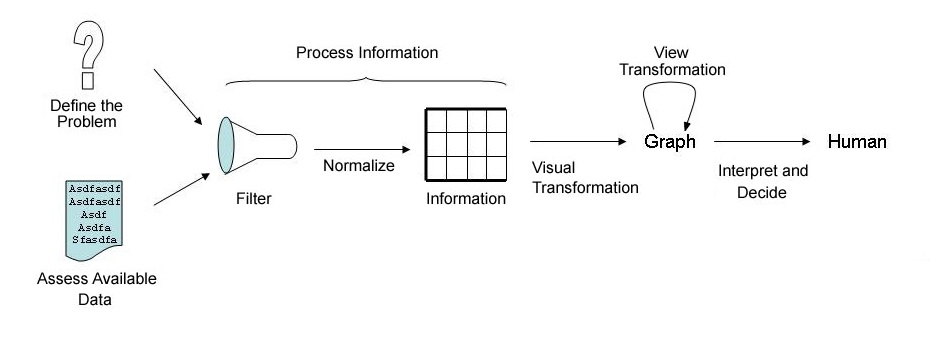
\includegraphics[width=1\textwidth]{visualization_process}
\caption{The Visualization Process}
\label{fig:visprocess}
\end{figure}

This process, as shown in Figure~\ref{fig:visprocess}, involves the creation phase as well as the interpretation of the resulting image by humans in order to gain a mental model and make sense of the data shown. The viewing of a graphical encoding of data should cause an ``Ah-ha!'' reaction in the viewer in the sense that a useful discovery has been made. Information designers can only control the visualization stage with the goal that interpretation of the result is as easy as possible~\cite{Holmberg06}. More specifically, the creation of visualizations involves the application of methods to map data to suitable structures, which can then be encoded through visual properties (like height, size, color etc.).

% We'll examine the respective applicability of interaction for the technologies we investigate.

\section{Computational Support}
%%%-----------------------------------------------------------------------------

According to Spence~\cite{InformationVisualization07}, computers have been responsible for massive advances in the field of Information Visualization.

There are three principal reasons why computational support has huge importance. First, because of \emph{inexpensive and fast memory access}, the storage of truly \emph{vast amounts of data} has become affordable for businesses and governments. Second, with powerful and fast computation mechanisms, the processing of data in realtime enables a number of tasks that are helpful for visually investigating data. Data can be \emph{filtered}, \emph{aggregated} and \emph{transformed} interactively for flexible exploration. This interactivity forms a great advantage of computer-aided visualizations when compared to their equivalents in print, which are static. Users may start exploring information by looking at the whole dataset through an aggregated synoptic view and request details on demand. Third, Spence states that the availability of high resolution graphic displays ensures that the presentation of data matches the power of human visual and cognitive systems. 

Computer graphics is not a new subject, neither is Interactive Information Visualization. Many software products have been developed and released in the last 20-30 years. Among these are graphically intensive \emph{Computer Games}, and \emph{Visual Analysis Tools} targeting all imaginable domains of life. However, in this thesis only technologies that are natively supported by current web browsers are examined, while taking into account the special characteristics of this environment when utilized as a medium. Visualization designers are dealing with a client-server scenario that offers a number of capabilities but also introduces limitations that must be considered.

While the choice of a graphical representation can impact the effectiveness of a visualization, this thesis first and foremost addresses the choice of technology as well as the utilization of suitable methods in terms of software design. A major requirement for all technology options is the support of arbitrary visual representations. Thus, this thesis will give a closer look on both \emph{low level graphical systems} and \emph{higher level visualization frameworks}. It will rather neglect ready-to-use charting libraries which are useful for quickly plotting common data structures but typically lack options for extensive customization. Another key aspect of web-based visualization is the support of interaction, since users can interact with their web-browser using mouse, keyboard or touch surfaces.


\section{The Human User}
%%%-----------------------------------------------------------------------------

With the availability of immense computational power to transform data and create visual output, designers sometimes lose sight of the user being the main consumer of visualizations. As Spence states, visualization is all about how human beings interact with data and how to graphically encode and present data best~\cite{InformationVisualization07}. It is important that the visualization designer is aware of the needs of a user as well as the characteristics of human behavior. This awareness cannot be emphasized enough. A lot of attempts end up in being beautiful, in terms of visually appealing for the eye, but make it hard for the user to make sense of it. Such visualizations are perfectly fine when created in the context of an artistic target, but fail when they are meant to transport information straight away.


\section{The Value of Information Visualization}
%%%-----------------------------------------------------------------------------

Without doubt, the topic of Information Visualization is fascinating, yet the question of its true value is important too~\cite{InformationVisualization07}. This value becomes obvious in many concrete application scenarios.


\subsection{Visual Analytics}
%%%-----------------------------------------------------------------------------

Visual Analytics developed out the fields of Information Visualization and Scientific Visualization and has a strong focus on analytical reasoning.

According to Ziemkiewicz and Kosara~\cite{Ziemkiewicz10}, it combines classical data analysis techniques with those of Information Visualization. In an analysis scenario with the help of Information Visualization users can explore a large amounts of data using visual tools in order to reveal patterns which are not obvious when looking at the raw data.

The importance of Visual Analytics was also recognized by the U.S. Department of Homeland Security when they chartered the National Visualization and Analytics Center (NVAC) in 2004. The goal was to help avoiding future terrorist attacks in the U.S. and around the globe. A lot of groundwork has been done by the NVAC, not least have they contributed a five year research and development agenda for Visual Analytics. \emph{Illuminating the Path - The Research and Development Agenda for Visual Analytics}~\cite{IlluminatingThePath05} addresses the most important needs in R\&D to gain advanced analytical insight. According to them, Visual Analytics is a multidisciplinary field that includes the following focus areas:

\begin{itemize}
\item Analytical reasoning techniques that enable users to obtain deep insights that directly support assessment, planning, and decision making.
\item Visual representations and interaction techniques that take advantage of the human eye's broad bandwidth pathway into the mind to allow users to \emph{see}, \emph{explore}, and \emph{understand} large amounts of information at once.
\item \emph{Data representations} and \emph{transformations} that convert all types of conflicting and dynamic data in ways that support visualization and analysis.
\item Techniques to support \emph{production}, \emph{presentation}, and \emph{dissemination} of the results of an analysis to communicate information in the appropriate context to a variety of audiences.
\end{itemize}

\SuperPar Even though Information Visualization is not limited to the field of Visual Analytics, it is without doubt a major field of application. Thus, techniques and approaches described in this thesis were not developed without bearing Visual Analytics as a main application scenario in mind.


\subsection{Exploratory Data Analysis}
%%%-----------------------------------------------------------------------------


Fluit et. al describe the task of data exploration as a process of information search, that is \emph{not of immediate relevance}~\cite{Fluit05}. The difference between data exploration and querying is that \emph{no particular questions are to be answered}. Instead, users get an \emph{overview} of the complete information available and start to make sense of it by digging deeper into the data and viewing certain aspects, but without losing the overall context. The goal here is that users become familiar with the dataset and figure out how it is structured and organized. Based on knowledge gained through exploration, users are able to formulate specific questions afterwards. In order to make possible Exploratory Data Analysis, \emph{Filtering}, \emph{Zooming} and \emph{Detail-on-demand} functionality must be supported by the visualization.

\subsection{Collaborative Visualization}
%%%-----------------------------------------------------------------------------

\begin{figure}
\centering
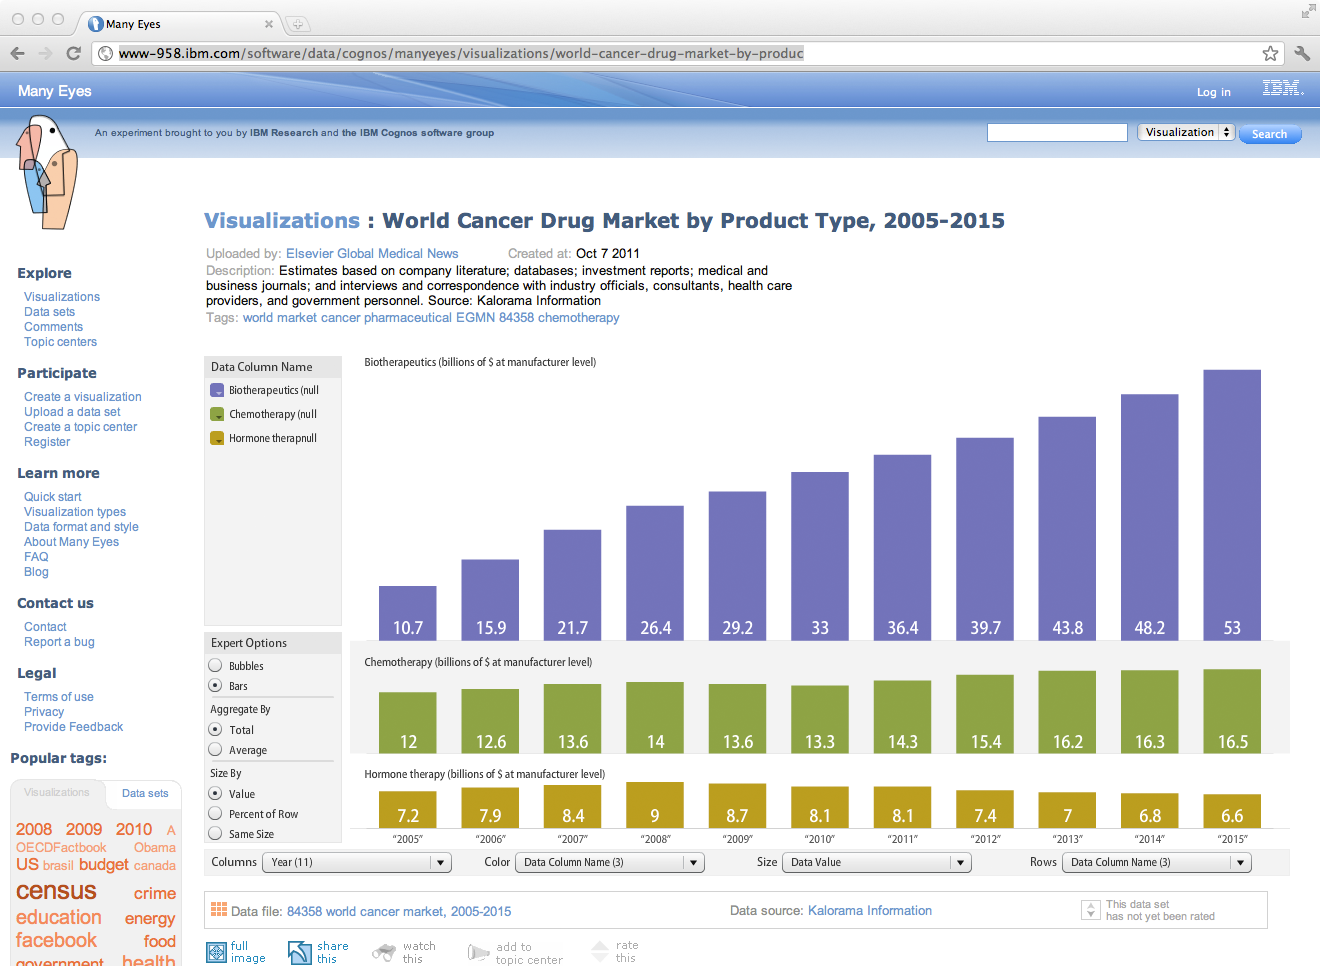
\includegraphics[width=1\textwidth]{manyeyes}
\caption{ManyEyes: Showing a visualization of the World Cancer Drug Market }
\label{fig:manyeyes}
\end{figure}

According to Heer et. al, visualizations are not just analytic tools but social spaces~\cite{voyagers-and-voyeurs,design-considerations-vast}. Visual systems improve our ability to process large amounts of data and enable visual sense-making. Sense-making is a social process, as people interpret data differently~\cite{card99}. This triggers a collective discourse and eventually either leads to consensus or people learn from their peers. Moreover, some datasets are too large to be examined by one person. Using a collaborative interface, a task can be divided into sub-tasks.

Discussions about trends are often scattered and disconnected from the actual visualization~\cite{voyagers-and-voyeurs}. Communication still takes place through email or other classic channels. Resulting from this it is getting difficult for newcomers to catch up and even the review process becomes harder. Thus, discussions should take place right at the visualization workspace.

\begin{figure}
\centering
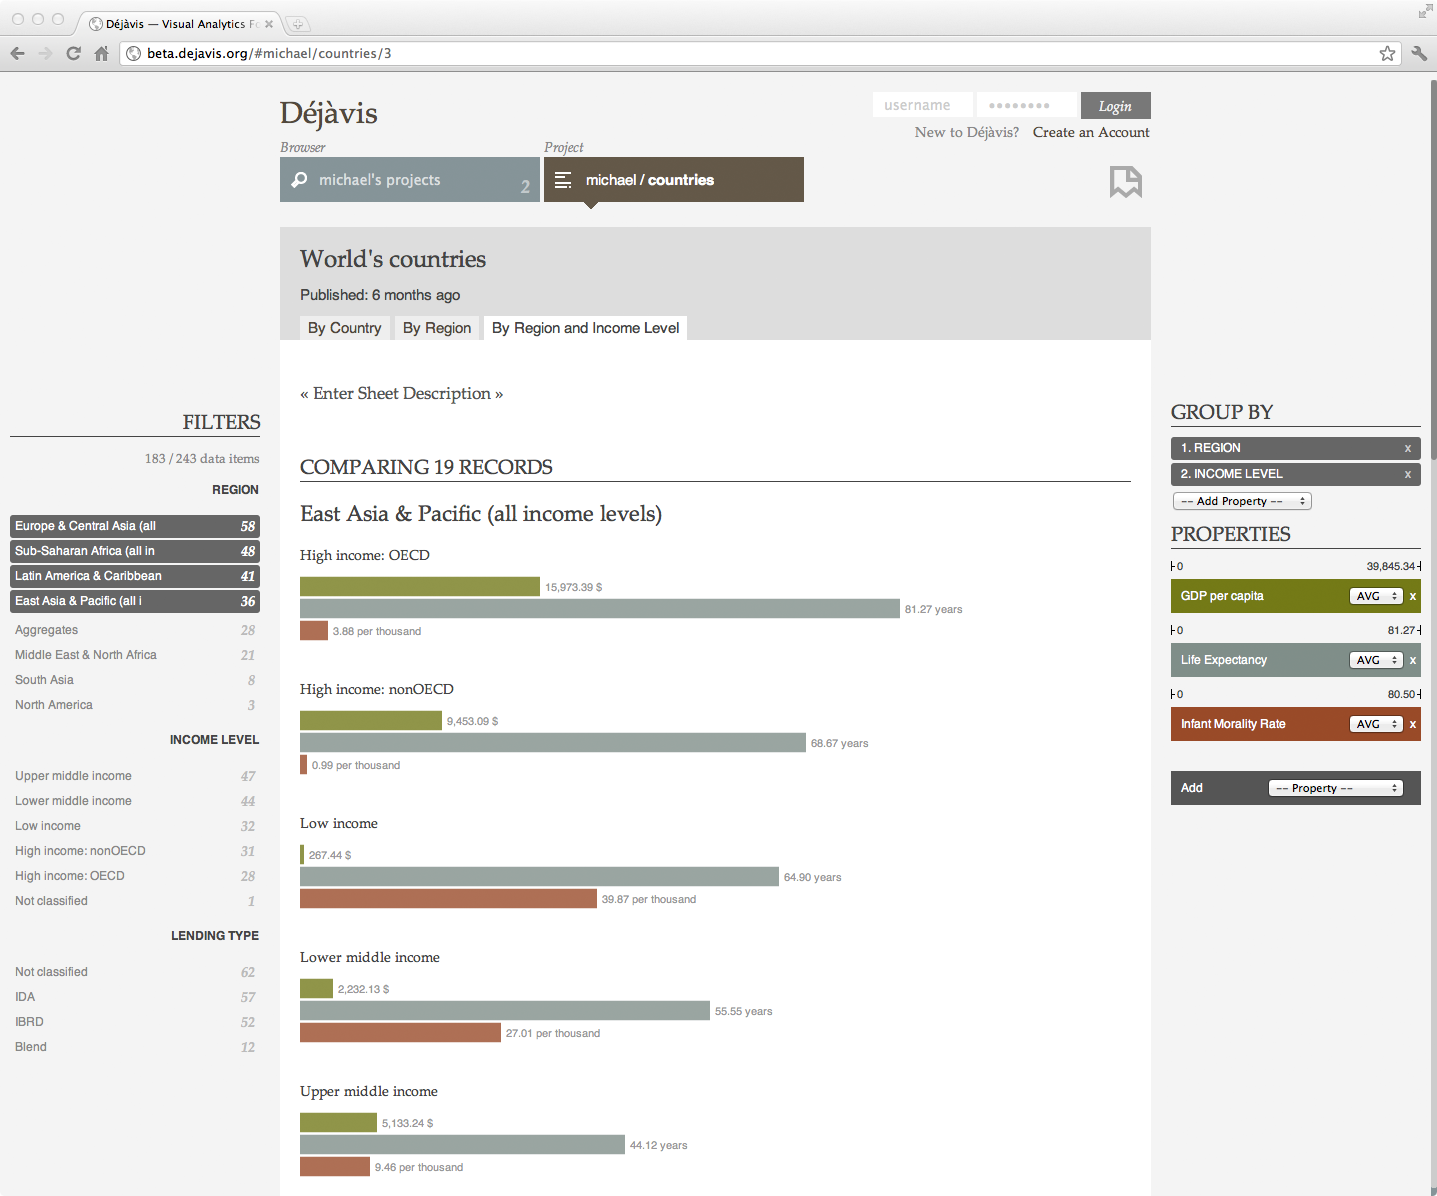
\includegraphics[width=1\textwidth]{dejavis}
\caption{Dejavis: Showing an analysis of the world's countries by various numerical indicators (such as GDP per capita, life expectancy, infant mortality rate).}
\label{fig:dejavis}
\end{figure}

In order to ease the task of exchanging insight discovered on a particular dataset, application bookmarks are important. If the current application state (user settings, data-source) could be stored and made available using a public URL, knowledge can be shared easily with others. This is referred to as \emph{View Sharing} in literature~\cite{clark91}.

A prominent example for such a social data analysis tool is ManyEyes\footnote{http://many-eyes.com}, shown in Figure~\ref{fig:manyeyes}, an IBM research experiment~\cite{manyeyes}. Dejavis\footnote{http://beta.dejavis.org}, as shown in Figure~\ref{fig:dejavis}, is another example, contributed by the author. It supports \emph{View Sharing} \cite{clark91} and \emph{Contextual Data Transformations} \cite{manyeyes}.


\begin{figure}
\centering
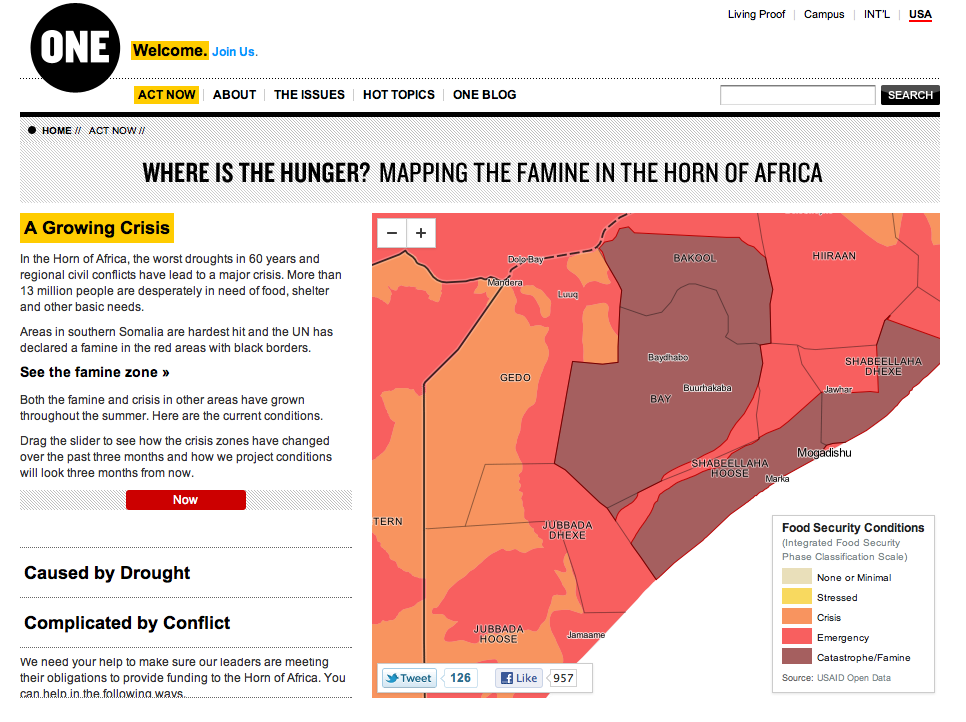
\includegraphics[width=1\textwidth]{horn}
\caption{Where is the Hunger: Mapping the famine in the Horn of Africa.}
\label{fig:horn}
\end{figure}

\subsection{Narrative Visualization}
%%%-----------------------------------------------------------------------------


One promising new field is called Narrative Visualization, which can be described as \emph{telling stories with data}.  Information Visualization, with its ability to reveal narratives within data, is a great way to communicate stories in new different ways~\cite{NarrativeVis10}. Story tellers, like online journalists increasingly start adapting visualizations into their online stories. In some cases the visualization entirely functions in place of a written story. Where is the hunger\footnote{http://one.org/us/actnow/horn.html} (see Figure~\ref{fig:horn}), visually tells the story of the famine in the Horn of Africa.


\section{The Information Seeking Mantra}
%%%-----------------------------------------------------------------------------

According to Shneiderman~\cite{shneiderman96eyes} the bandwidth of information presentation is potentially higher in the visual domain than in any other media. After having completed many projects, he has identified the following principle that applies to the majority of visualization scenarios:

\begin{quotation}
    ``Overview first, zoom and filter, then details-on-demand''
\end{quotation}

\SuperPar This principle is referred to as \emph{The Information Seeking Mantra} and serves as a starting point for creating visualizations. Based on that, Shneiderman also proposes a Task by Data Type Taxonomy (TTT) with seven data types (1-, 2-, 3-dimensional data, temporal data, multi-dimensional data, and tree and network data) and seven tasks (overview, zoom, filter, details-on-demand, relate, history, and extract). In response to Shneiderman the following sections will introduce these \emph{Tasks} and \emph{Data Types} using illustrative examples.

\section{The Tasks} % originally the Issues
\label{sec:tasks}
%%%-----------------------------------------------------------------------------


Based on a particular problem scope, namely the examination of a set of documents, Shneiderman's \emph{Tasks}~\cite{shneiderman96eyes} are identified and described. Documents under investigation are associated with a set of terms mentioned in these documents. The goal is to find relevant documents according to one or more selected terms. Instead of using a full text search (fuzzy information retrieval), a method called \emph{Faceted Navigation}~\cite{Huynh09} is used to explore the set of available documents interactively. Since the documents are annotated with categorized entities that belong to those documents, users can easily ask for the values of a specific entity type (like authors). Only values (entities) that are mentioned within the set of documents are displayed. In other words, there is always at least one document match per entity.


% \subsection{The data}
%%%-----------------------------------------------------------------------------

Our example dataset shows a number of documents that are related to Information Visualization Libraries. Each document is annotated with attributes which are specific for this particular one.

\begin{center}
    \begin{tabular}{ | l | l | l | p{2.3cm} |}
    \hline
    Title & Authors & Technolgies used \\ \hline
    Protovis & Michael Bostock, Jeffery Heer & SVG, Javascript  \\ \hline
    D3.js & Michael Bostock & SVG, Javascript, CSS \\ \hline
    Processing.js & John Resig & Canvas, Javascript \\ \hline
    Unveil.js & Michael Aufreiter & Canvas, Javascript, JSON \\ \hline
    Raphael & Dmitry Baranovskiy & SVG, Javascript \\ \hline
    Paper.js & J\"urg Lehni, Jonathan Puckey & Canvas, Javascript \\ \hline
    \end{tabular}
\end{center}

\SuperPar \textbf{Table Presentation}

\SuperPar Although most people are familiar with tables, they often are of limited help, especially when they contain many rows and columns. It is hard for the viewer to find rows that match a particular set of criteria. The viewer has to step through the entire table, row by row, checking if the wanted criteria is met. At least some facility to rearrange table rows according to some criterion would be helpful \cite{InformationVisualization07}.

\SuperPar \textbf{Graphical Abstraction}

\SuperPar Since the table representation is hard to read, a suitable graphical abstraction is needed in order to encode documents visually. Figure \ref{fig:overview} shows the same set of documents, but this time arranged on a matrix-grid.


\subsection{Overview}
%%%-----------------------------------------------------------------------------

As Spence states, the term \emph{overview} cannot be defined easily with precision~\cite{InformationVisualization07}. However, the goal of an overview is to serve as an entry point, preparing the way for further examinations based on a dataset of interest. The user should be able to answer questions like: How many items are in the collection? Adequate overview strategies plus detail (also called context plus focus) are an important criteria to look for~\cite{shneiderman96eyes}.

The visualization, as shown in Figure~\ref{fig:overview}, not only displays available documents in a collection, but also a list of entities that are mentioned within those.

\begin{figure}
\centering
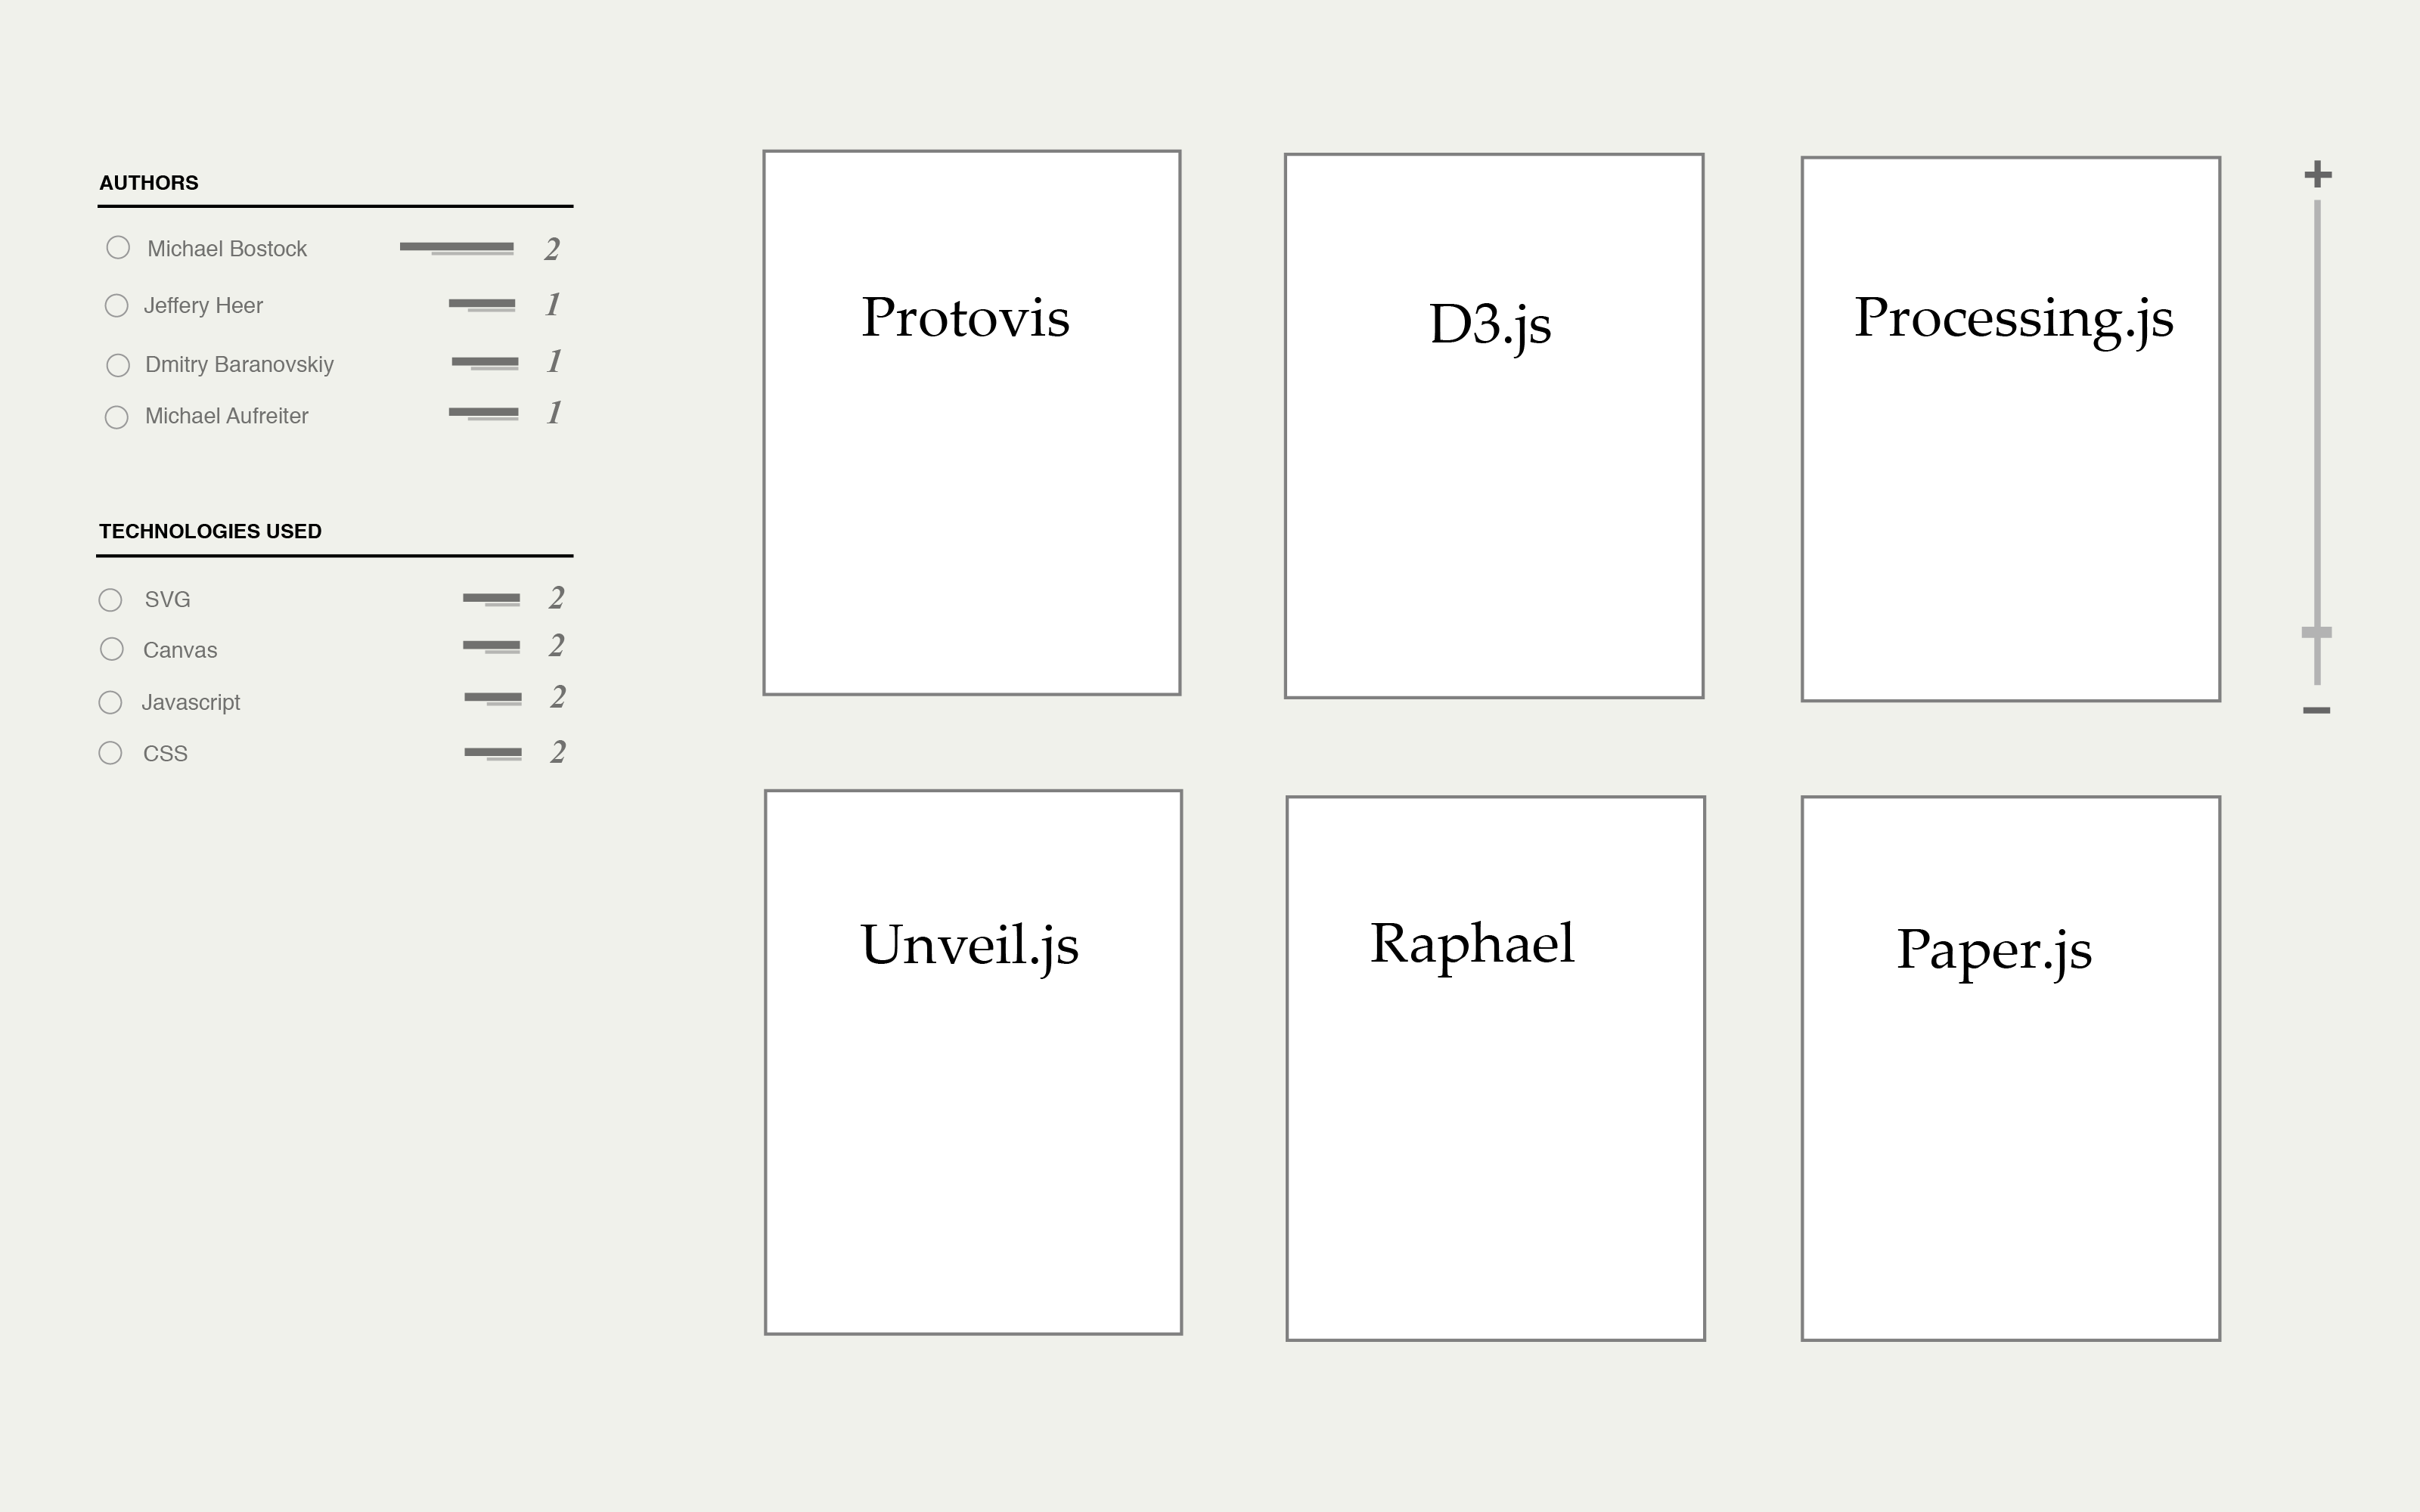
\includegraphics[width=1\textwidth]{doc_explorer/master_thesis_illustrations_2-01}
\caption{Overview: Shows all documents, along with a list of associated entities}
\label{fig:overview}
\end{figure}


\subsection{Zoom}
%%%-----------------------------------------------------------------------------

\begin{figure}
\centering
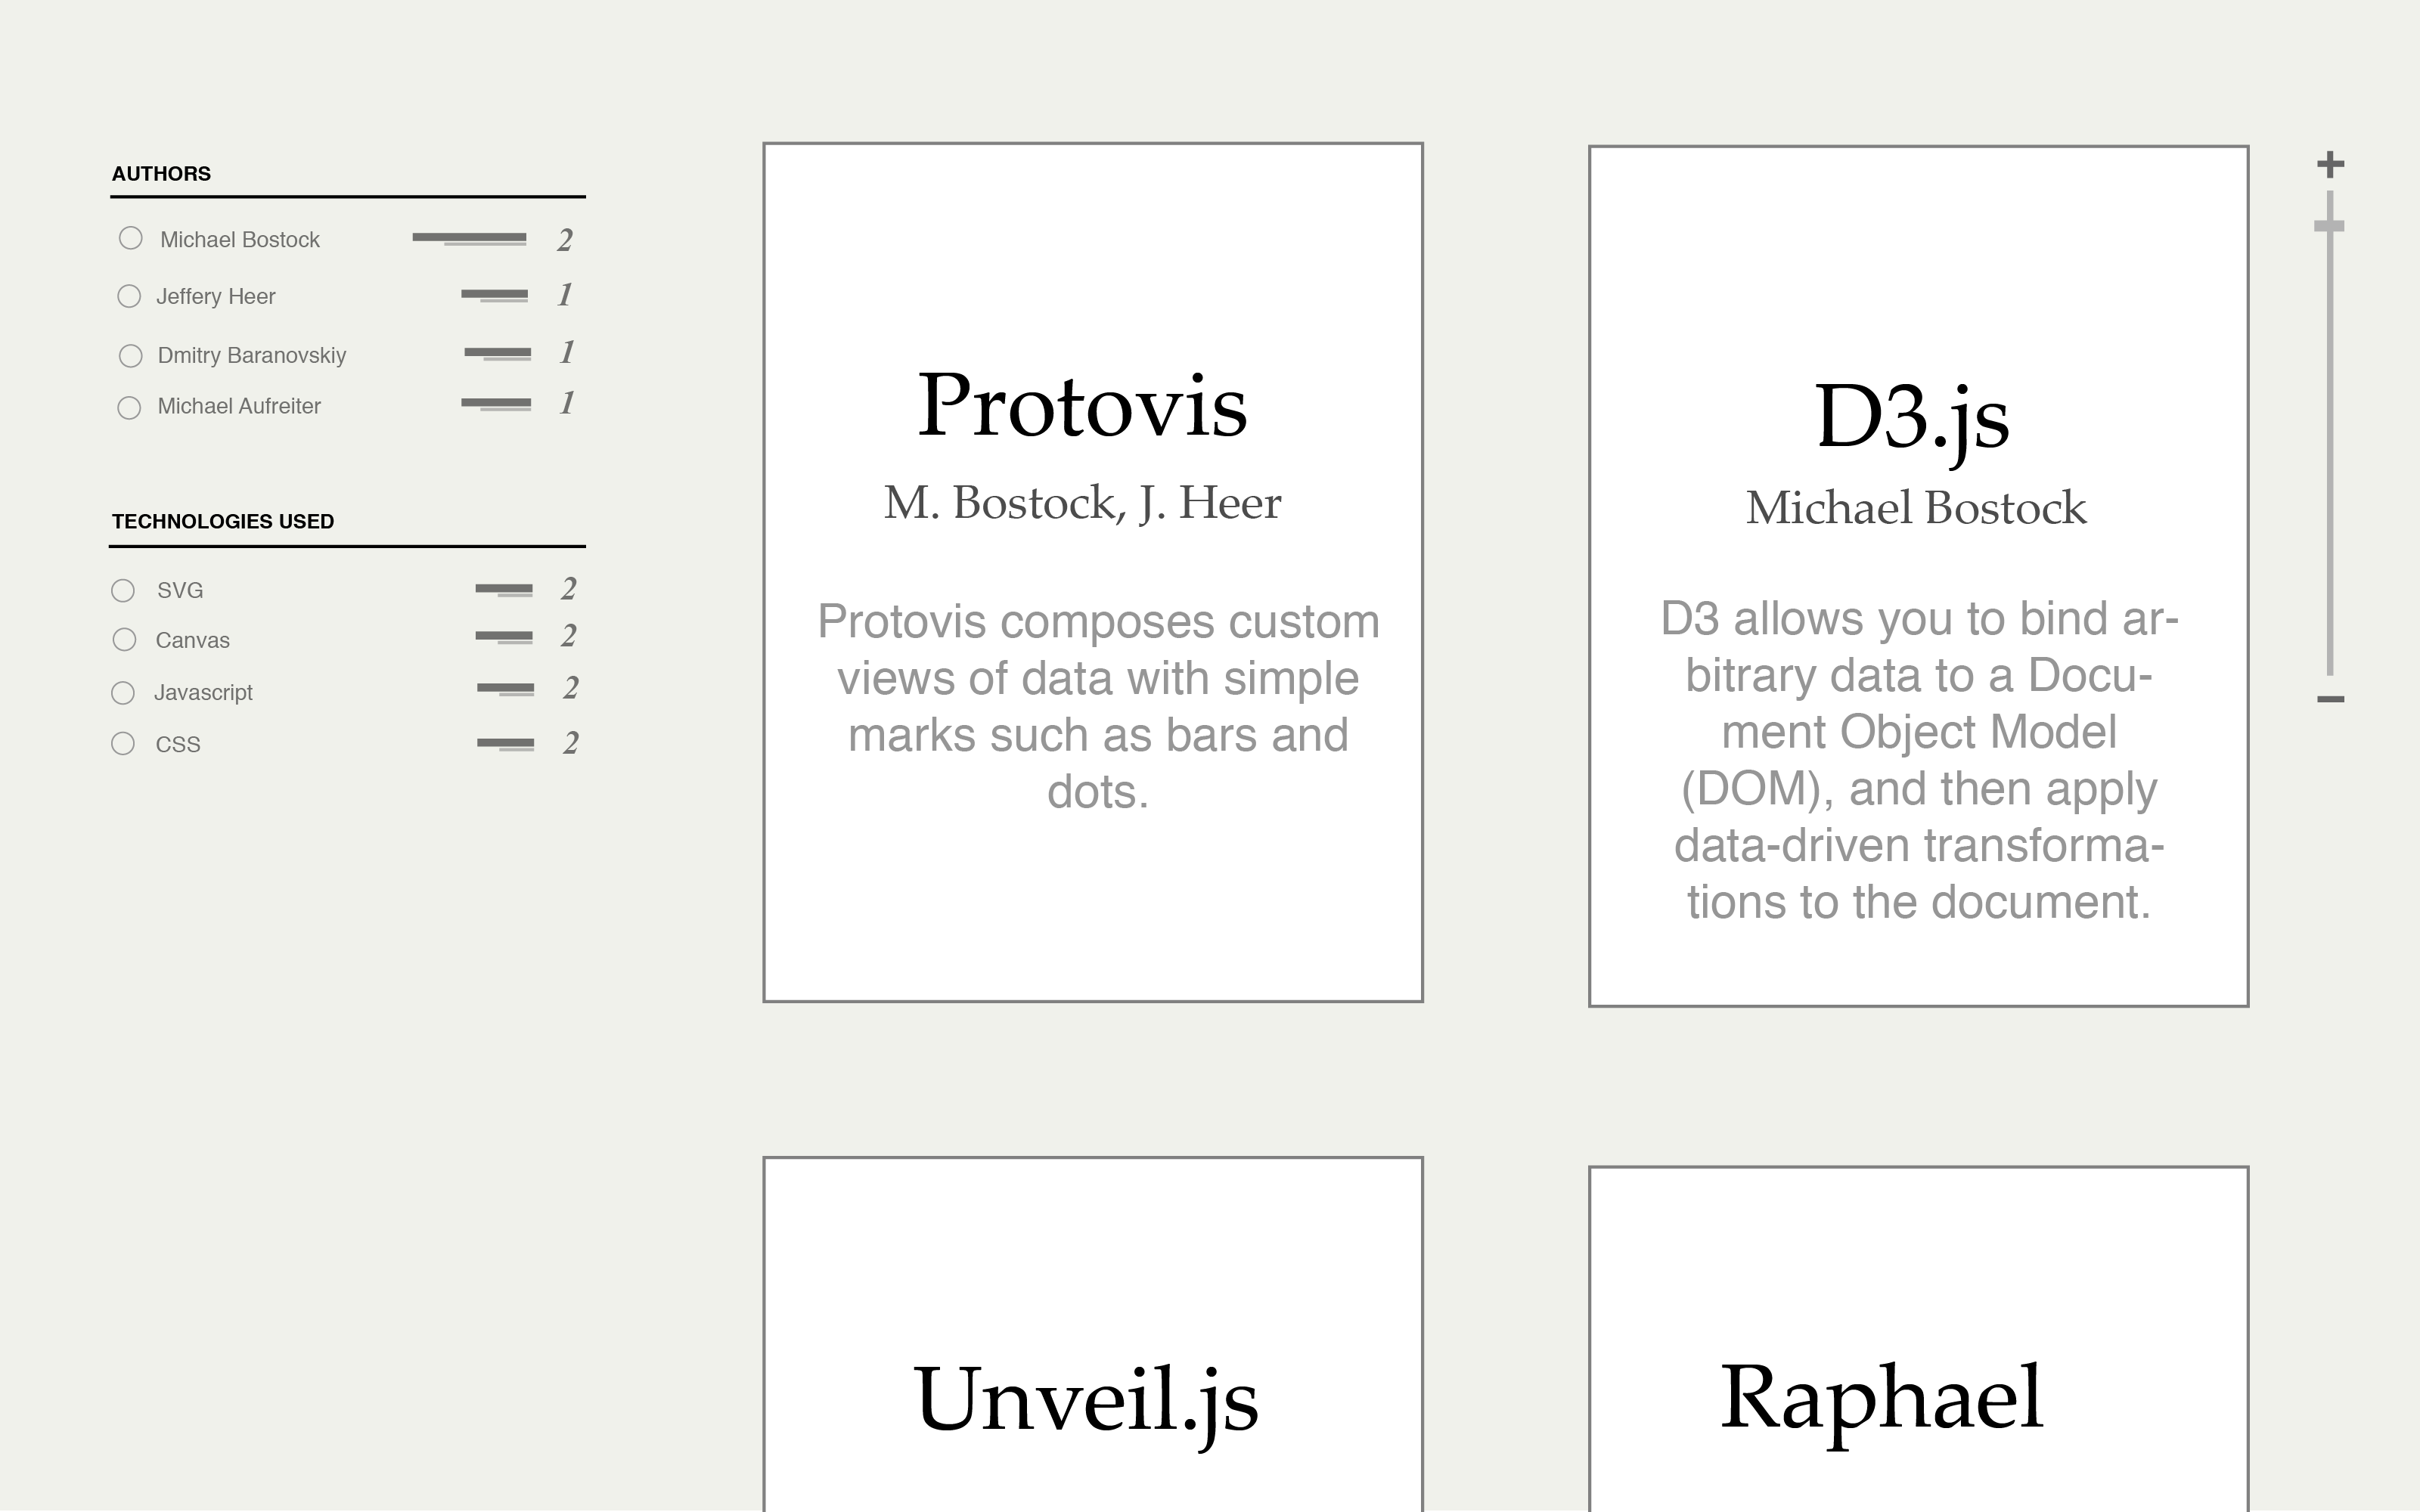
\includegraphics[width=1\textwidth]{doc_explorer/master_thesis_illustrations_2-02}
\caption{Zoom: Focus on the upper left area of the matrix plot}
\label{fig:zoom}
\end{figure}

A user might want to zoom in on items of interest. The user is likely to be interested in some portion of a collection. In order to focus on a particular area, control over the \emph{zoom focus} and \emph{zoom level} is needed. In Figure~\ref{fig:zoom} a user has zoomed into the upper left area. The increased zoom level unveils more details about the documents in focus, such as the author and a short abstract.

\subsection{Filter}
%%%-----------------------------------------------------------------------------

\begin{figure}
\centering
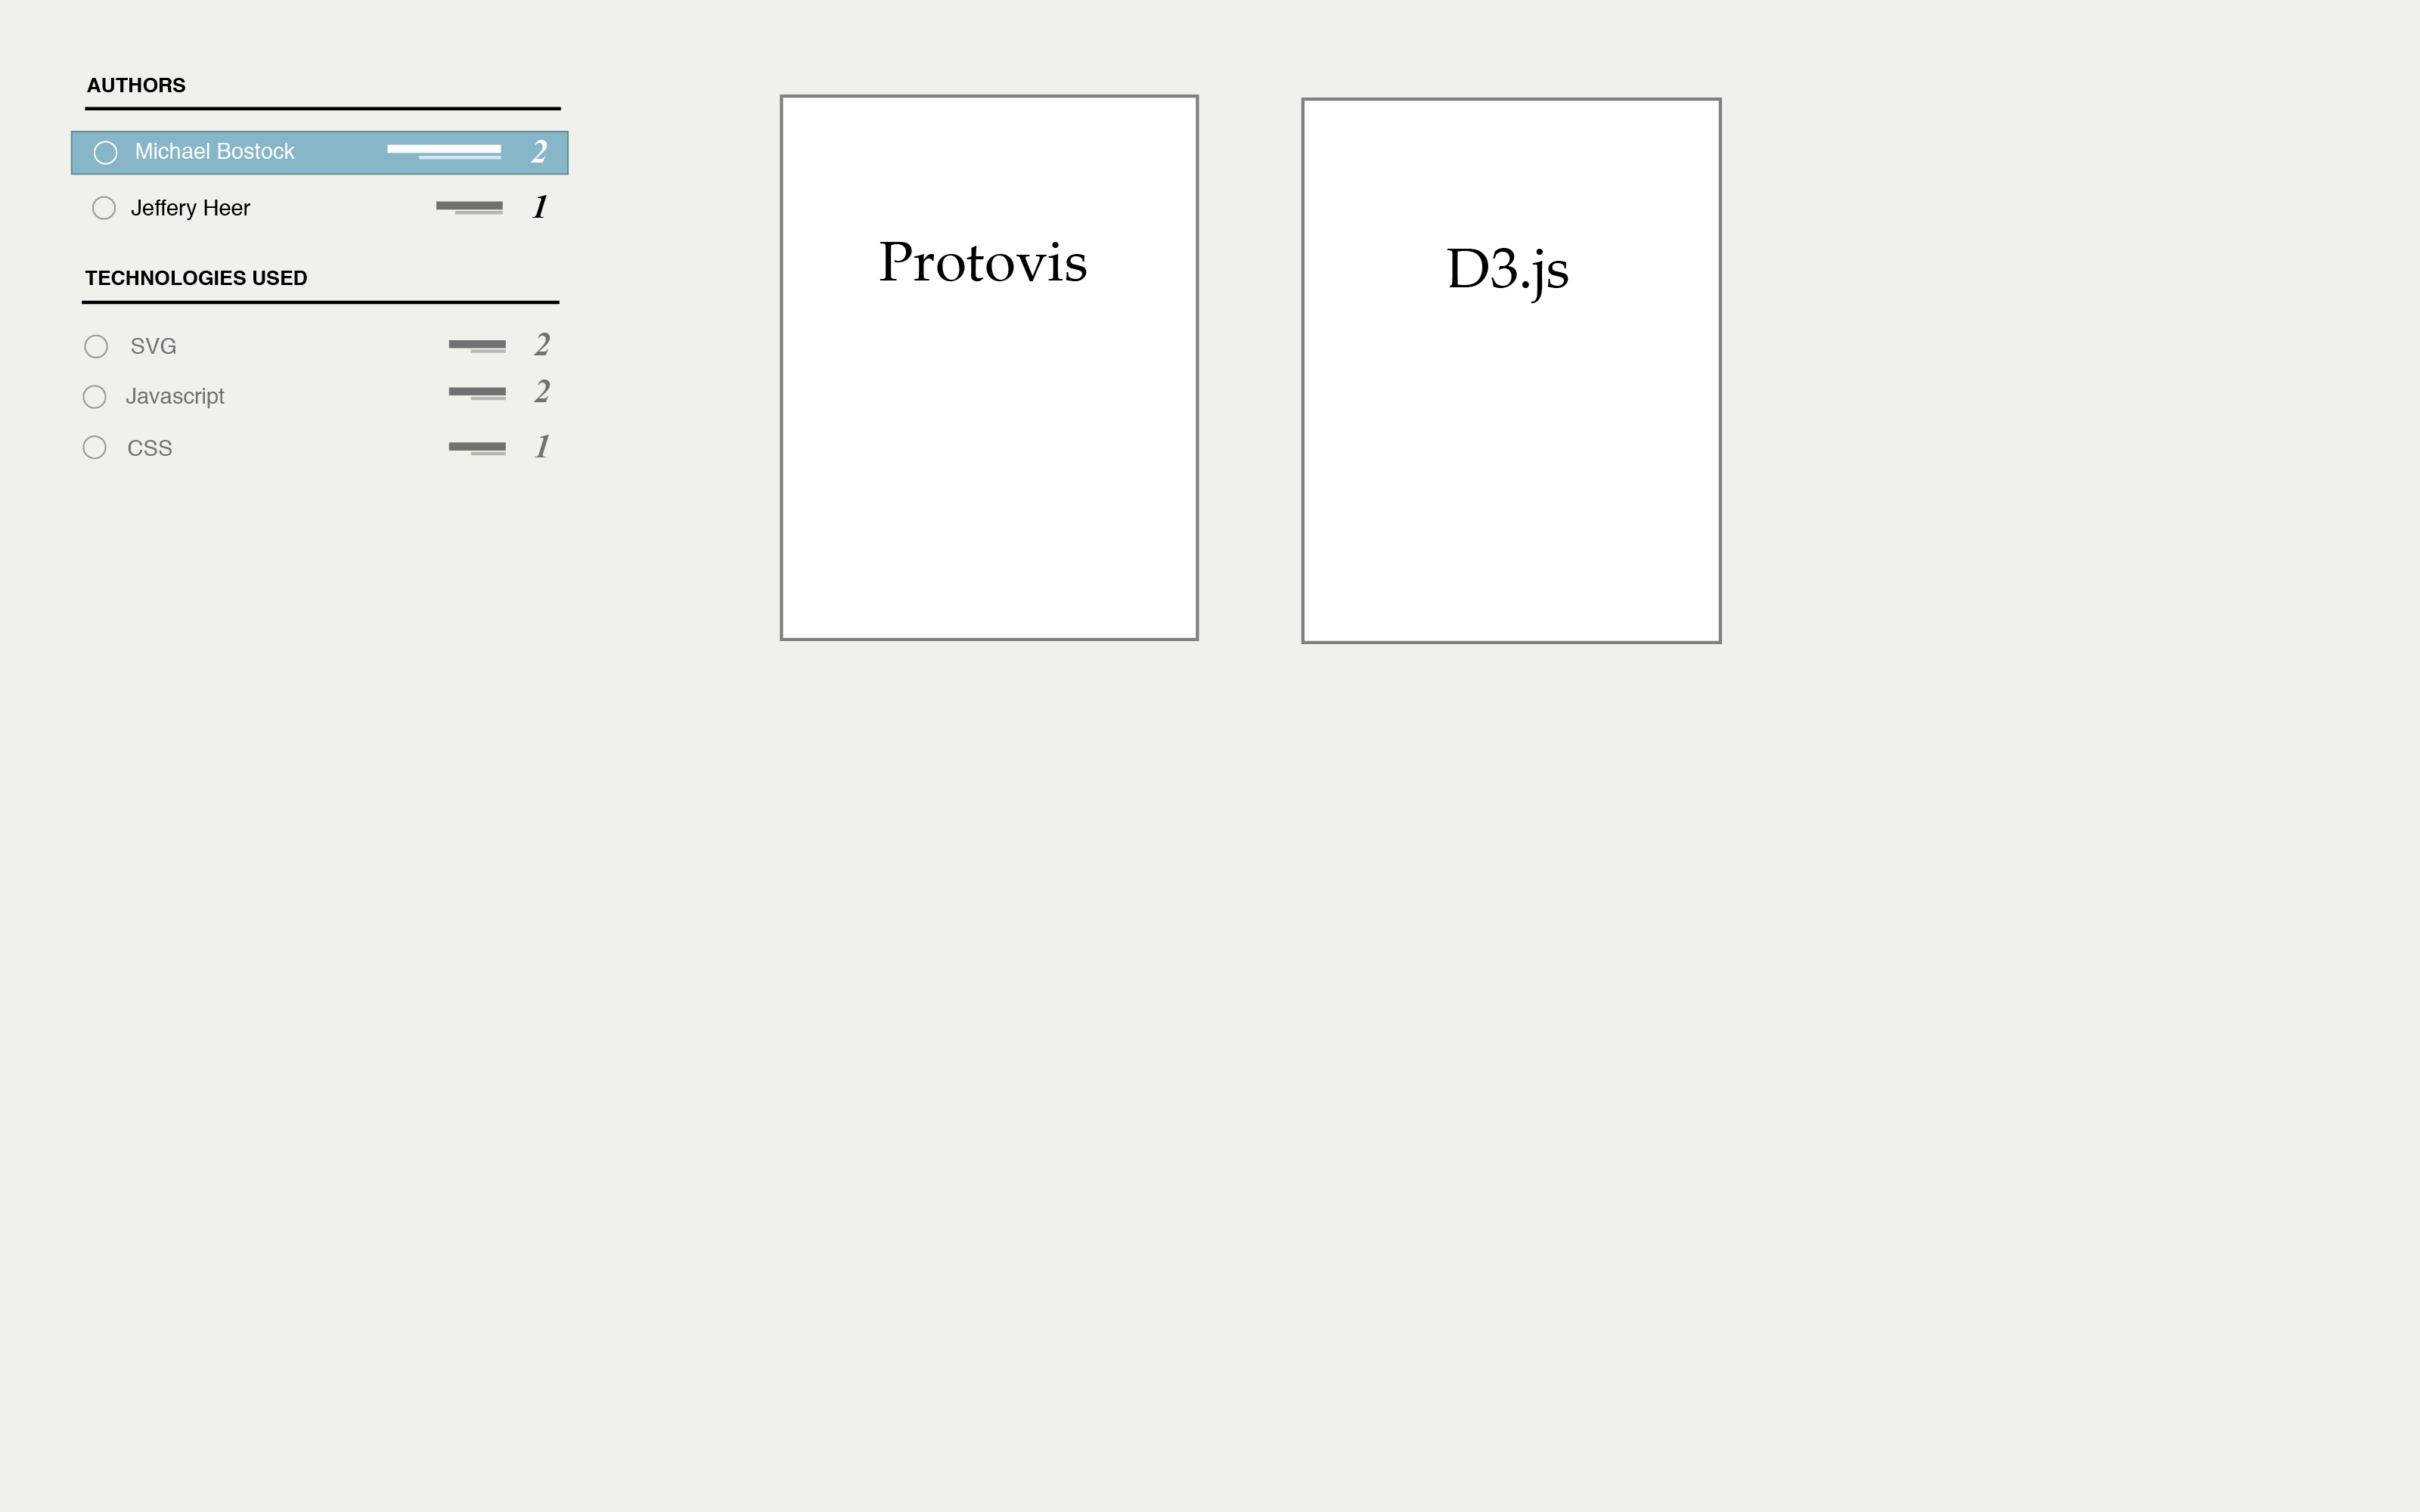
\includegraphics[width=1\textwidth]{doc_explorer/master_thesis_illustrations_2-05}
\caption{Filter: Filtering restricts the number of documents based on selected attributes}
\label{fig:filtering}
\end{figure}

Filtering allows the reduction of a dataset based on a user-defined set of criteria~\cite{Ahlberg92dynamicqueries}. Objects that do not match will no longer be included in the result. Filtering is an important tool for data exploration. It enables analysts to reveal facts that are not obvious when looking at the full dataset. Also implicit coherences can be discovered more easily. Thus, the quality of an interactive visualization depends to a high degree on the availability of extensive filtering options. Figure \ref{fig:filtering} shows a reduced set of documents based on a particular selection of entities.


\subsection{Details-on-demand}
%%%-----------------------------------------------------------------------------

\begin{figure}
\centering
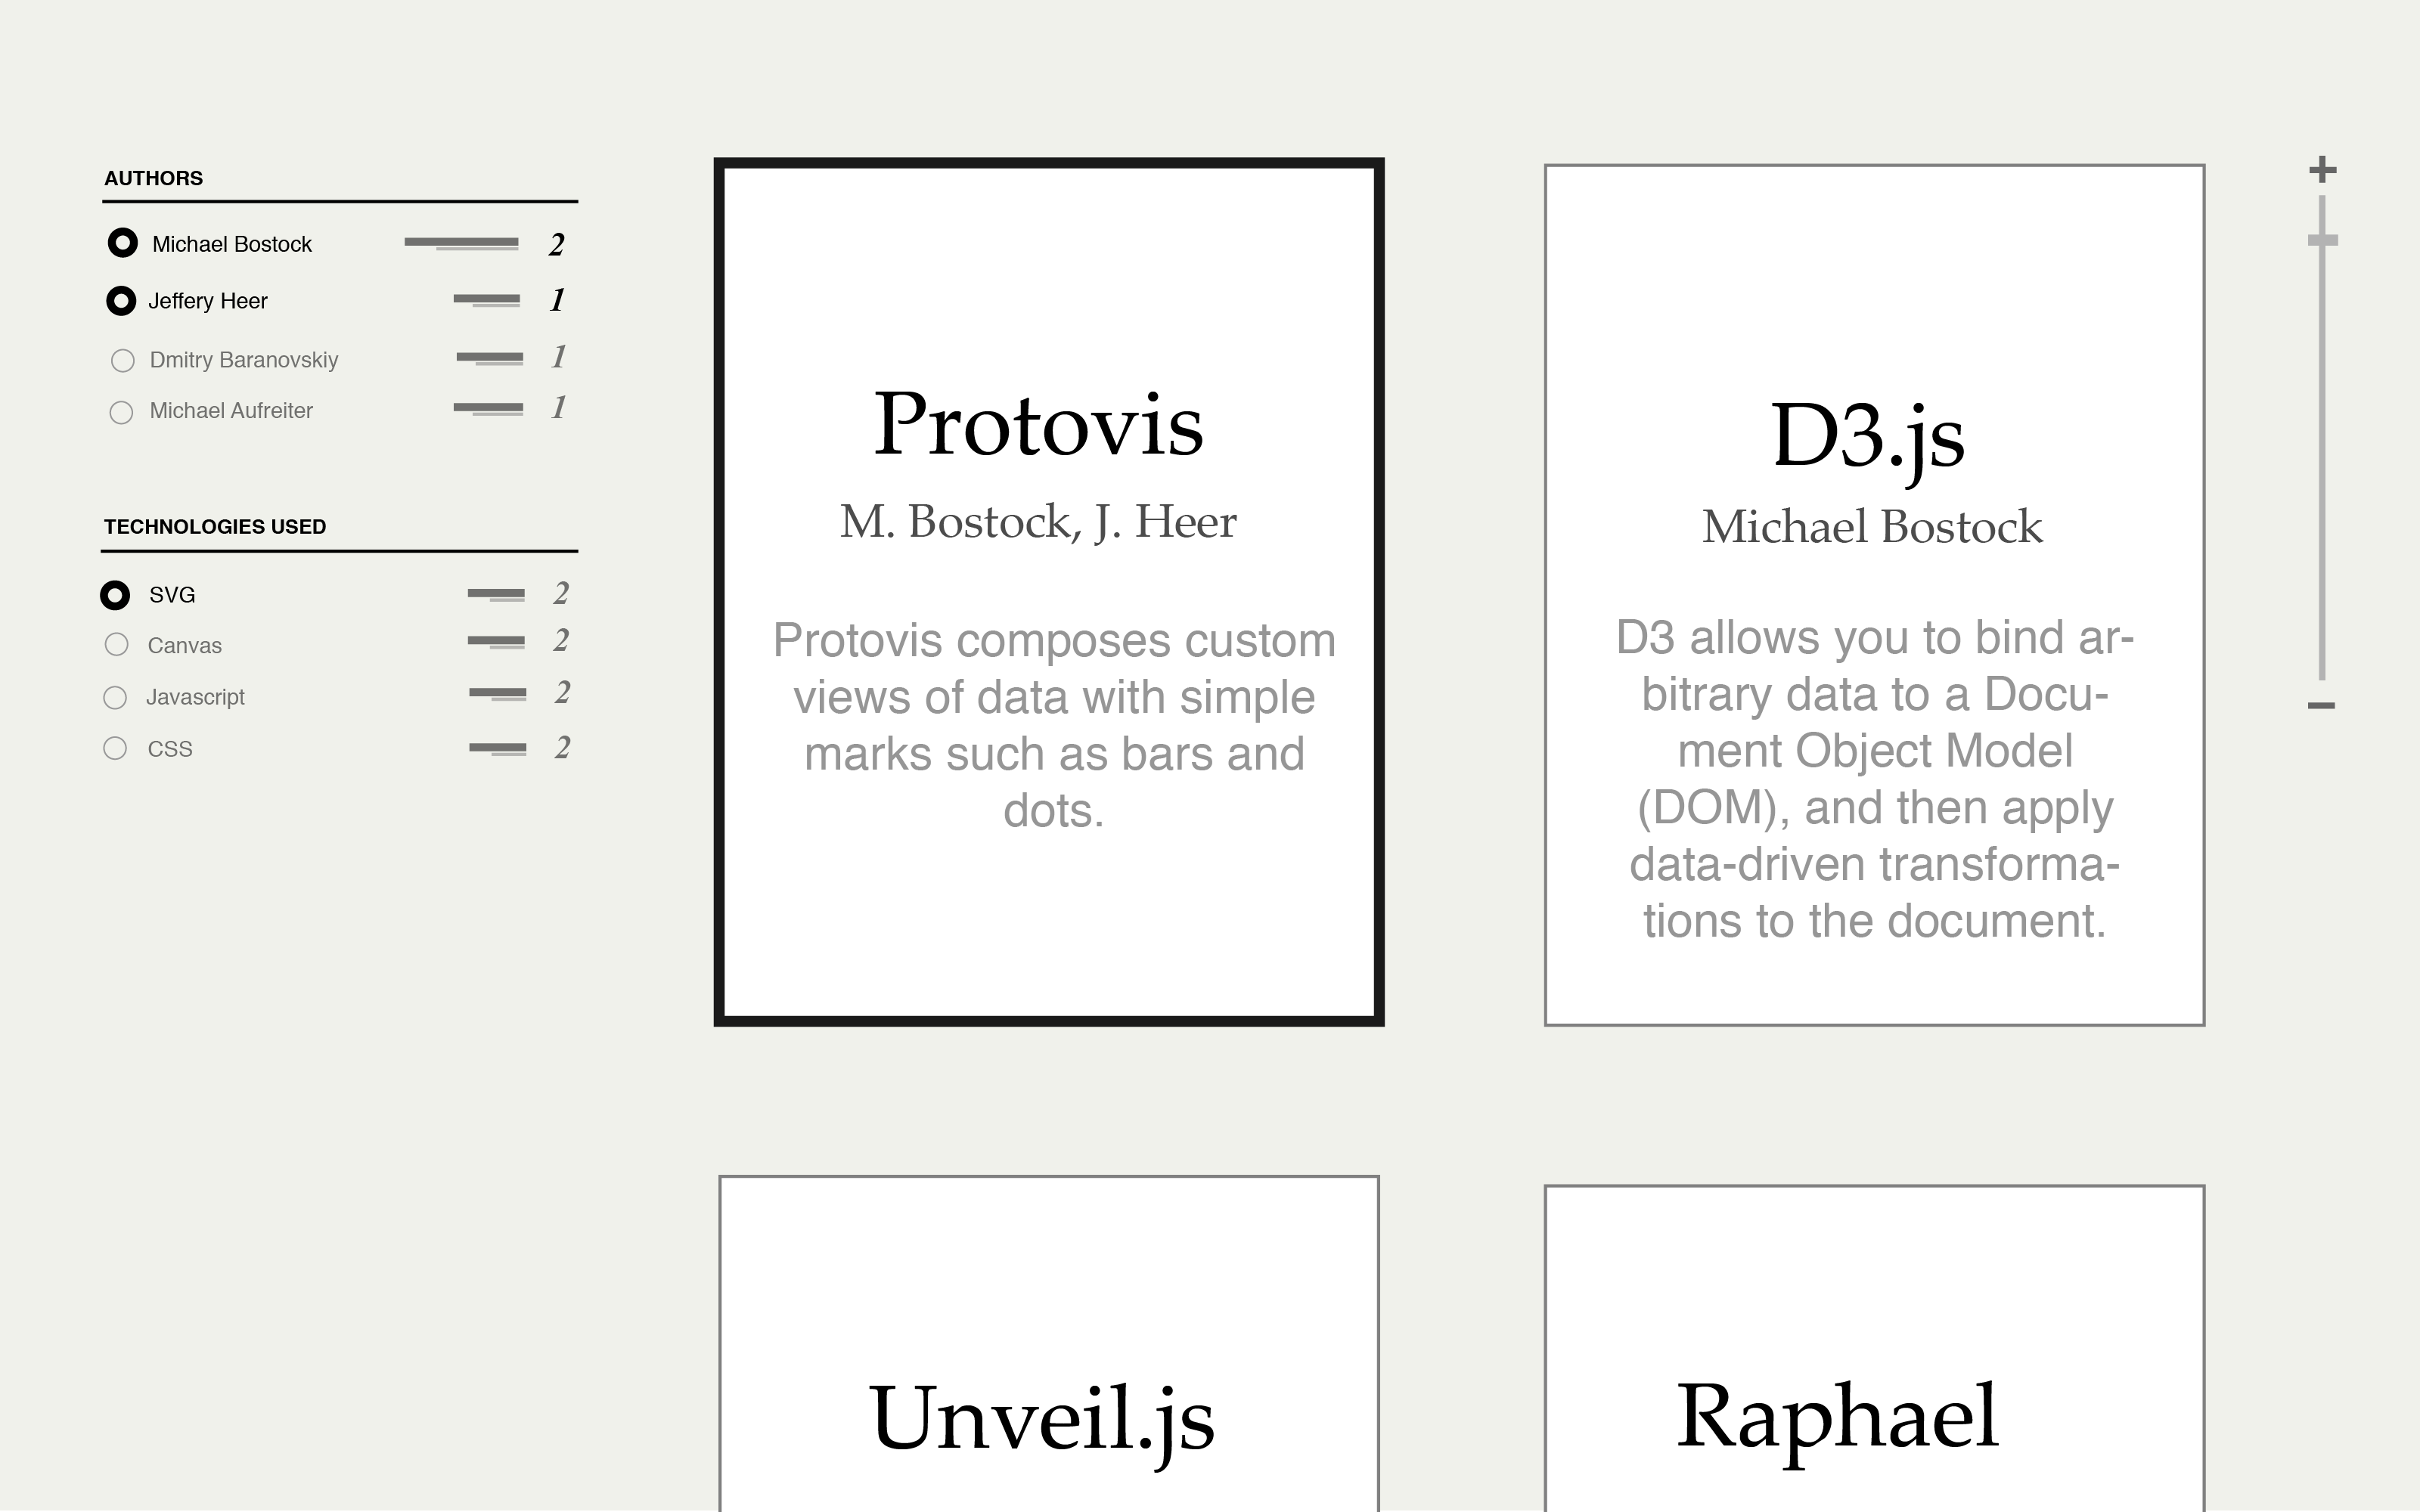
\includegraphics[width=1\textwidth]{doc_explorer/master_thesis_illustrations_2-03}
\caption{Detail-on-demand: For a certain object additional details, like associated entities are displayed}
\label{fig:detail}
\end{figure}

Users usually want to find out details for a selected object. This is usually done by providing a popup window containing the values of each attribute~\cite{shneiderman96eyes}. However, there are other options such as displaying contextual information based on the currently selected item, as shown in Figure~\ref{fig:detail}.


\subsection{Relate}
%%%-----------------------------------------------------------------------------

Viewing relationships between data items is also an important task. Based on an attribute selection, as shown in Figure \ref{fig:relate}, users can find out which documents are associated with both ``Michael Bostock'' and ``Jeffery Heer''. Color coding is used to connect documents with concrete attributes. In addition to that, size is used to encode relevance. Documents that contain all selected entities are displayed at maximum size while others, which only match one entity, appear smaller. Documents that do not match are greyed out.

\begin{figure}
\centering
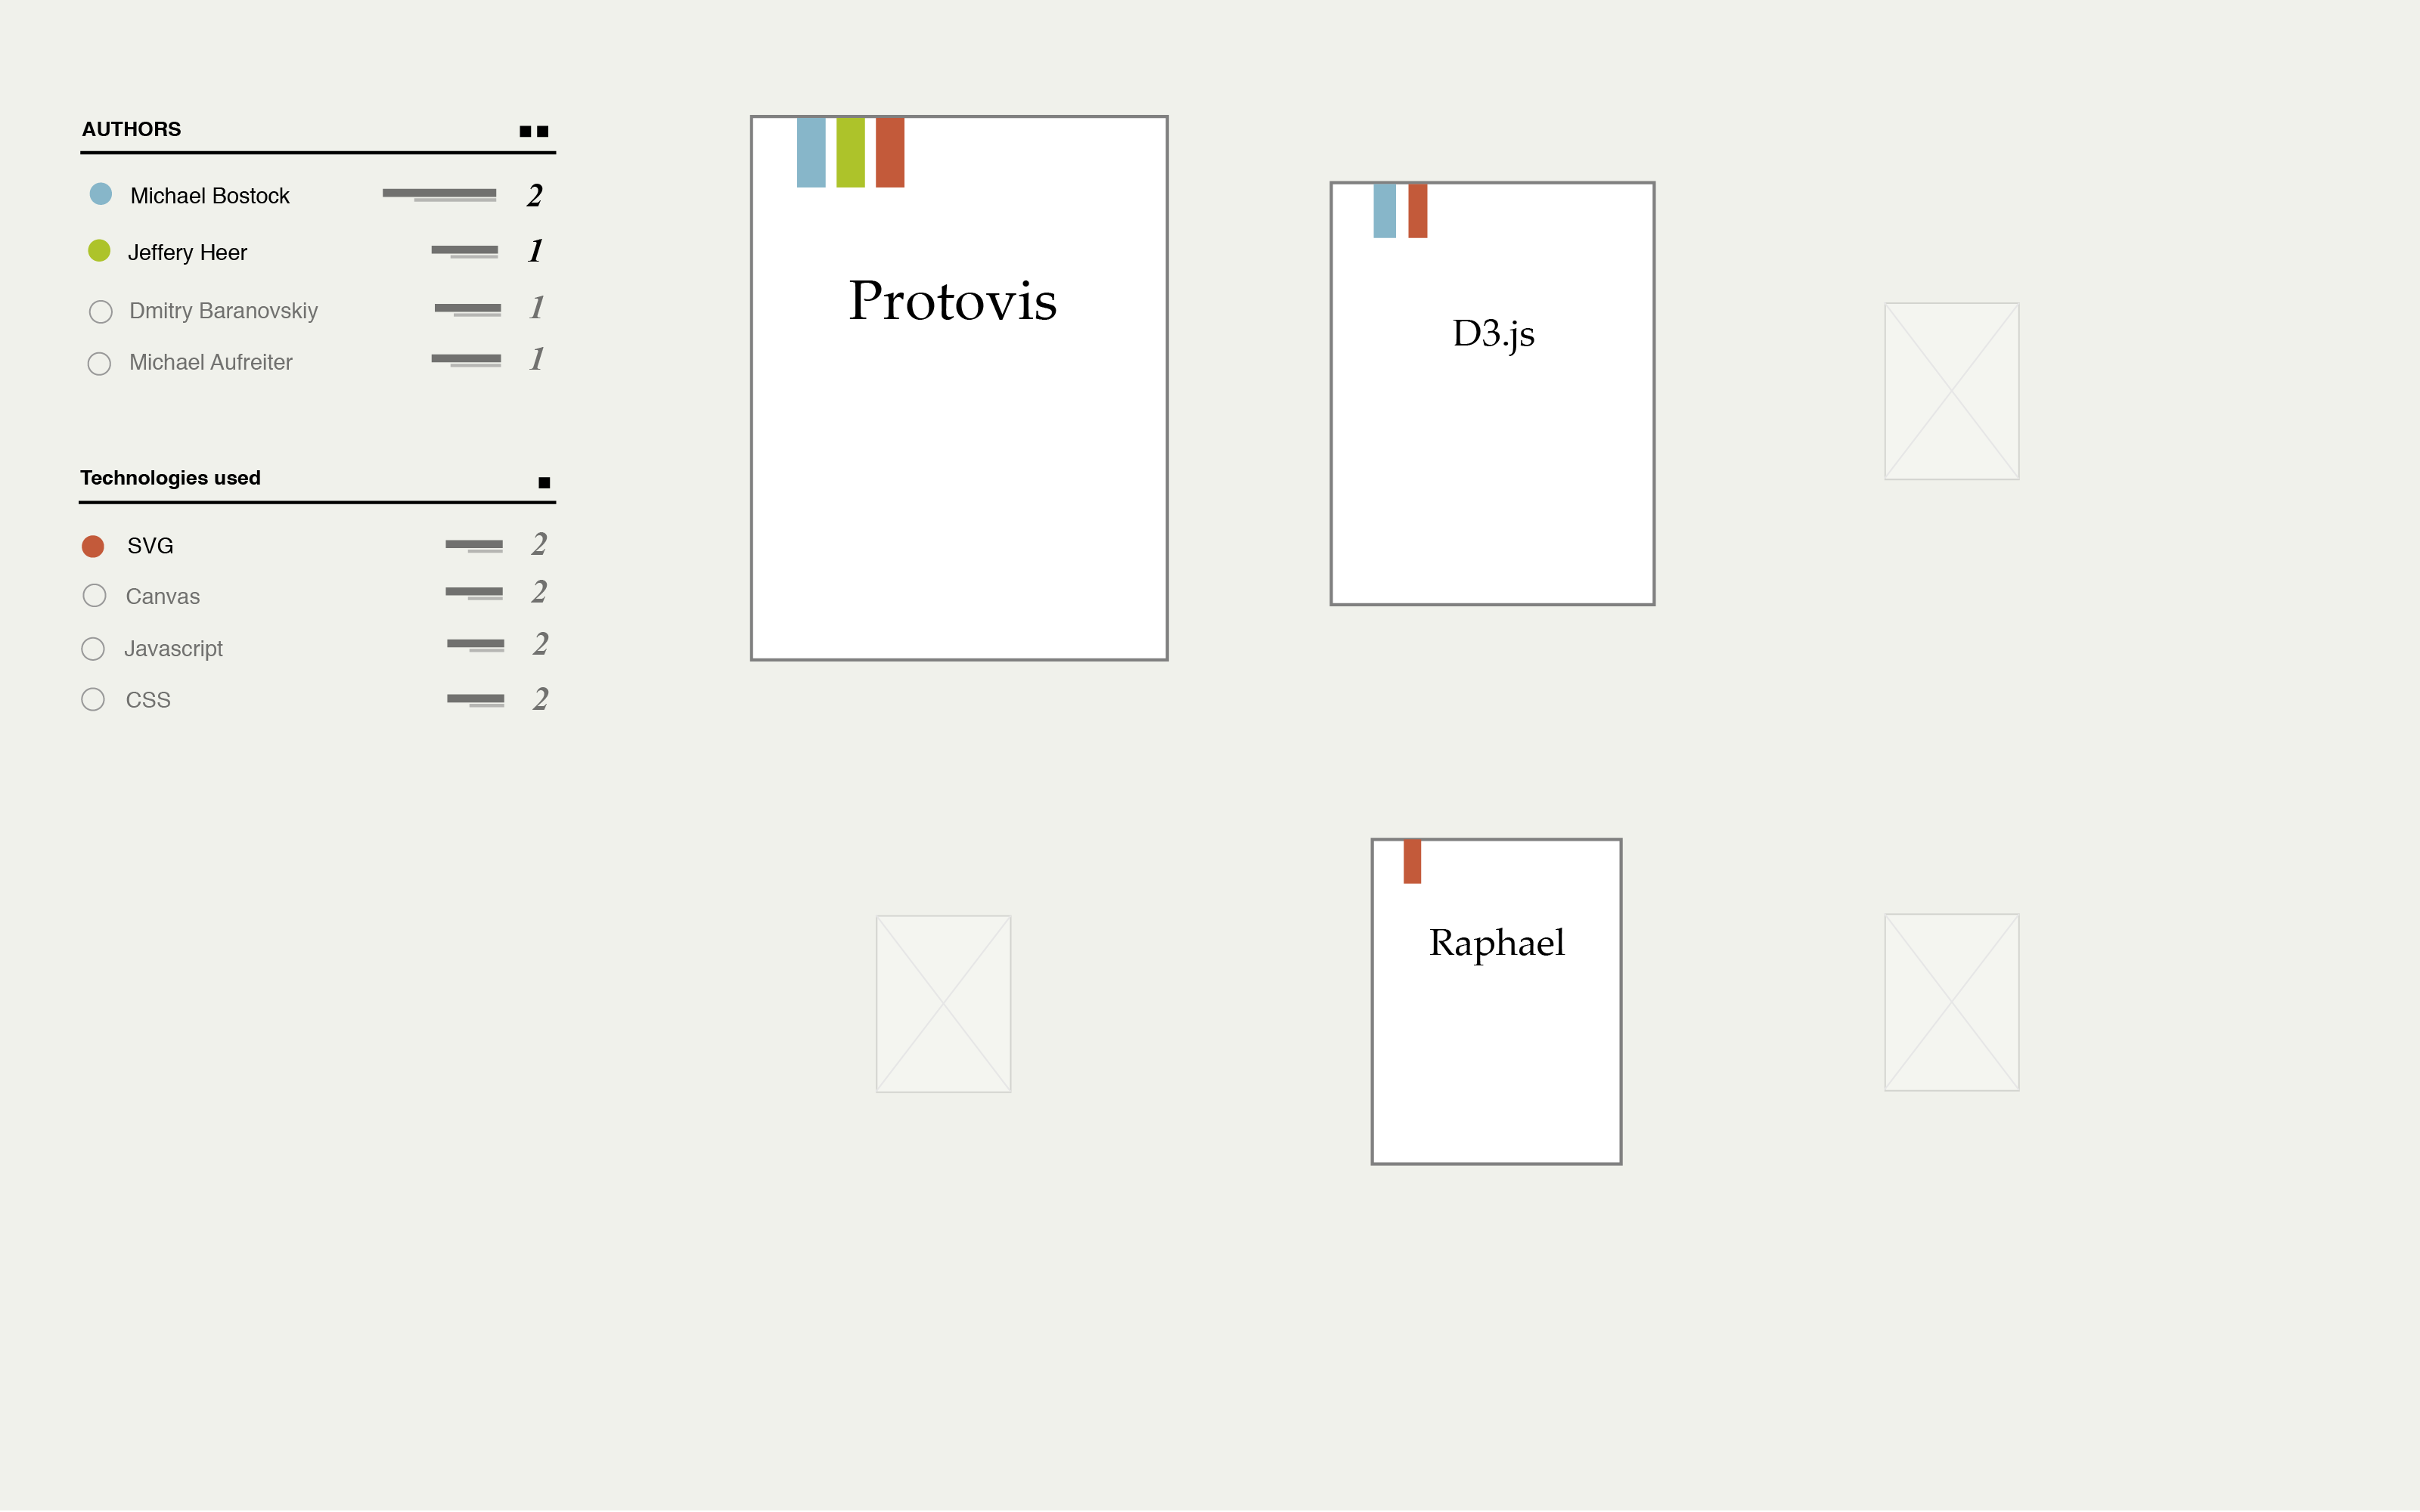
\includegraphics[width=1\textwidth]{doc_explorer/master_thesis_illustrations_2-04}
\caption{Relate: Based on a selection of entities relationships among documents are revealed}
\label{fig:relate}
\end{figure}


\subsection{History}
%%%-----------------------------------------------------------------------------

It is useful to keep a history of actions performed by the user to support \emph{undo}, \emph{replay} and \emph{progressive refinement}. Information Exploration is a task which involves many steps. In order to support the user, it should be possible to retrace the steps performed~\cite{shneiderman96eyes}.


\subsection{Extract}
%%%-----------------------------------------------------------------------------

Based on the current application state, users should be able to store a snapshot of the current context. Later they are either able to restore that context or to share their explorations with others. In a web-based context shareable URL's can be used for state extraction, which is called \emph{View Sharing}~\cite{clark91}.


\section{Data Types}
%%%-----------------------------------------------------------------------------

The following classification by \emph{Data Type}, adapted from Shneiderman \cite{shneiderman96eyes}, is not meant to be seen as strict, but can be helpful to organize visual designs mentally into classes. The \emph{Data Types} described are closely related to how an item of a collection suits a corresponding graphical representation. Based on the explanations of Shneiderman, user problems as well as possible graphical representations are identified for each type.


\subsection{1-dimensional}
%%%-----------------------------------------------------------------------------

% \begin{figure}
% \centering
% 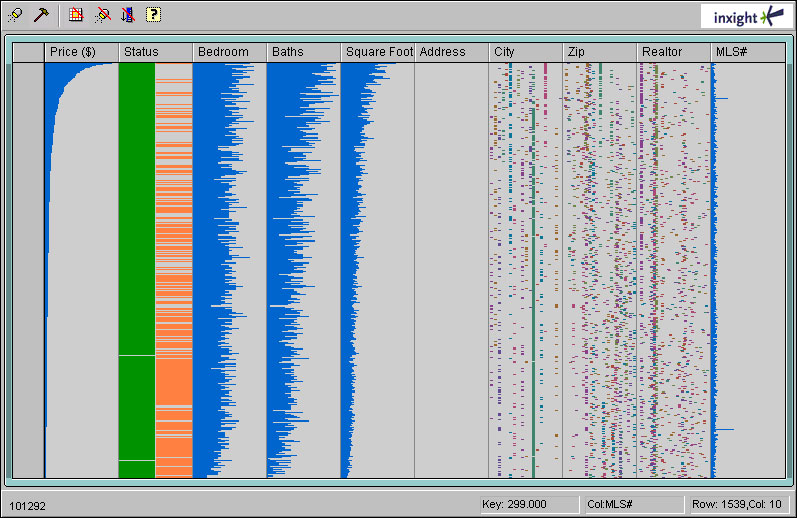
\includegraphics[width=1\textwidth]{tablelens}
% \caption{Table Lens}
% \label{fig:tablelens}
% \end{figure}

1-dimensional data refers to \emph{linear} data types which are organized in a \emph{sequential} manner, such as documents, program source code or an alphabetical list of names~\cite{shneiderman96eyes}. Users usually want to access global information about the characteristics of the data they are viewing as well as how a particular element in the list compares to others. Sometimes users might want to search for specific results within the full dataset based on user defined criteria. This is commonly solved by applying methods for \emph{scrolling} to pick up desired elements. To improve the effectiveness of navigation, compact visual presentations are used, which encode certain properties (such as the number of characters of a line) to represent individual items in the collection.


\SuperPar User problems:

\begin{itemize}
\item Find the total number of items
\item Find items, e.g. a line in a document, that match particular attributes (e.g. if the line is a section)
\end{itemize}


\begin{figure}
\centering
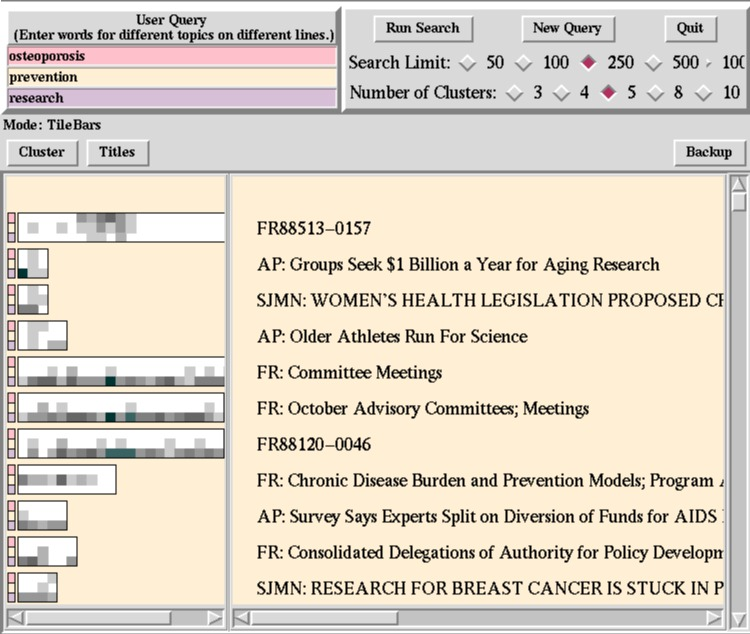
\includegraphics[width=1\textwidth]{tilebars}
\caption{Tilebars visualizing the output of a query to a medical database with three terms: osteoporosis, prevention and research. While Tilebars on the left show relationships between those terms, corresponding documents appear on the right.}
\label{fig:tilebars}
\end{figure}

\SuperPar Examples:

\begin{itemize}
\item \textbf{Tilebars}~\cite{Hearst95tilebars} encode contents of documents using bars. As shown in Figure~\ref{fig:tilebars}, rectangle shading is used to indicate absence or presence of topics within a document.
\item \textbf{The Table Lens}~\cite{tablelens97} is an example for a Bifocal Display~\cite{Spence82} that shows detailed information in focus and less information in the surrounding area.
\end{itemize}


\subsection{2-dimensional}
%%%-----------------------------------------------------------------------------

Planar or map data, such as geographic maps, floor plans or computer chip designs are examples for 2-dimensional data. It is characterized by items in a collection that cover some part of the total area available. A dataset can be considered 2-dimensional if questions about \emph{direction}, \emph{location}, \emph{size} and \emph{distance} can be answered. For a collection of countries including geo information, possible questions could be: How close is Prague to Vienna? How big is Prague compared to Vienna? 2-dimensional data contains a number of attributes that will be used in the visual environment. Examples for such attributes are longitude and latitude, width and height, etc. In reality, all data visualization environments are displayed on a 2D surface, which sometimes leads to confusion regarding classifying data as 2-dimensional.

\begin{figure}
\centering
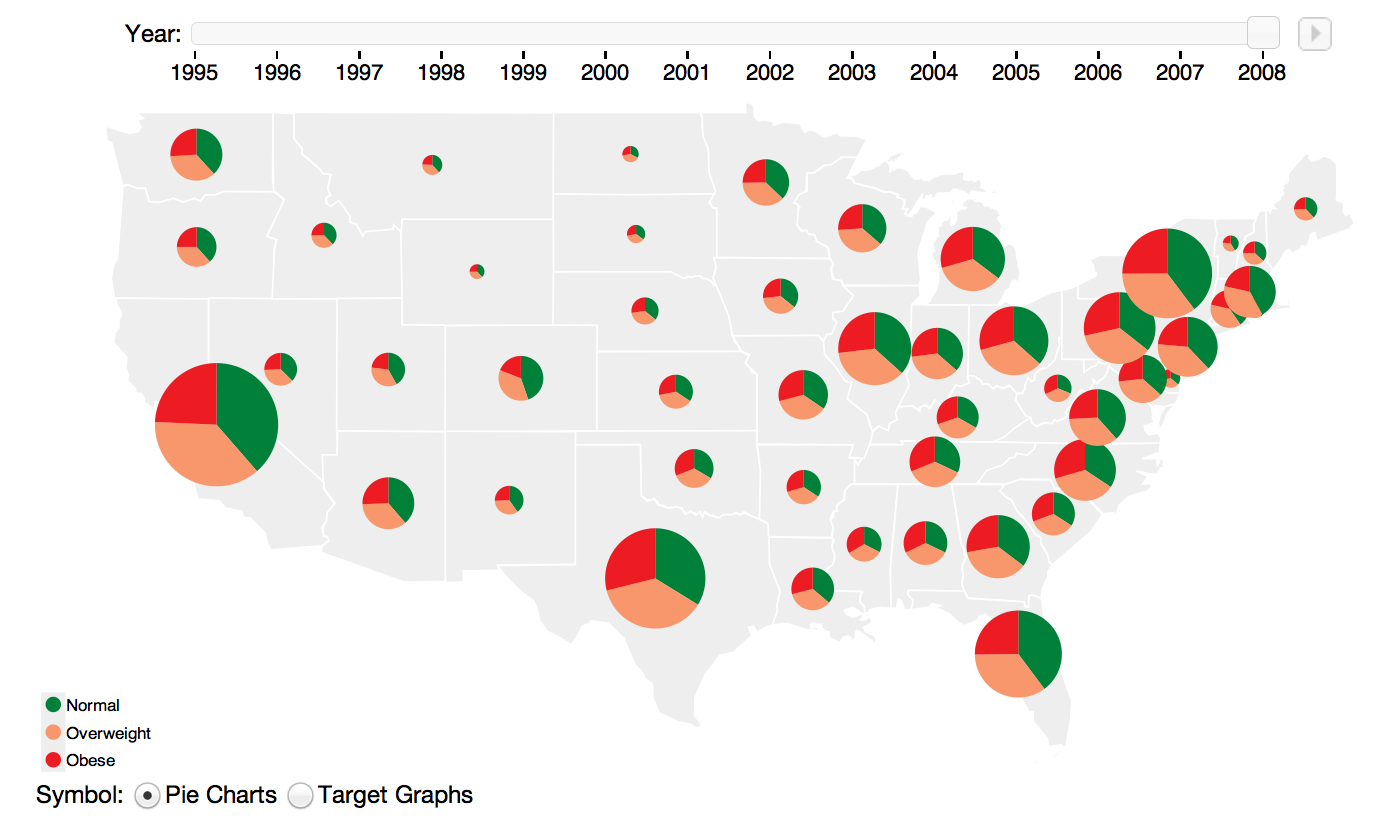
\includegraphics[width=1\textwidth]{map}
\caption{Graduated Symbol Map of Obesity in the U.S., 2008}
\label{fig:map}
\end{figure}

\SuperPar User Problems:

\begin{itemize}
\item Find adjacent items
\item Containment of one item by another
\item Paths between items
\end{itemize}

\SuperPar Examples:

\begin{itemize}
\item \textbf{Graduated Symbol Maps}, as shown in Figure~\ref{fig:map}, place symbols over an underlying map that are used to encode a variable associated with a geographic region~\cite{VisualizationZoo:2010}.
\item \textbf{Cartograms} distort the shape of a geographic region, so that the area directly encodes an associated data variable. Figure~\ref{fig:cartogram} shows a Dorling Cartogram, which represents each geographic region with a sized circle~\cite{VisualizationZoo:2010}.
\end{itemize}

\begin{figure}
\centering
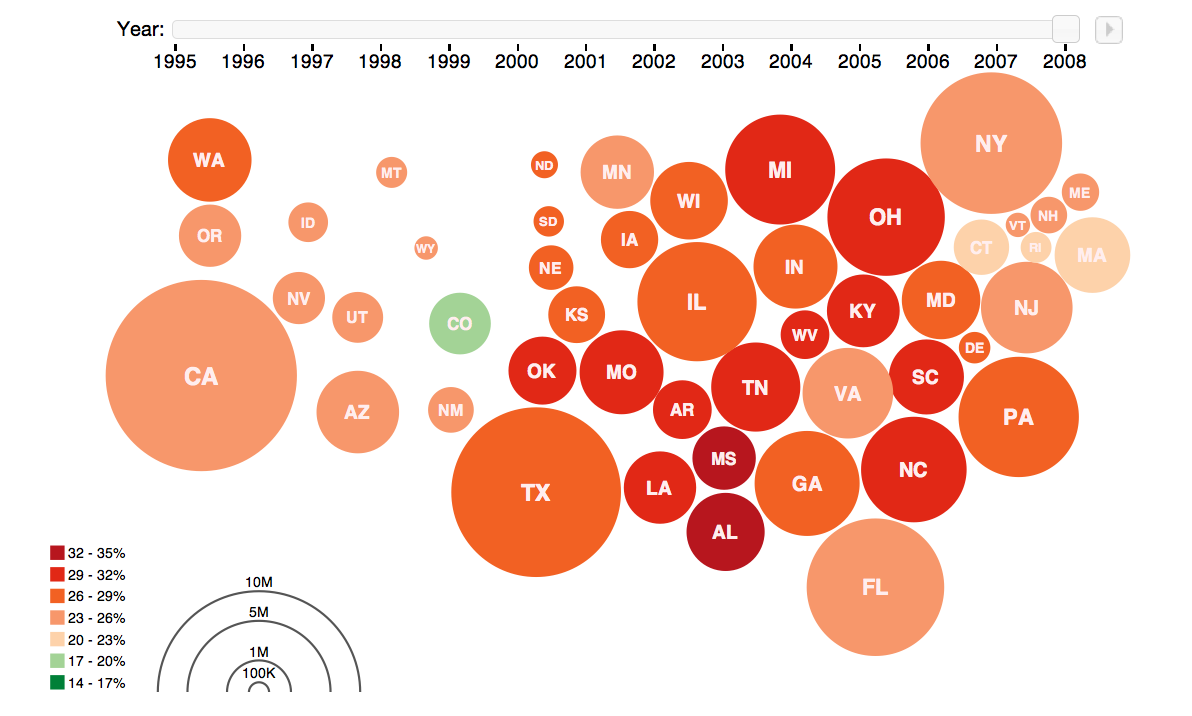
\includegraphics[width=1\textwidth]{cartogram}
\caption{Dorling Cartogram of Obesity in the U.S., 2008}
\label{fig:cartogram}
\end{figure}



\subsection{3-dimensional}
%%%-----------------------------------------------------------------------------

\begin{figure}
\centering
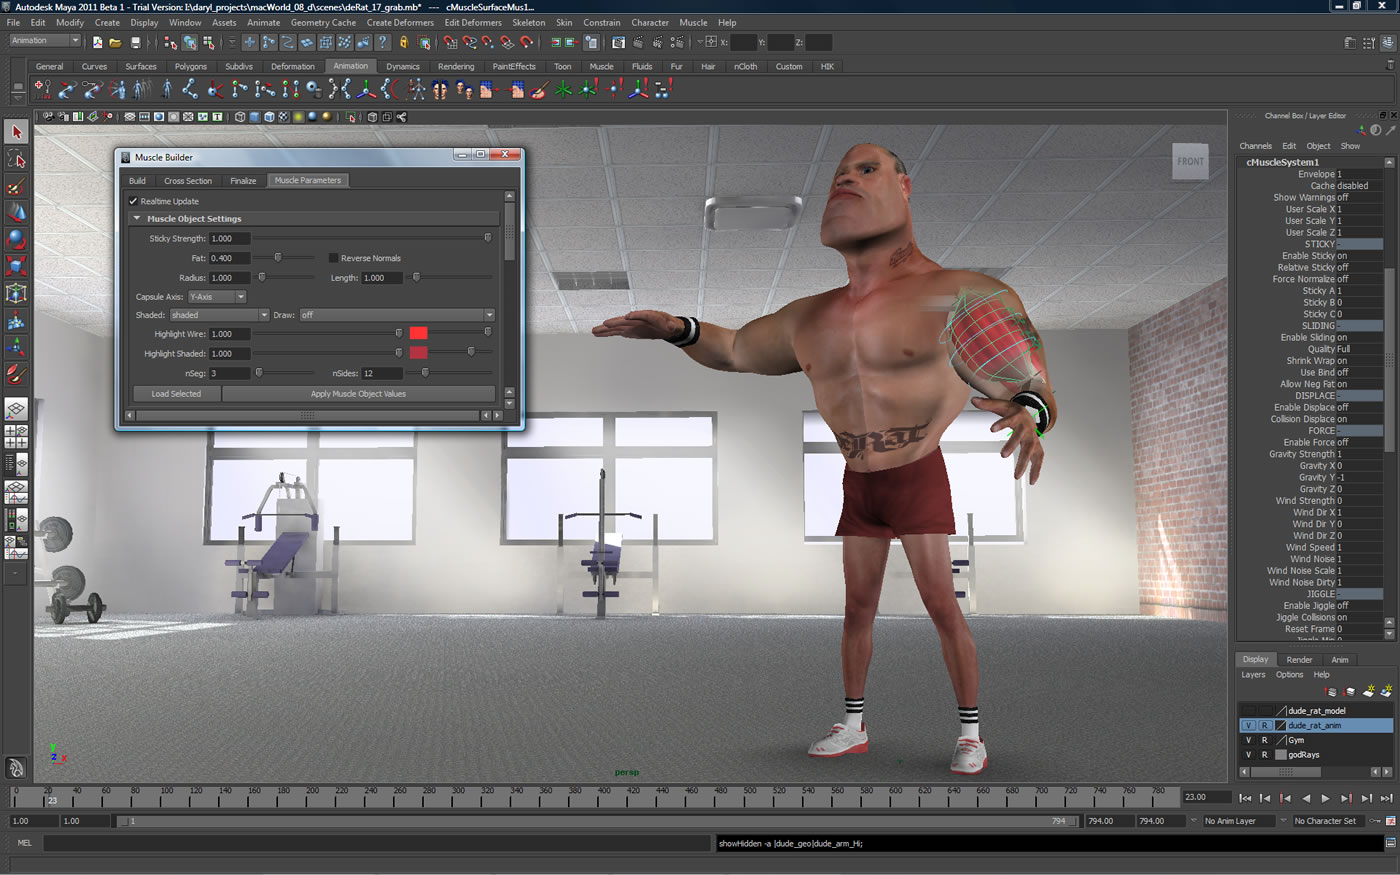
\includegraphics[width=1\textwidth]{maya}
\caption{Autodesk Maya utilized for character animation}
\label{fig:maya}
\end{figure}

3-dimensional data involves real-world objects like landscapes, the human body or buildings. Such objects are typically composed of lower level objects, involving volume and complex relationships between each other~\cite{shneiderman96eyes}. Computer-assisted design systems (CAD) for architects or 3D animation software are designed to handle 3-dimensional relationships. While 3D computer graphics and computer assisted design are employed frequently, Information Visualization in three dimensions is still novel. 3D representation in the context of Information Visualization should be applied with care. If a dataset can effectively be represented in two dimensions, plotting them in 3D space does not add any value. What the presenter creates here has been called ``chart chunk'' by Edward Tufte~\cite{tufte09}.


\begin{figure}
\centering
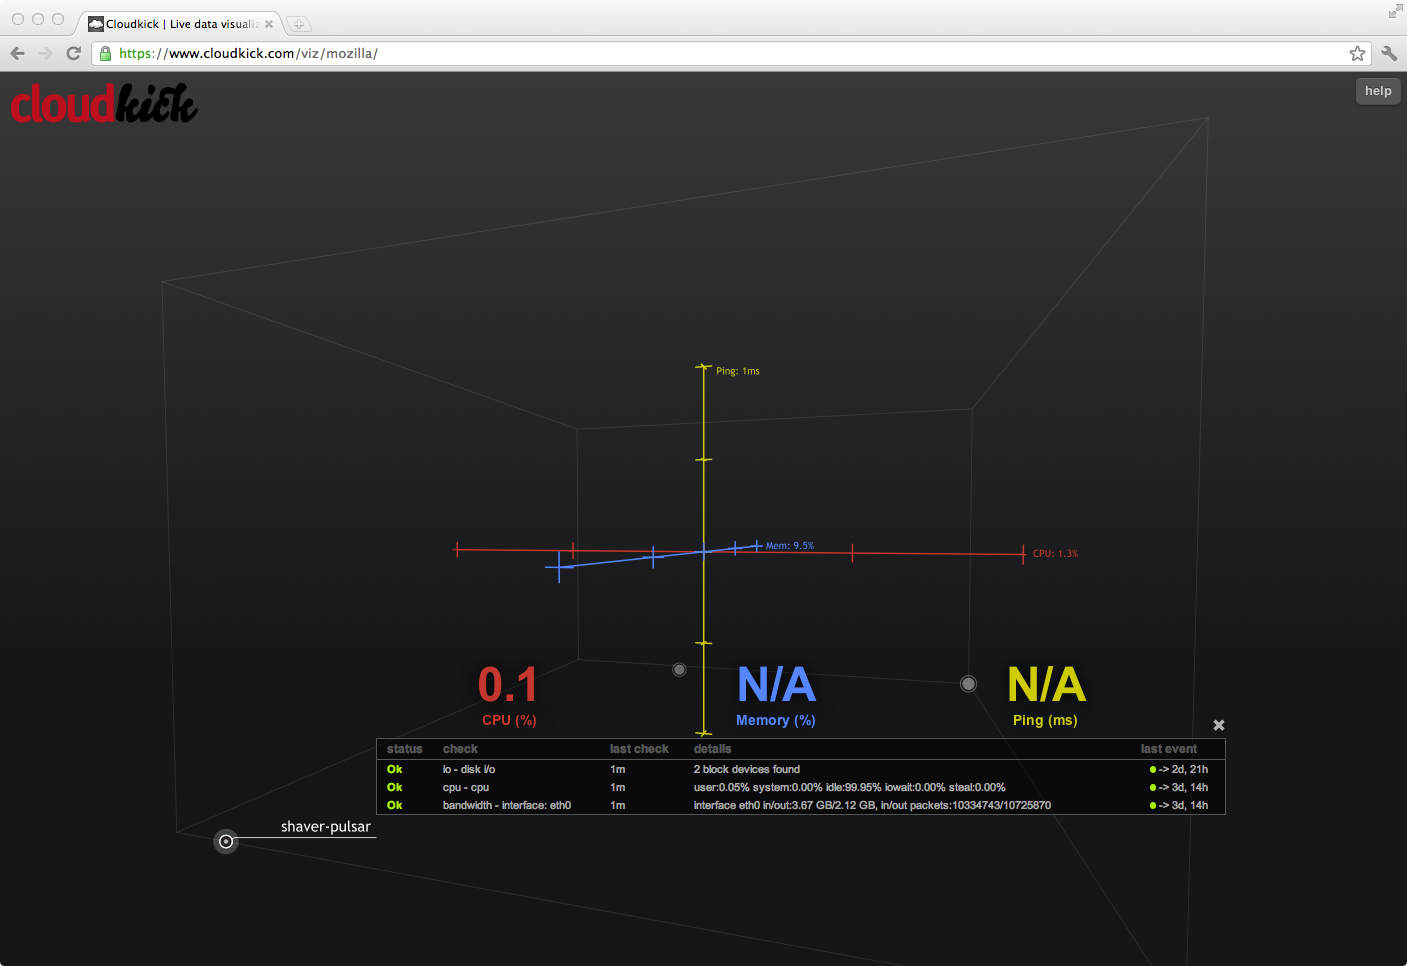
\includegraphics[width=1\textwidth]{cloudkick}
\caption{Cloudkick Vis: Monitored Servers of a cloud infrastructure are plotted in 3-dimensional space, according to performance metrics like CPU usage, Memory usage, and Ping latency.}
\label{fig:cloudkick}
\end{figure}


\SuperPar User Problems:

\begin{itemize}
\item Find adjacent items
\item Understanding the current position and orientation when viewing objects
\item Detecting occlusion
\item Containment issues
\end{itemize}


\SuperPar Examples:

\begin{itemize}
\item \textbf{Autodesk Maya}\footnote{http://usa.autodesk.com/maya}, as shown in Figure~\ref{fig:maya}, is a 3D composition software that provides tools for \emph{animation}, \emph{modeling}, \emph{visual effects} and \emph{rendering}.
\item \textbf{Cloudkick Vis}\footnote{https://www.cloudkick.com/viz/mozilla/} (Figure~\ref{fig:cloudkick}) is a visual server monitoring workspace that displays server status information in realtime.
\end{itemize}


\subsection{Temporal}
%%%-----------------------------------------------------------------------------

Temporal data involves values changing over time and is one of the most common forms of recorded data. Time-varying phenomena are important to many domains such as finance, science and public policy. Time series data often needs to be compared simultaneously and demands suitable visualizations. Shneiderman~\cite{shneiderman96eyes} draws a distinction to 1-dimensional data as soon as data items have a start and finish time (which may overlap).


\begin{figure}
\centering
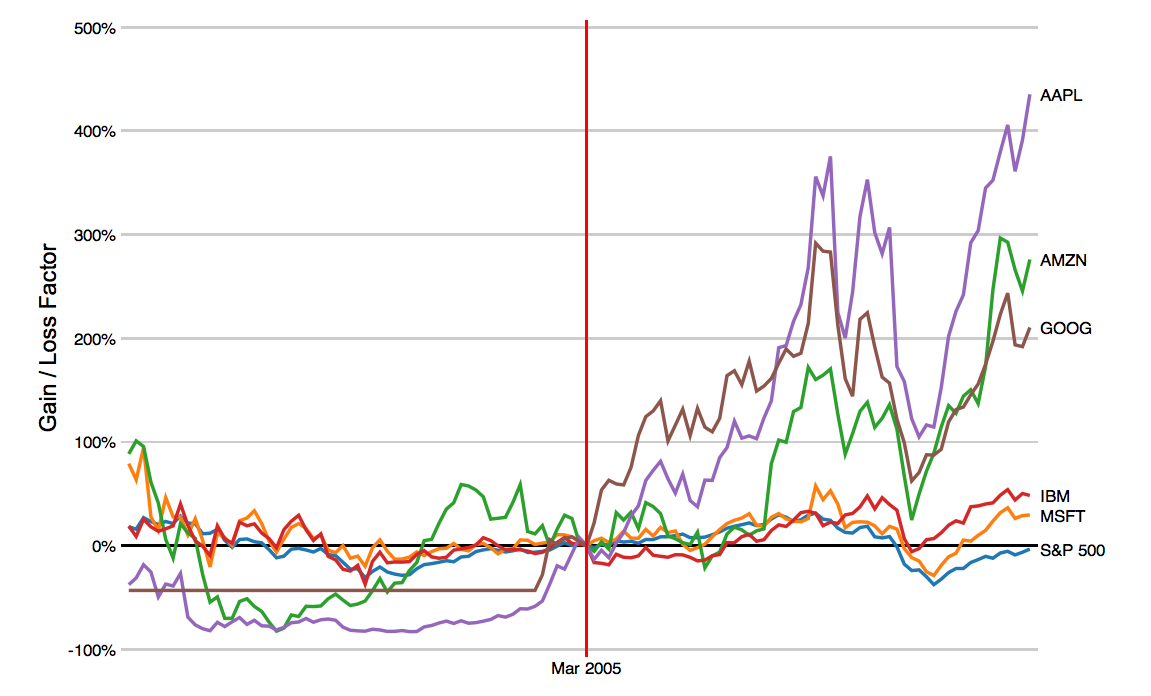
\includegraphics[width=1\textwidth]{timeseries}
\caption{Index Chart of Selected Technology Stocks, 2000-2010}
\label{fig:timeseries}
\end{figure}

\SuperPar User Problems:

\begin{itemize}
\item Get a chronologic overview about events that happened
\item Find events during a specific time period
\end{itemize}

\SuperPar Examples:

\begin{itemize}
\item \textbf{Index Charts} are used to display relative changes over time~\cite{VisualizationZoo:2010}. Figure~\ref{fig:timeseries} shows the gain/loss factors of selected technology stocks.
\item \textbf{Stacked Graphs} show time series as an aggregation by stacking area charts on top of each other~\cite{VisualizationZoo:2010}. As shown in Figure~\ref{fig:stackedgraph}, the result is a visual summation of time-series values.
\end{itemize}


\begin{figure}
\centering
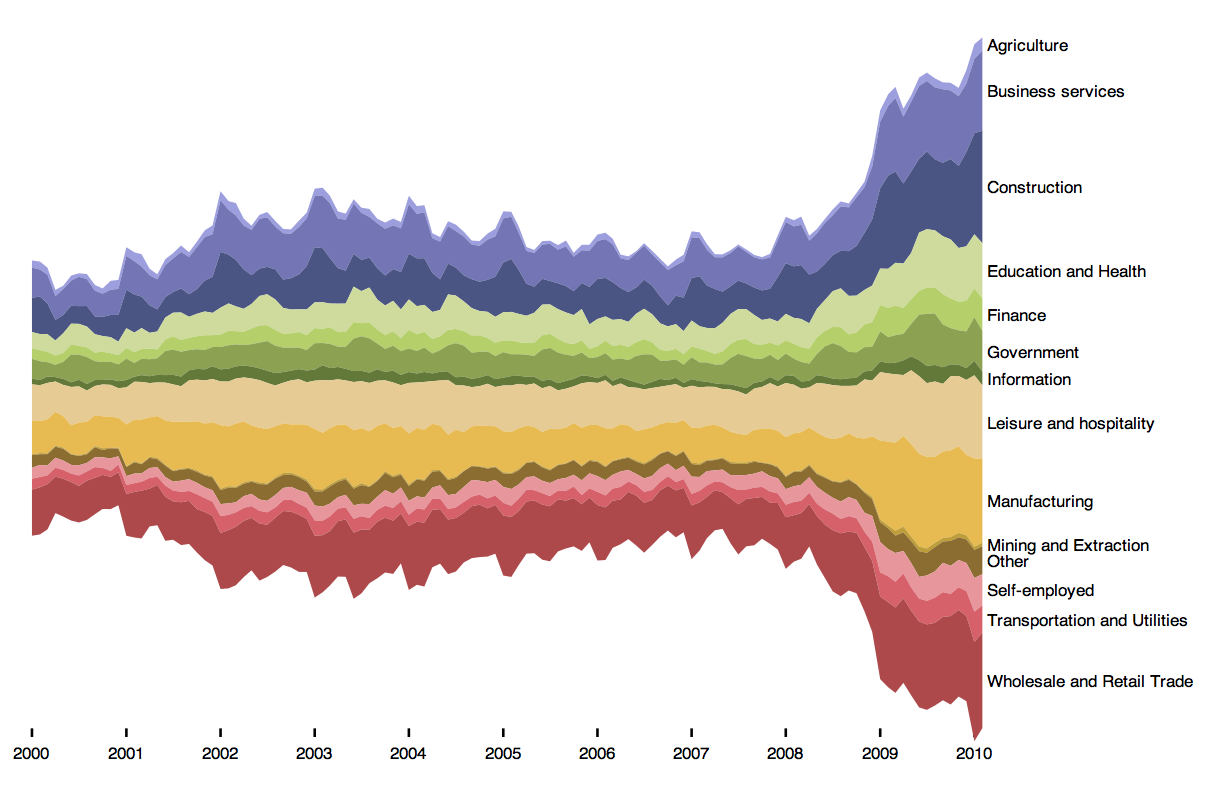
\includegraphics[width=1\textwidth]{stackedgraph}
\caption{Stacked Graph of Unemployment U.S. Workers by Industry, 2000-2010}
\label{fig:stackedgraph}
\end{figure}


\subsection{Multi-dimensional}
%%%-----------------------------------------------------------------------------

\begin{figure}
\centering
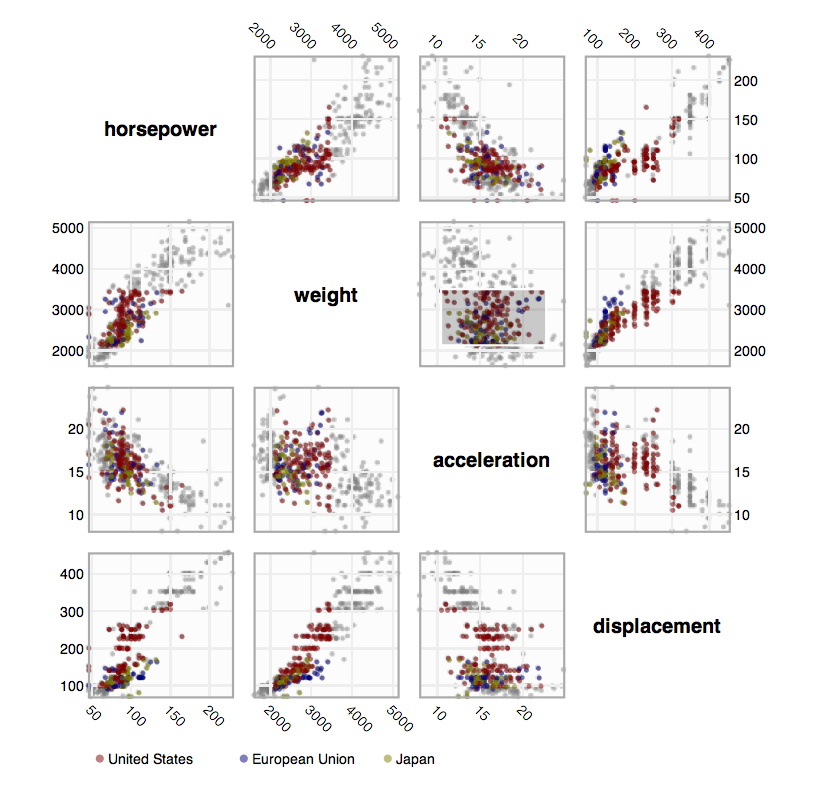
\includegraphics[width=1\textwidth]{scatterplot-matrix}
\caption{Scatter Plot Matrix of Automobile Data}
\label{fig:scatterplot-matrix}
\end{figure}

Multi-dimensional data, characterized by items with n-attributes, occurs frequently and is hard to represent, since it is difficult to picture data mentally in more than three dimensions. An example dataset for this would be a collection of cars, involving multiple numeric attributes such as price, weight, length and speed.

\SuperPar User Problems:

\begin{itemize}
  \item Finding relationships among multiple variables
  \item Finding patterns, clusters, correlations among pairs of variables
  \item Testing hypotheses and predicting future values
\end{itemize}


\SuperPar Examples:

\begin{itemize}
\item \textbf{Scatterplot Matrices} (Figure~\ref{fig:scatterplot-matrix}) enable visual inspection of correlations between any pair of variables~\cite{VisualizationZoo:2010}.
\item \textbf{Parallel coordinates} (Figure~\ref{fig:parallel-coordinates}) plot data on parallel axes and connect corresponding points with lines~\cite{VisualizationZoo:2010}. 
\end{itemize}


\begin{figure}
\centering
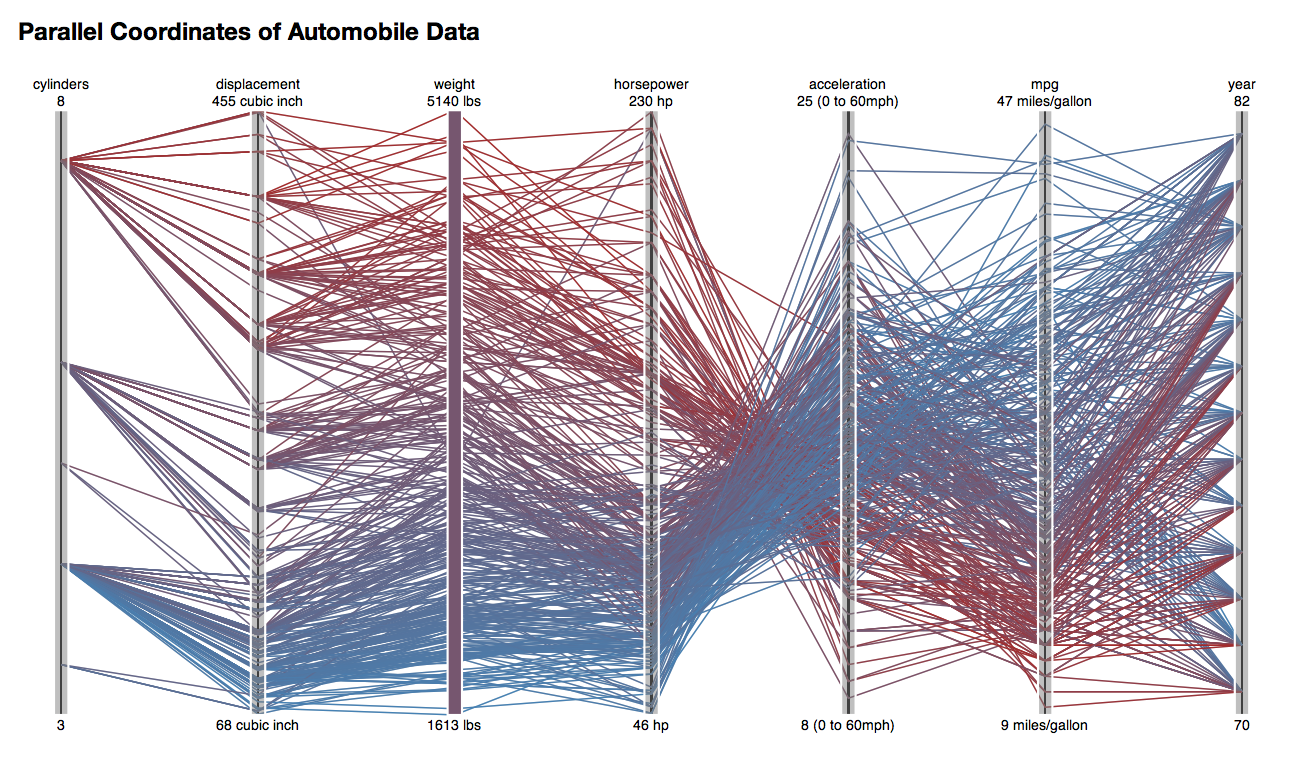
\includegraphics[width=1\textwidth]{parallel_coordinates}
\caption{Parallel Coordinates of Automobile Data}
\label{fig:parallel-coordinates}
\end{figure}

\subsection{Tree}
%%%-----------------------------------------------------------------------------

Tree structures or hierarchies describe parent-child relationships and are composed out of nodes that are connected through links. The topmost node in a tree (which will not have a parent) is called the root node, whereas lower level ones (which have no children) are called leaf nodes. Example tree datasets include spatial entities such as countries, software package hierarchies and genealogies.

\begin{figure}
\centering
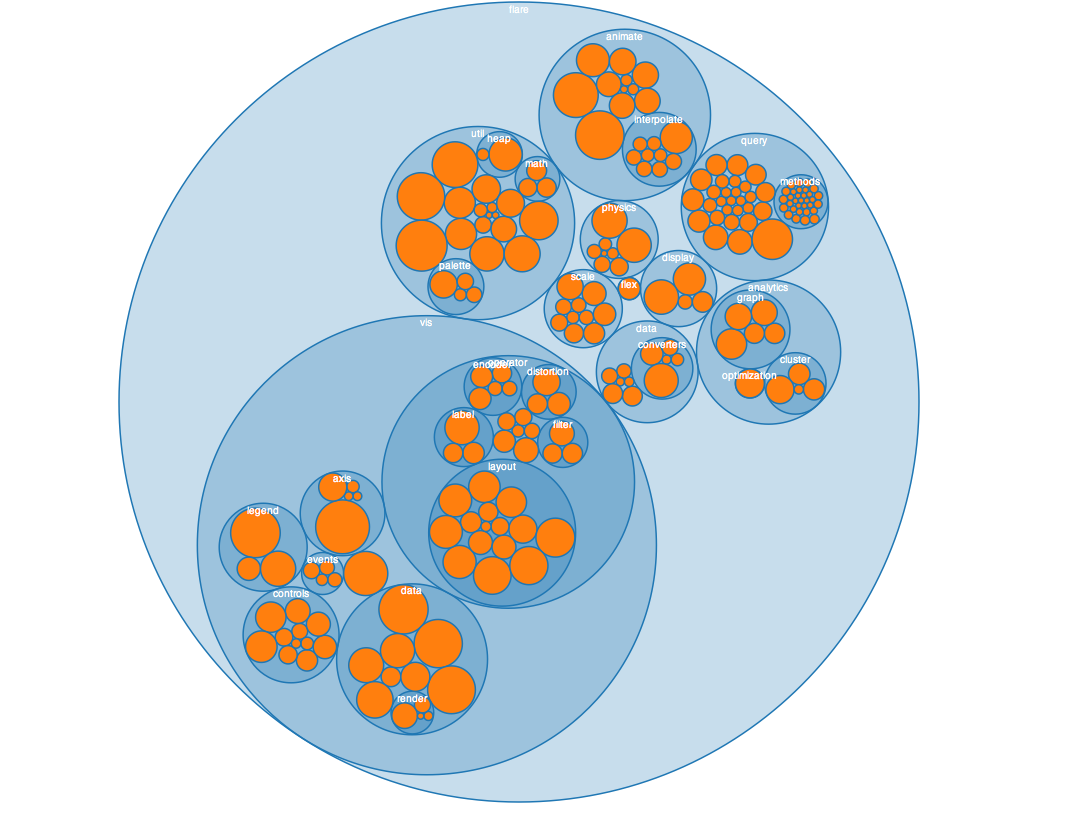
\includegraphics[width=1\textwidth]{nested_circles}
\caption{Nested Circles Layout of the Flare Package Hierarchy}
\label{fig:nested_circles}
\end{figure}


\SuperPar User Problems:

\begin{itemize}
\item How many levels does the tree have?
\item How many children does an item have?
\end{itemize}


\SuperPar Examples:

\begin{itemize}
\item \textbf{Sunbursts} (Figure~\ref{fig:sunburst}) are radial space-filling layouts for tree structures~\cite{VisualizationZoo:2010}.
\item \textbf{Nested Circles} (Figure~\ref{fig:nested_circles}) can also be used to visualize tree hierarchies by employing a \emph{circle-packing algorithm}~\cite{VisualizationZoo:2010}.
\end{itemize}

\begin{figure}
\centering
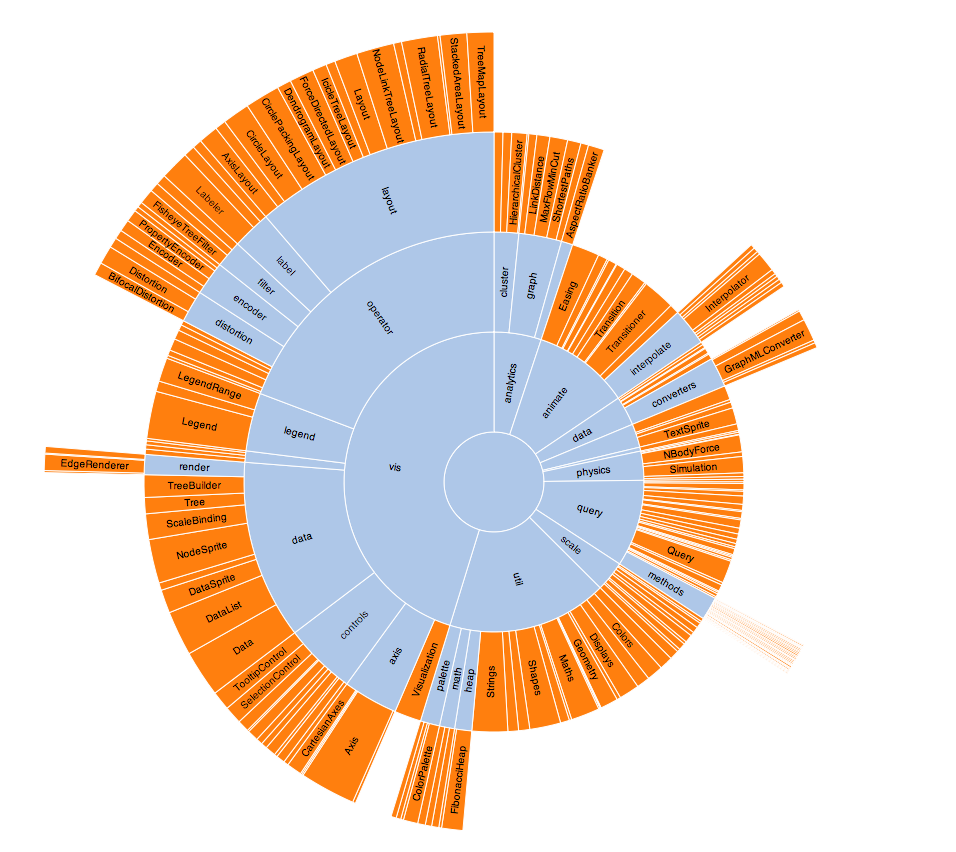
\includegraphics[width=1\textwidth]{sunburst}
\caption{Sunburst Layout of the Flare Package Hierarchy}
\label{fig:sunburst}
\end{figure}


\subsection{Network}
%%%-----------------------------------------------------------------------------

\begin{figure}
\centering
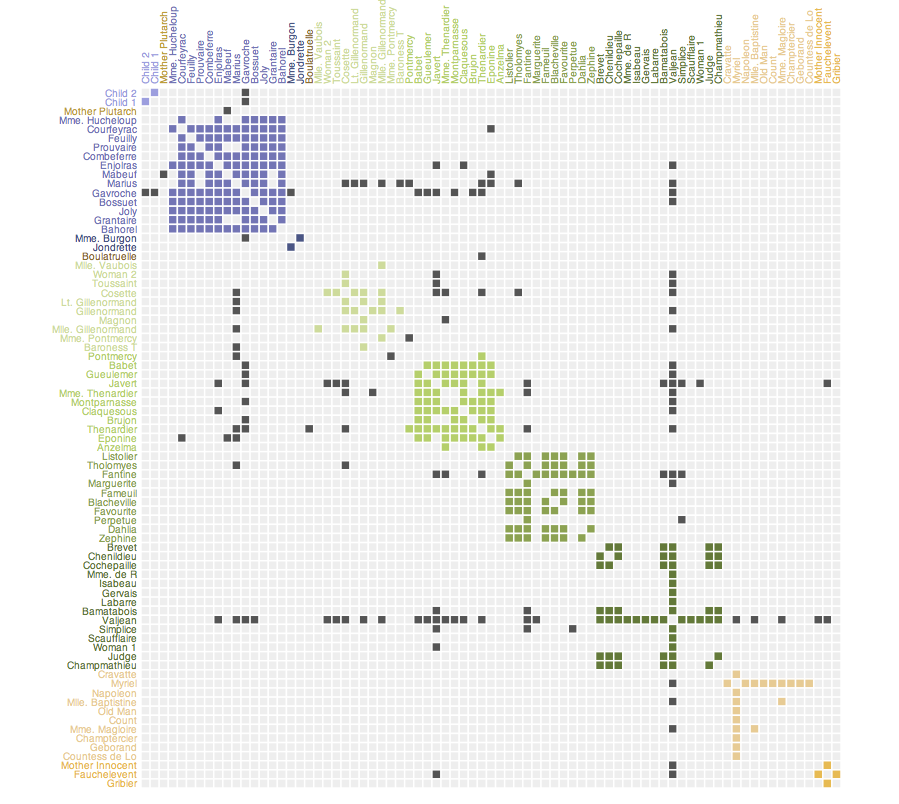
\includegraphics[width=1\textwidth]{matrix-view}
\caption{Matrix View of Les Miserables Character Co-occurrences}
\label{fig:matrix-view}
\end{figure}

One aspect of data that users wish to explore through visualization is \emph{relationship}. Networks are a data structure that capture such relationships using nodes that are connected through edges. Networks are also referred to as graphs in mathematical terminology. Social Networks (who is friend of whom) or workflow descriptions are examples for network datasets. Networks are hard to visualize because of their arbitrary complex structure. The central challenge is the computation of an effective layout, including tasks such as reducing the number of edge-crossings in order to be easily readable by the viewer.

\SuperPar User Problems:

\begin{itemize}
\item Which items are related to a particular item of interest?
\item Which is the shortest or least costly path connecting two items?
\end{itemize}

\begin{figure}
\centering
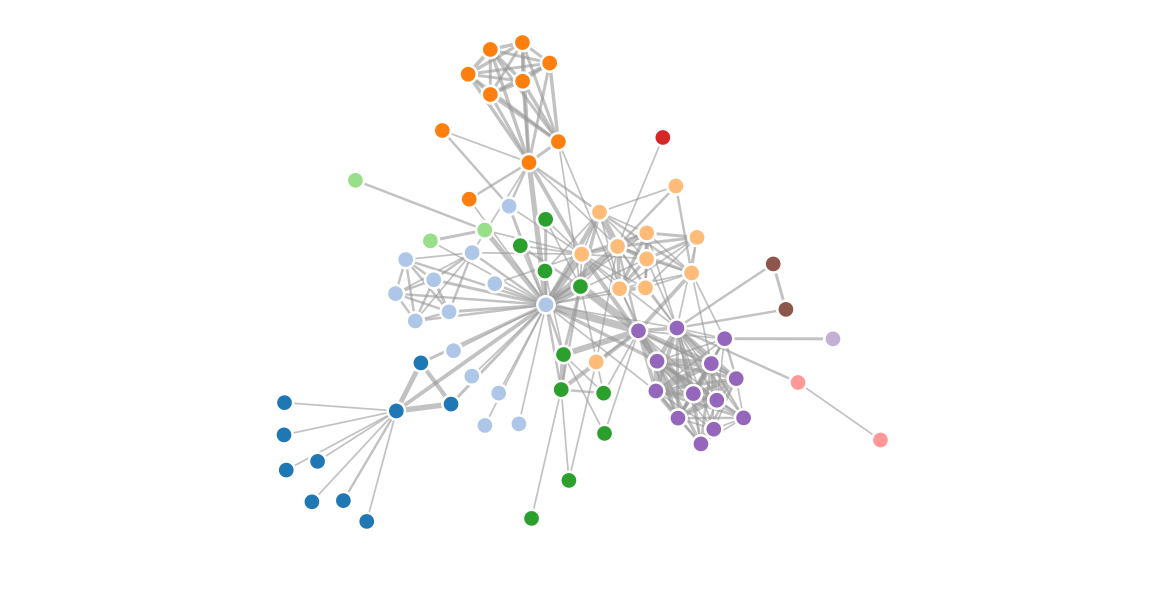
\includegraphics[width=1\textwidth]{force-directed-layout}
\caption{Force Directed Layout of Les Miserables Character Co-occurrences}
\label{fig:force-directed-layout}
\end{figure}

\SuperPar Examples:

\begin{itemize}
\item \textbf{Force directed layouts} (Figure~\ref{fig:force-directed-layout}) are a common approach to network visualization by modeling the graph as a physical system. This is achieved by assigning forces among the set of edges and the set of nodes~\cite{VisualizationZoo:2010}.
\item \textbf{Matrix Views} (Figure~\ref{fig:matrix-view}) represent linked data according to a graph's adjacency matrix.
\end{itemize}


\section{Summary}
%%%-----------------------------------------------------------------------------

The basic concepts of Information Visualization were introduced in this chapter. After taking a look at the \emph{Visualization Process} in general, illustrative examples were used to describe the \emph{Tasks} and \emph{Data Types} of Information Visualization according to Shneiderman~\cite{shneiderman96eyes}. Based on that fundamental knowledge, the next chapter is dedicated to the application of Information Visualization within web-based environments.

\end{english}
\begin{english}

\chapter{Implementing Web-based Visualizations}
\label{cha:web_based_visualization}

Web-based Visualization has a long history in Scientific Visualization and Information Visualization and has seen a recent resurgence in the larger context of social visualization~\cite{Johnson08}. These visualizations have been realized using small applets which are backed by programming environments such as Adobe Flash or Java. With the latest progression of browser technology, these third-party applets are continuously replaced with web-native API's. This chapter gives an overview about techniques and tools available for building interactive web-based visualizations.

According to Bostock and Heer~\cite{Protovis09}, tools used to visualize data are divided into two categories: 
\emph{Visualization Systems} are high-level abstractions that are primarily used for data visualization, whereas \emph{Graphical Systems} operate on low-level graphical primitives. This dichotomy is not meant to be seen as strict. Thus, toolkits may fall somewhere in between.

\section{Graphical Systems}
%%%-----------------------------------------------------------------------------

Low-level graphical systems have a long history in computer science. They are ranging from vector-based drawing programs (e.g. Adobe Illustrator) to low-level rendering API's (OpenGL, Java2D and Processing)~\cite{Protovis09}. Drawing programs aim to improve accessibility and allow designers to manipulate graphical marks in order to build and customize their visualizations. However those drawings are mostly static and demand manual composition by the designer.

In order to support interactive visualizations, which are generated based on live data, the usage of Rendering API's is necessary. In addition to traditional API's (OpenGL, Java2D), modern languages, such as Processing, have been developed to make the process of creating visualizations easier. Processing provides a simplified interface and enables even non-programmers to construct visualizations.

These libraries are general purpose, but typically support only imperative methods for rendering graphical primitives such as ellipses and polygons~\cite{Protovis09}. In response to that, higher-level tools such as Flash and Piccolo were introduced to simplify tasks such as \emph{interaction} and \emph{animation} by providing a \emph{scene graph} abstraction. All those API's do not provide any visualization abstractions, thus tasks such as layouting, interaction, animation (motion-tweening) are left to the user.


\section{Visualization Systems}
%%%-----------------------------------------------------------------------------

According to Bostock and Heer~\cite{Protovis09}, Visualization Systems are tools explicitly designed for the purpose of data visualization. They include common abstractions and mathematical models to make the task of creating interactive visualizations easier. Such tools include support for \emph{data-management}, \emph{layout algorithms}, \emph{interaction}, and \emph{animation}.


\subsection{Consumer Software}
%%%-----------------------------------------------------------------------------

The most widely-used visualization tools are built into consumer software, such as spreadsheet applications like Microsoft Excel or Google Spreadsheets. Such tools typically take tabular data as their input and map it to a visual representation based on a user-selected chart-type. Those tools are easy to use and have broad success, although there are a number of shortcomings, noted by Wilkinson~\cite{wilkinson2005grammar}.
Users only have limited options to adjust the built-in chart types and they cannot introduce new ones. According to Bostock and Heer, due to the high cost of switching tools and the iterative nature of visualization design~\cite{card99}, frequent compromise is likely.

\subsection{Analytical and Exploratory Tools}
%%%-----------------------------------------------------------------------------

A second category are \emph{Analytical and Exploratory Tools}, which are designed to provide flexible options for visual data explorations. A prominent example is Tableau\footnote{http://www.tableausoftware.com/}, which integrates data manipulation with visualization. Tableau allows to adjust queries by interacting with the visual representation. Other approaches, such as Wilkinson's Grammar of Graphics \cite{wilkinson2005grammar}, a dedicated language for specifying visualizations as statistical graphs, offer greater flexibility. Such systems take advantage of meta-data in order to derive appropriate default visual encodings \cite{Bertin83,Mackinlay86automatingthe}.

According to Heer and Bostock, control over graphical output is still limited for these tools. Also, they form closed systems, making them unsuitable for the design of customized domain specific visualizations~\cite{Protovis09}.


\subsection{Programming Toolkits}
%%%-----------------------------------------------------------------------------

The third category identified by Bostock and Heer are \emph{Programming Toolkits}, which are popular for presenting live data or allowing user interaction. While some of them (e.g. Google Chart API\footnote{http://code.google.com/apis/chart/}) only support a number of chart types, thus implying similar trade-offs as consumer software, others are more expressive and extensible (such as the InfoVisToolkit\footnote{http://thejit.org/} or Flare\footnote{http://flare.prefuse.org/}). These tools typically come with a data management framework, coupled with visualization and interaction components.

The InfoVis Toolkit, for example, introduces ``widgets'' that combine visualizations into separate units, which can be extended at any time. In contrast, Prefuse and Flare follow the data state model \cite{Chi98anoperator} and maintain a collection of parametrized visual objects, each associated with data. Using this approach, designers are enabled to specify the properties of visual objects (e.g. position, shape, color) by using configurable operators in order to determine layout and color encoding. 

Protovis~\cite{Protovis09}, the proposed solution by Bostock and Heer, introduces a declarative specification allowing the separation of \emph{specification} and \emph{execution}. The declarative specification is portable, so additional rendering engines such as Java2D or Flash can be targeted in future. Also, this approach should allow the optimization of the visualization pipeline, for example through lazy evaluation of visual properties with large datasets.


\section{Available Technology} % The web as an environment
%%%-----------------------------------------------------------------------------

Although creating graphically intensive applications was already possible with 3rd-party browser plugins, such as Java Applets, Adobe Flash or Microsoft Silverlight, several native visualization methods are available today. These allow the creation of interactive visualizations directly in the browser without requiring any third-party dependencies. This section describes the most important technologies that are available in current web browsers.

\subsection{SVG}
%%%-----------------------------------------------------------------------------

SVG (Scaleable Vector Graphics) is an earlier standard for drawing shapes in browsers recommended by the World Wide Web Consortium (W3C). SVG is a higher level graphical system providing an interface to an underlying scene graph, which is subsequently rendered to a bitmap. Users can manipulate attributes of certain objects by interacting with the Document Object Model (DOM) interface. Once attributes have been changed, SVG can automatically re-render parts of the scene. The SVG API enables events to be associated with objects, so users can bind event handlers to certain events, e.g. when the user clicks on a certain rectangle. The SVG scene graph can be represented in XML, which serves as an exchange format. SVG has a number of built-in simple shapes, such as rectangles and circles. For more complex shapes, users can utilize SVG's path element.

Because SVG can be represented as XML, external editors can be used to design graphical objects, which are composed of primitive SVG-shapes. Those graphical objects can be injected into an existing SVG scene graph, which provides some sort of modularization.

\subsection{HTML5 Canvas}
%%%-----------------------------------------------------------------------------

The Canvas Element is part of the HTML5 specification\footnote{http://dev.w3.org/html5/spec/Overview.html} and allows dynamic, scriptable rendering of 2D shapes and bitmap images. Canvas uses immediate mode rendering with graphical elements drawn as Javascript commands are issued. Canvas is memory efficient, because only the initial data-structures and the rasterized pixels must be stored in memory. Thus, Canvas is able to display a huge amount of objects, while keeping the memory footprint low. An equivalent SVG representation would consume more memory, as each object of the scene graph must be stored. Conceptually, the Canvas API is a lower level protocol and does not offer a scene graph, but a pixel buffer which can be manipulated by the user.

Since Canvas does not maintain graphical objects, hit testing, which is needed for implementing interaction, must be done manually by matching the coordinates of the mouse click with the coordinates of the drawn shape to determine whether it was clicked, or not.


\subsection{Javascript}
%%%-----------------------------------------------------------------------------

The programming language of the web is \emph{Javascript}. While established platforms (e.g. Java, C, C++) provide a vast number of supportive libraries, the availability of such libraries is rather limited for client-side Javascript. In terms of performance, current Javascript implementations are sufficiently fast. Modern browsers even allow parallel processing through WebWorkers. Because of the nature of the language (interpreted, prototypical, functional), it is questionable if the same programming patterns (familiar from classical environments) should be applied. Javascript developers are increasingly preferring declarative interface design to imperative programming style. The expressive power of domain specific languages (DSL) is also realized frequently and fits well into the Javascript programming model \cite{deursen2000}. A DSL is a higher level abstraction focussing on a particular application domain and providing a simplified interface. In the context of Information Visualization, it seems reasonable to apply those modern patterns to visualization toolkits and supportive libraries as well.

\section{Tools Landscape}
%%%-----------------------------------------------------------------------------

Based on recent developments in the field of web-based Information Visualization, a selection of established visualization libraries is introduced. It will be examined which approaches they follow, what type of application they are intended for and how they differ from each other. For illustration, each toolkit will be utilized to construct a simple barchart in order to show differences in usage.


\subsection{Processing.js}
%%%-----------------------------------------------------------------------------

Processing.js is a port of the Processing Visualization Language, originally developed by Ben Fry and Casey Reas. It allows existing Processing code to be executed in a web-based environment, powered by the HTML5 Canvas element. It can be used for specifying visualizations in a classical imperative programming style. In order to support native Processing.js code, which is specified in Java syntax, a source code compilation step is necessary. If a user wants to use a widely-adopted visualization language and be able to execute it on the web, or reuse existing Processing code, Processing.js might be a good choice. However, if visualizations are built from scratch and just target the web-platform for execution, there might be better options. Especially the imposed source-code transformation step might complicate debugging and interacting with web-native API's. Processing.js requires users to specify data-types (this is because it uses Java syntax), which is superfluous as Javascript itself is an untyped prototypal language.

In Processing, users might specify a bar chart as a series of rectangles using a for loop and a call to \texttt{rect()}, which immediately draws a single bar to the canvas:

\begin{verbatim}
int[] data = {1, 1.2, 1.7, 1.5, .7, .3};
for (int i = 0; i < data.length; i++) {
  fill(0, 0, 255);
  rect(i * 25, 200, 20, -data[i] * 80);
}
\end{verbatim}


\subsection{Protovis}
%%%-----------------------------------------------------------------------------

Protovis is an extensible toolkit for constructing visualizations by composing simple graphical primitives. In Protovis, designers specify visualizations as a hierarchy of marks with visual properties defined as functions of data. This representation achieves a level of expressiveness comparable to low-level graphics systems, while improving efficiency (the effort required to specify a visualization) as well as accessibility (the effort required to learn and modify the representation).

Protovis is similar to other graphics libraries such as Java 2D or Processing. It provides a mechanism for drawing rectangles (bars), circles (dots), lines, and polygons (areas). However, Protovis uses a declarative rather than imperative syntax. In contrast to Processing.js, Protovis users almost never use a loop. A set of related graphical elements, such as the bars in a bar chart, are specified as a single mark. The mark is associated with data and the properties are specified as functions, encoding the data graphically:

\begin{verbatim}
vis.add(pv.Bar)
  .data([1, 1.2, 1.7, 1.5, .7, .3])
  .width(20)
  .height(function(d) { return d * 80 })
  .bottom(0)
  .left(function() { return this.index * 25});
\end{verbatim}

\SuperPar When it comes to animation, Protovis allows to specify transitions, but it turned out there are critical limitations. That is why this project was discontinued in favor of D3.js, the official successor of Protovis, which uses a fundamentally different approach, targeting animation and interaction~\cite{D3}.


\subsection{D3.js}
%%%-----------------------------------------------------------------------------

D3 (Data-Driven Documents)~\cite{D3} is a progression of Protovis, developed by its original author, Michael Bostock. Instead of using an execution independent specification language, D3 enables direct inspection and manipulation of a web-native representation: the standard Document Object Model (DOM). With D3, designers selectively bind input data to document elements, which are part of the DOM. They are applying dynamic transforms to do both, generate and modify content. Using an representation transparent approach, expressiveness can be improved and the immediate evaluation of operators simplifies debugging and allows iterative development. The downside of this is that D3 is tied to a specific representation, the DOM, and thus cannot be ported to another rendering engine. D3 was built for the purpose of animation to allow highly interactive and responsive data visualizations. The specification of a bar chart would read as follows:

\begin{verbatim}
var bars = vis.selectAll("g")
    .data([1, 1.2, 1.7, 1.5, .7, .3])
  .enter().append("svg:g")
    .attr("transform", function(d, i) {
      return "translate(" + i*25 + ", 0)"; 
    });
bars.append("svg:rect")
    .attr("width", 20)
    .attr("height", function(d) { return d * 80; });
\end{verbatim}


\subsection{Unveil.js}
%%%-----------------------------------------------------------------------------

Unveil.js, the toolkit developed in the course of this thesis, implements a higher level visualization framework on top of HTML5 Canvas. It introduces graphical objects, adds an API for specifying animations and provides mechanisms to reduce overall CPU consumption. In other words, it tries to unite the advantages of both interfaces, SVG and Canvas. Chapter~\ref{cha:unveil} covers this in more detail.

\begin{verbatim}
var scene = new uv.Scene({
  actors: function() {
    return _.map([1, 1.2, 1.7, 1.5, .7, .3], function(d, index) {
      return {
        type: 'rect',
        x: index * 25,
        y: 200,
        width: 20,
        height: -d * 80,
        fillStyle: 'blue'
      }
    });
  }();
});
\end{verbatim}



\subsection{VVVV.js}
%%%-----------------------------------------------------------------------------

VVVV is a graphical programming environment for prototyping and developing multi-media applications and interactive visualizations. While the original VVVV runs as a desktop application on Windows, VVVV.js\footnote{http://vvvvjs.quasipartikel.at} introduces a web-based runtime environment for VVVV patches. VVVV.js is a work-in-progress, but introduces a novel approach to web-based data visualization. Visualizations are no longer specified as literal source code, but using a visual programming language, expressed through nodes that are connected by input and output pins. Nodes function as independent modules, which take input data, do some processing and yield output data accordingly. The implementation of a node forms a single instruction that operates on multiple data items. In addition to artistic targets, VVVV.js can also be utilized efficiently for creating data visualizations. Figure~\ref{fig:vvvvjs} shows the specification of the barchart example.

\begin{figure}
\centering
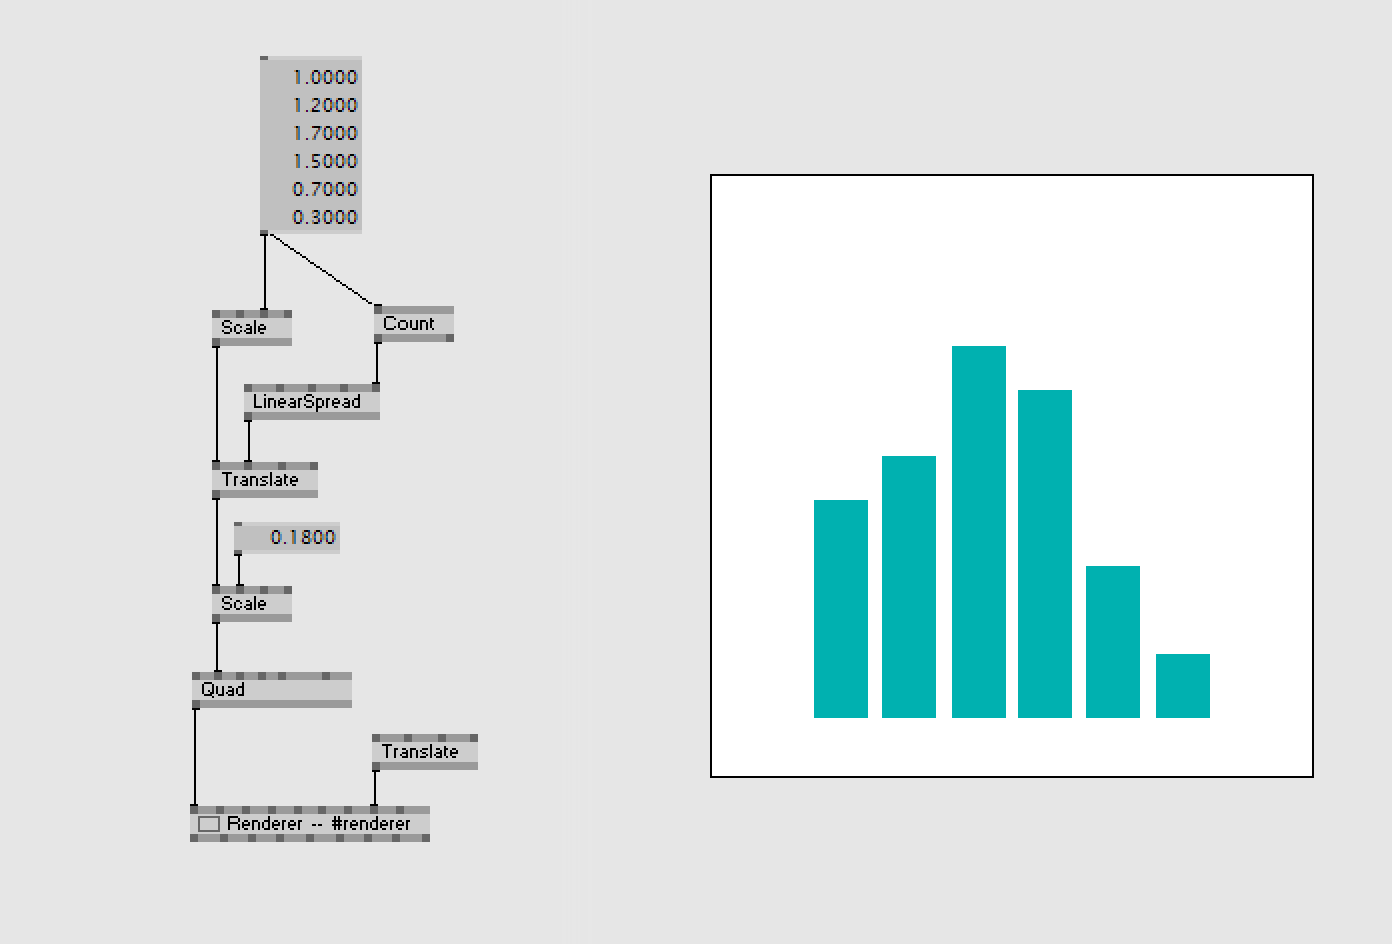
\includegraphics[width=1\textwidth]{vvvvjs}
\caption{VVVV.js used to visually specify a simple Barchart}
\label{fig:vvvvjs}
\end{figure}


\section{Summary}
%%%-----------------------------------------------------------------------------

It is quite hard to choose the right technology for a certain visualization task. If there are huge amounts of data involved, web-native solutions may be exhausted, thus relying on classical environments may remain a better choice. If the requirements on data transmission are suitable for the web, it depends on the task and the favored approach of the developer, which native technology should be utilized. Browsers use different implementations and support different aspects of these technologies. 

However, SVG as well as HTML5 Canvas are thoroughly supported by the majority of current web browsers. After looking at the current range of available toolkits, different approaches were identified such as \emph{toolkit-specific abstraction} vs. \emph{representation transparency} or \emph{imperative programming} vs. \emph{declarative specification}. These are all fundamentally different strategies to approach Information Visualization, each having its own field of application. It is important to understand these differences in order to choose the right tools to build efficient visualizations.

It must also be taken into account that in practice, developers often need to support legacy browsers, that do not support the new interfaces (e.g. Internet Explorer prior to Version 9 does not support the Canvas Element).

\end{english}
\begin{english}

\chapter{Requirements for a Web-based Visualization Toolkit}
\label{cha:requirements}

This section is dedicated to examine what makes a good visualization toolkit. Based on the current state of technology and relevant literature, a set of requirements is identified. The results are taken for the design goals of Unveil.js, the author's attempt to create a visualization toolkit on top of the HTML5 Canvas API.

\section{Declarative Language Design}
%%%-----------------------------------------------------------------------------

The utilization of declarative languages often simplifies programming tasks, which is especially useful for information designers. The idea of declarative languages is that users specify \emph{what} the results of a computation should be rather than \emph{how} the results should be computed. This typically comes along with separating \emph{specification} from \emph{implementation}, which is helpful for language users to focus on their domain-specific application characteristics, while freeing language developers to optimize internal processing~\cite{DeclarativeLD10}. Heer and Bostock name HTML and CSS as very successful representatives of declarative languages as they have enabled millions of novice programmers to develop web-pages. The database query language SQL is another example for utilizing declarative specification to hide the complexity of internals from the user.

According to Heer and Bostock, most existing Information Visualization Toolkits adhere to an imperative programming model which requires visualization design in order to contend with software engineering concerns. Contemporary visualization design tools must deal with an increasing heterogeneity of hardware and interactive devices~\cite{DeclarativeLD10}. Ideally, they should support interfaces ranging from traditional desktop applications to browser based web-clients and multi-touch mobile devices. Furthermore, Visualization Toolkits with the purpose of providing a level of abstraction should be able to benefit from hardware advances without the need of changing the public interface that users interact with. By separating \emph{specification} from \emph{execution}, deployment across heterogeneous platforms becomes possible. This approach forms an efficient alternative to creating a specialized visualization framework for each newly introduced hardware platform.

Protovis, an embedded domain specific language (DSL) for web-based visualizations, demonstrates that a declarative language can simplify visualization specification~\cite{Protovis09}.


\section{Cross-platform Deployment}
%%%-----------------------------------------------------------------------------

One could argue that the web by itself is a cross-platform deployment facility. This is not true, since the implementations of browsers differ. There are multiple options (platforms) to choose from~\cite{DeclarativeLD10}. For the rendering stage, a visualization toolkit could either make use of SVG or HTML5 Canvas. In general, all these technologies can be seen as a work in progress, since new features (sometimes considered experimental, such as hardware acceleration, parallel execution) are introduced continuously. Existing API's such as SVG or HTML5 Canvas are improved on a regular basis. In the future there may be additional options for browser-based rendering. A 3D-context for the Canvas API  is already available, including hardware acceleration. This technology, referred to as WebGL, is already implemented in browsers such as Google Chrome or Mozilla Firefox. Also, in many cases users may want to run their visualization on desktop-based environments as well, ideally without additional specification effort. If toolkits are designed to separate \emph{specification} from \emph{execution}, language designers can immediately add support for new features which are offered by continuously improving browsers.

\section{Optimization}
%%%-----------------------------------------------------------------------------

As Heer and Bostock~\cite{DeclarativeLD10} state, by decoupling \emph{specification} from \emph{implementation} language optimizations can be done without interfering with the work of designers. For a visualization toolkit that follows declarative language design idioms, there are various parts involved, all of which can be optimized independently. These are \emph{runtime compilation} of visualization specifications, \emph{evaluation} and \emph{rendering}. As for rendering, using hardware accelerated graphics usually results in a significant increase in performance.



\section{Data Representation and Transformation}
%%%-----------------------------------------------------------------------------

With respect to Information Visualization, the availability of dedicated data processing frameworks is very important. According to Thomas and Cook~\cite{IlluminatingThePath05}, such frameworks should simplify the task of dealing with domain data and support many dimensions, multi-valued properties for both ordinal types (categorical data) and numeric types as well as object types to model complex relationships.

Data processing frameworks are often included in Visualization Toolkits. Google's \texttt{DataTable}, which is part of their Visualization API\footnote{http://code.google.com/apis/chart/interactive/docs/reference.html}, is an example of such a framework. A \texttt{DataTable} represents a two-dimensional, mutable table of values. For data transformations, users can employ a \texttt{DataView} to make a read-only copy of a \texttt{DataTable}. A \texttt{DataView} may contain a filtered sub-set of the original values, rows and columns. Also grouping operations are possible, where a table of rows can be grouped by specified column values. Values of other columns can be aggregated through aggregator functions such as \texttt{google.visualization.data.max}.

Web-based visualizations should be able to consume live data. Thus, suitable abstract representations for domain data are needed in order to separate data from the visual representation. There is a trend towards data-driven visualizations which do not only use raw data but also meta-information (describing the structure of a dataset). This meta-information can be used to adjust the visual representation based on it. It enables the creation of flexible visualizations, supporting a range of diverging domain data and cover multiple use-cases, which is especially important for the field of Visual Analytics.


\section{Object-oriented Composition}
%%%-----------------------------------------------------------------------------

% citation needed

Employing object-oriented design is especially helpful for composing visualizations. Composition can be seen as the task of \emph{assembling  lower-level objects} (marks) to \emph{higher level compound objects}. Object-oriented design is perfectly suitable for tasks that involve graphics. A visualization can be seen as a \emph{composition of graphical objects}, which are arranged according to the underlying data-items. In a visualization scenario, graphical objects (e.g. the dots of a scatterplot) correspond to real-world objects (e.g. each dot depicts a country). Visualization toolkits should therefore encourage object-oriented thinking, as this helps much during the design process.


\section{Interaction}
%%%-----------------------------------------------------------------------------

According to Spence~\cite{InformationVisualization07}, interaction forms the heart of modern Information Visualization. It enables users to view the corpus of data from different angles. This is needed, since the whole dataset cannot be viewed at once. A visualization toolkit, therefore, needs to have first-class interaction support. This involves specifying behavior which should be executed on certain events. For example, if a user clicks on a particular object the graphical representation should change accordingly (e.g. fade in some details related to the selected object).

\section{Animation}
%%%-----------------------------------------------------------------------------

Since interaction triggers changes to the graphical display, it is important to emphasize the \emph{transition from the old state to the new one}. This is where animation comes into play in order to support smooth transitions that help users to understand what is actually changing. Comprehensive support for animation, thus, is an important requirement for visualization toolkits. They should provide a simple interface for specifying animation behavior and provide means to change the attributes (delay, duration, easing method) of motion tweens.


\section{Extensibility}
%%%-----------------------------------------------------------------------------

In order to support a broad range of use-cases without bloating the core library, Visualization Toolkits should feature a concept for modularization. \emph{Separation of concerns} is important in order to manage the complexity for elaborate visualization tasks. Users of a library, which form a community, should be able to design and maintain independent modules that can easily be reused by others. But not only modularization is important. The possibility of adjusting the library, such as changing the behavior of certain parts as well as extending utility methods, can be of great value.


\section{Summary}
%%%-----------------------------------------------------------------------------

Based on the question what makes a good visualization toolkit, a set of requirements, crucial for the quality of a visualization toolkit, have been identified. In Chapter~\ref{cha:evaluation} the quality of selected toolkits is examined based on these requirements.

\end{english}
\begin{english}

\chapter{Unveil.js: A Data-driven Visualization Toolkit}
\label{cha:unveil}

% \section{Motivation}
%%%-----------------------------------------------------------------------------

As described in Chapter~\ref{cha:web_based_visualization}, the HTML5 Canvas API is a low-level graphical system. It provides a number of drawing methods that can operate on a 2D pixel buffer. The fact that the Canvas API does not track objects implies that dependencies between them are not possible. A visualization's state (including the current set of data and commands issued by the user) can always be projected to a picture. Thus, the whole graphics buffer is refreshed on every frame. Visualization authors do not have to take care which objects need to be redrawn on a certain event. With Canvas, when a state change happens, the impact on the graphical representation is available on the next redraw (frame). If the same approach is be applied with SVG, a lot of DOM manipulation would be necessary, which would result in poor performance. On the other hand, building complex visualizations without any kind of abstraction requires a lot of manual work and even leads to poor performance, if not optimized by hand.

Unveil.js is designed to combine the best of both worlds and introduces a slim \emph{layer of abstraction}, namely a \emph{Scene} interface that can be populated with graphical objects, the so called \emph{Actors}. It offers a simple programming interface for creating, updating and removing objects from the scene.

Unveil.js is an open source effort\footnote{http://github.com/michael/unveil} and is released under the MIT license.


\section{Goals}
%%%-----------------------------------------------------------------------------

Unveil.js is dedicated to Information Visualization and was built with respect to the following assumptions:

\begin{itemize}
\item
  In most visualization scenarios the graphical display stays the same in periods where no interaction takes place.
\item
  Most interactive visualizations feature transitions from one state to another.
\end{itemize}

\SuperPar Accordingly, most visualizations do not change state permanently. During periods when the state stays the same, there is no need for redraws. If there was a mechanism that detects state changes and triggers renderings on demand, the Canvas API could be used in very efficient ways. This would allow the creation of smooth animations involving a lot of moving objects while keeping the CPU utilization low, if no animation or interaction takes place.

There are a few considerations that need to be made. Interaction (like mouse movement) can trigger state changes. In cases where animation takes place, there must be subsequent re-renders on a high frame rate in order to make the transitions appear smoothly. Unveil.js implements a concept called \emph{Automatic Frame Rate Determination}. Based on the current state of the visualization, the frame rate can either be zero (no updates), low (during mouse interaction) or high (when animation is happening). Experiments have shown that by using this approach CPU consumption can be reduced remarkably. Compared to SVG the memory consumption is also kept low.

Unveil.js advocates a one-way dependency between input data and the resulting output image. Visualizations should be built in a way that every change of the internal state is immediately reflected on the output side. Using this approach, users do not have to deal with manual partial updates, a tedious and error-prone task. Unveil.js is considered to be a lightweight toolkit that helps managing complexity rather than being a full-featured graphical visualization library. It was designed to meet the following requirements:

\begin{itemize}
\item
  \textbf{Object-oriented} in terms of thinking in graphical objects and modularizing code.
\item
  \textbf{Declarative} in terms of using, configuring and combining existing Actors (graphical objects) and to attach them to the Scene.
\item
  \textbf{Data-driven} to support a two-step mapping of data to an resulting image, involving an analytical abstraction and the transformation to visual objects.
\item
  \textbf{Data Abstractions} for representation and manipulation of domain data.
\item
  \textbf{Multiple Output Displays} for creating independent views on an abstract scene definition.
\item
  \textbf{Automatic Frame Rate Determination} to reduce overall CPU consumption.
\item
  \textbf{Dynamic Properties} allow functions to be used as property values, which are evaluated during runtime.
\item
  \textbf{Interaction support} for mouse picking, zooming and panning.
\end{itemize}


\section{Specifying a Scene}
%%%-----------------------------------------------------------------------------

With Unveil.js, new visualizations are created by constructing a \texttt{Scene} object.

\begin{verbatim}
var scene = new uv.Scene();
\end{verbatim}

\subsection{Actors}
%%%-----------------------------------------------------------------------------

Once the \texttt{Scene} object is ready, users can start adding \texttt{Actors}. An Actor can be a primitive graphical object (like a bar, a line, etc.) or a higher level object, which combines lower level ones (e.g. a snowman that is composed of three circles). Actors typically take graphical properties in their constructor. However, for higher level objects users probably want them to be constructed with \emph{real domain data} instead of graphical oriented properties (width, height, etc.). Users can decide on their own how they want to shape the interface of certain Actors.

\SuperPar The following code creates a bar instance, which will eventually be attached to the scene:

\begin{verbatim}
var bar = new uv.Bar({
  id: 'outer_bar',
  x: 30,
  y: 50,
  width: 30,
  height: 80,
  fillStyle: 'darkblue'
});
\end{verbatim}

\SuperPar Each actor can hold any number of child actors, so another bar will be attached as a child to the parent bar.

\begin{verbatim}
bar.add(new uv.Bar({
  id: 'inner_bar',
  x: 50,
  y: 20,
  width: 20,
  height: 80,
  fillStyle: 'lightblue'
}));

scene.add(bar);
\end{verbatim}

\SuperPar The x and y coordinates are relative to the parent object. Thus, an object itself does not know where it is located in the coordinate-space. It just renders itself relative to the position of its parent. The positioning is done through \emph{matrix transformations}, where for each object the current context \emph{transformation matrix} (context) is calculated on every frame, which conforms to the functionality of a \emph{Scene Graph}.

\subsection{Output Displays}
%%%-----------------------------------------------------------------------------

Before a scene can be started, a display (or drawing surface) needs to be specified:

\begin{verbatim}
scene.display({
  container: 'plotarea',
  width: 800,
  height: 300,
  zooming: true,
  paning: true
});
\end{verbatim}

\SuperPar Unveil.js uses an abstract scene (world-coordinates) that can be projected to one or many displays (canvas elements), which have a local coordinate system on their own. Each display can be modified (e.g. zoomed, paned) independently, which conforms to a view transformation in computer game engines (camera analogy). Once a display is set up, scenes can be started by calling the \texttt{start()} method.

\begin{verbatim}
scene.start();
\end{verbatim}

\SuperPar The scene automatically refreshes attached displays appropriately (on every frame), which implies that performance may decrease if multiple output displays are used.

\subsection{Implementing Custom Actors}
%%%-----------------------------------------------------------------------------

In addition to pre-implemented Actor types, users are encouraged to implement their own Actors suitable to their needs. In Unveil.js the creation of new actors forms a fundamental part of the \emph{Visualization Creation Process}.

\SuperPar In order to illustrate this, here is how the Bar Actor is implemented:

\begin{verbatim}
uv.Bar = function(properties) {
  uv.Actor.call(this, _.extend({
    width: 30,
    height: 50,
    strokeWeight: 2,
    strokeStyle: '#000',
    fillStyle: '#ccc'
  }, properties));
};

uv.Bar.prototype = Object.extend(uv.Actor);
\end{verbatim}

\SuperPar Every Actor inherits from \texttt{uv.Actor} and defines its own properties. In the case of \texttt{uv.Bar}, there is \texttt{width}, \texttt{height}, \texttt{strokeWeight}, \texttt{strokeStyle}, etc. Each Actor needs to know how it can draw itself. This is specified by the \texttt{draw} method that sticks on the Actor's prototype.

\begin{verbatim}
uv.Bar.prototype.draw = function(ctx) {
  ctx.fillRect(0, 0, this.p('width'), this.p('height'));
};
\end{verbatim}

\SuperPar Actors can not only form graphical objects but carry some state (e.g. domain data or user input) which is stored within the object. Such higher level objects can encapsulate behavior (like interactivity or animation) as well.


\subsection{Interaction}
%%%-----------------------------------------------------------------------------

Interaction is a key-feature of modern visualizations. Therefore, Unveil.js aims to provide an abstraction for implementing interaction on Actors. Unlike in SVG, Canvas API users cannot attach event handlers to shapes directly. Instead, users need to detect on their own, i.e. which objects are currently under the cursor. Usually this is done by employing some math, but there is a simpler approach that utilizes the \texttt{isPointInPath()} method provided by the Canvas API. With \texttt{isPointInPath()}, users can check if the current mouse-position is inside the current working path. To support interaction, Unveil.js requires Actors to be equipped with an additional \texttt{drawMask()} method.

\begin{verbatim}
uv.Bar.prototype.drawMask = function(ctx) {
  ctx.beginPath();
  
  ctx.moveTo(0, 0);
  ctx.lineTo(this.properties.width, 0);
  ctx.lineTo(this.properties.width, this.properties.height);
  ctx.lineTo(0, this.properties.height);
  ctx.lineTo(0, 0);
};
\end{verbatim}

\SuperPar This simply draws an invisible rectangle. If there are more complex objects, e.g. star-shapes, a rectangle (also known as a bounding-box) can be used as well to add interaction-awareness. All Actors that have a \texttt{drawMask()} implementation can be easily checked against the current cursor position. For completeness, here is the corresponding code that is used internally to perform the actual hit testing.

\begin{verbatim}
uv.Actor.prototype.checkActive = function(ctx, mouseX, mouseY) {
  if (this.drawMask && ctx.isPointInPath) {
    this.drawMask(ctx);
    if (ctx.isPointInPath(mouseX, mouseY))
      this.active = true;
    else
      this.active = false;
  }
};
\end{verbatim}


\subsection{Event Handlers}
%%%-----------------------------------------------------------------------------

Given that interaction is supported for a certain actor, users are able to bind event handlers to certain events.

\begin{verbatim}
scene.get('inner_bar').bind('mouseover', function() {
  this.p('fillStyle', 'red');
});
\end{verbatim}

\SuperPar This example causes the inner bar to be colored red when the user's mouse cursor enters the object.

\subsection{Dynamic Properties}
%%%-----------------------------------------------------------------------------

Properties can not only takes values but also functions. During rendering, these functions are evaluated dynamically and their return value is taken as the property value.

\SuperPar Instead of specifying a mouseover handler to highlight certain objects, one could also use a dynamic property.

\begin{verbatim}
scene.get('inner_bar').p('fillStyle', function() {
  return this.active ? 'red' : 'darkblue';
});
\end{verbatim}


\subsection{Animation}
%%%-----------------------------------------------------------------------------

% maybe also suitable for the requirements section
In the context of Information Visualization, animation is often utilized in conjunction with state transitions. In other words, when the inner state (either data or user settings) changes, animation can be used to emphasize the transition from one state to another.

Based on new data, a visualization might assign new values to graphical objects, but wants to have this value interpolated over time, from the old value to the new value. Unveil.js users can call the \texttt{animate} method on Actors for that. The first parameter is a hash that contains the new property values. The second parameter determines the animation's duration, whereas the third parameter is optional and can be used to specify an easing function, which should be used for interpolation.

\begin{verbatim}
bar.animate({height: 50}, 2.5, uv.Tween.Easing.Expo.EaseInOut);
\end{verbatim}

% Rendering depends on the current visualization state. As soon as interaction takes place or an animation gets started, subsequent re-renders get triggered automatically.

\subsection{Automatic Frame Rate Determination}
%%%-----------------------------------------------------------------------------

In order to spare CPU cycles, Unveil.js implements a \emph{Frame Rate On-demand Mechanism} to determine the current image refresh rate. This rate is either zero (idle mode) or high (during animation or interaction). It basically works like a semaphore, where each animation that is started increments a counter that keeps track of running frame rate requests. Once the animation has finished, this counter is decremented again. Interaction like mouse movement also increments that counter and decrements it after some time of inactivity. Unveil.js then triggers high-frequent redraws as soon as the counter exceeds zero.

\subsection{Matrix Transformations}
%%%-----------------------------------------------------------------------------

While most often specifying properties (x, y, scaleX, scaleY, rotation) on the Actor suffices, there may be cases where users need more control. For that purpose, Actors expose a so called \emph{Modification Matrix}, which can be directly modified by the user. Working with transformation matrices is a powerful tool and already common practice in game development and graphical programming.

\SuperPar For example, to scale and rotate around a given point in the coordinate system, a series of matrix transforms can be specified.

\begin{verbatim}
var b = new uv.Bar({...});
// move the coordinate system to the desired point
b.translate(40,40);
// scale around this point (= new origin)
b.scale(1.5, 1.5);
// rotate 45 degrees
b.rotate(Math.PI/4);
// move the coordinate system back
b.translate(-40, -40);
\end{verbatim}

\SuperPar To calculate the resulting transformation matrix for drawing, it is initialized with the values of the specified properties and then multiplied with
the modification matrix.

\section{Data Abstractions}
\label{cha:dataabstractions}
%%%-----------------------------------------------------------------------------

Unveil.js was built with a very data-centric approach in mind, offering a number of data abstraction utilities users can use for representing and manipulating domain data. For all data-related concerns Unveil.js relies on Data.js, which is available as a separate library. Data.js is actively maintained and provides a range of features such as queries, filtering, clustering and serializable (thus exchangeable) data-formats. Tabular data can be represented through a \texttt{Data.Collection} interface, whereas complex linked data fits into the \texttt{Data.Graph} model. Not only data but also schema information can be inspected by the user, which can help building even more flexible data-driven visualizations. This can particularly be helpful for implementing \emph{Contextual Data Transformation} functionality, as described by Viegas et. al \cite{manyeyes}.

Here is an example of a \texttt{Data.Collection} containing real-world data about countries.

\begin{verbatim}
var countries_data = {
  "properties": {
    "name": {"name": "Country Name",
      "type": "string", "unique": true },
    "official_language": {"name": "Official Language",
       "type": "string", "unique": true },
    "population": { "name": "Population",
       "type": "number", "unique": true },
    "gdp": { "name": "GDP per capita",
      "type": "number", "unique": true }
  },
  "items": {
    "at": {
      "name": "Austria",
      "official_language": "German",
      "population": 8356700,
      "gdp": 39.761
    },
    "de": {
      "name": "Germany",
      "official_language": "German",
      "population": 82062200,
      "gdp": 46.860
    },
    "usa": {
      "name": "United States of America",
      "official_language": "English",
      "population": 310955497,
      "gdp": 36.081
    }
  }
};
\end{verbatim}

\SuperPar The collection shown above not only holds data for certain countries, but also contains meta-information, expressed as properties. As described in Chapter~\ref{cha:web_based_visualization}, this can be particularly useful for analytical and exploratory visualization tools. 

\begin{verbatim}
languages.at(0).get('name'); // => "German"
languages.at(0).get('population') // => 90418900
languages.at(1).get('population') // => 310955497 for "English"
\end{verbatim}

\subsection{Property Inspection}
%%%-----------------------------------------------------------------------------

Using the Property Inspection API, users can ask a certain property about its type, a human readable name or if it is unique (holding just one value) or not (holding a list of values).

\begin{verbatim}
countries.properties().get('population').type; // => 'number'
countries.properties().get('population').unique; // => false
countries.properties().get('population').name; // => 'Population'
\end{verbatim}

\subsection{Aggregation}
%%%-----------------------------------------------------------------------------

Presumed that a user is interested in the populations grouped by language, the \texttt{Data.Collection.group()} method can be utilized. In order to aggregate the values of population, an aggregator function such as \texttt{Data.Aggregators.SUM} can be used.

\begin{verbatim}
var languages = countries.group(["official_language"], {
  "population": {
    aggregator: Data.Aggregators.SUM, 
    name: "Total Population"
  }
});
\end{verbatim}

\section{A Data-driven Bar Chart}
%%%-----------------------------------------------------------------------------

In the following example, some real world domain data is used, namely countries containing information about their population and GDP per capita. These a visualized in a bar chart (Figure~\ref{fig:bars}). Users will be able to switch between different properties, triggering an animation from the old state to the new one. 

\SuperPar The countries example from Section~\ref{cha:dataabstractions} will be used as a data-source.

\begin{verbatim}
var countries = new Data.Collection(countries_data);
\end{verbatim}

\SuperPar The property that should be visually encoded is determined by the user using a select-box control. The HTML generated looks as follows:

\begin{verbatim}
<select id="property">
  <option value="population">Population</option>
  <option value="gdp">GDP per capita</option>
</select>
\end{verbatim}

\begin{figure}
\centering
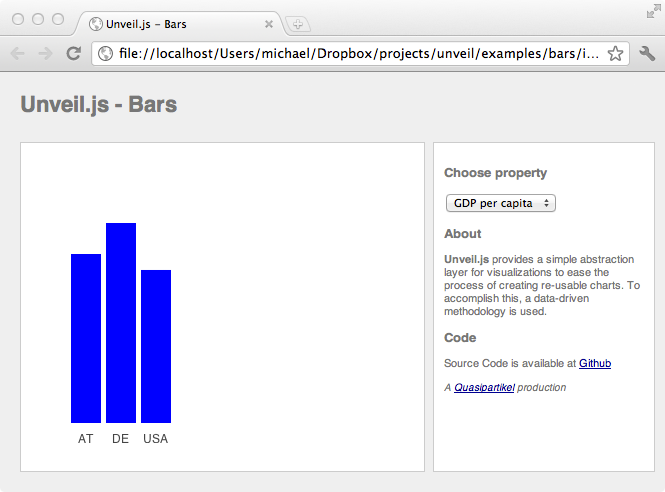
\includegraphics[width=1\textwidth]{bars}
\caption{A data-driven barchart generated from domain data expressed as a \texttt{Data.Collection}}
\label{fig:bars}
\end{figure}

\SuperPar Furthermore, a Scene object is created complete with a specified output display:

\begin{verbatim}
var scene = new uv.Scene({
  displays: [{
    container: 'canvas',
    width: 300,
    height: 300
  }]
});
\end{verbatim}

\SuperPar In order to guarantee that the bars fit on the available screen space, they need to be normalized accordingly. The function shown below maps values from an input domain (real numbers) to an output range (pixels).

\begin{verbatim}
function y(val) {
  var dMax = countries.properties().get(property)
              .aggregate(Data.Aggregators.MAX),
      oMax = 200;
  return parseInt(val/dMax * oMax);
}
\end{verbatim}


\SuperPar The scene will be initialized by adding a bar per data element in the collection. The height property encodes the value of the property under investigation.

\begin{verbatim}  
countries.items().each(function(c, key, index) {
  scene.add({
    id: "country_"+key,
    type: 'rect',
    x: 50+35*index,
    y: 280,
    width: 30,
    height: -parseInt(y(c.get(property)), 10),
    fillStyle: function() {
      return this.active ? 'orange' : 'blue'; 
    },
    interactive: true,
    actors: [
      {
        type: 'label',
        x: 15,
        y: 20,
        width: 30,
        height: 20,
        text: function() { return c._id.toUpperCase() },
        textAlign: 'center',
        fillStyle: '#444'
      }
    ]
  });
});
\end{verbatim}

\SuperPar Additionally, the visualization should allow dynamic switching between properties. For that purpose, property inspection features provided by Data.js are used to find out which numeric properties are available for the collection. By doing so, the visualization can be used with arbitrary collections, even if their structure differs.

\begin{verbatim}
countries.properties().each(function(p) {
  if (p.type === "number" && p.unique) {
    var option = $('<option value="'+p.key+'">'+p.name+'</option>');
    $('#property').append(option);
  }
});
\end{verbatim}

\SuperPar Every time the user selects a property, the bars need to be updated accordingly. In an event handler we are using the \texttt{animate()} method to specify an animated transition of the bar's height.

\begin{verbatim}
function update() {
  property = $('#property').val();
  countries.items().each(function(c, key, index) {
    scene.get("country_"+key).animate({
      height: -parseInt(y(c.get(property)), 10)
    }, 1.0);
  });
}
$('#property').change(update);
\end{verbatim}

\SuperPar Finally, the scene can be started.

\begin{verbatim}
scene.start();
\end{verbatim}


\section{Example Applications}
%%%-----------------------------------------------------------------------------


There is a range of examples available, that show different applications of Unveil.js. For each of them, the source code is available for inspection.

\subsection{Scatterplot}
%%%-----------------------------------------------------------------------------

\begin{figure}
\centering
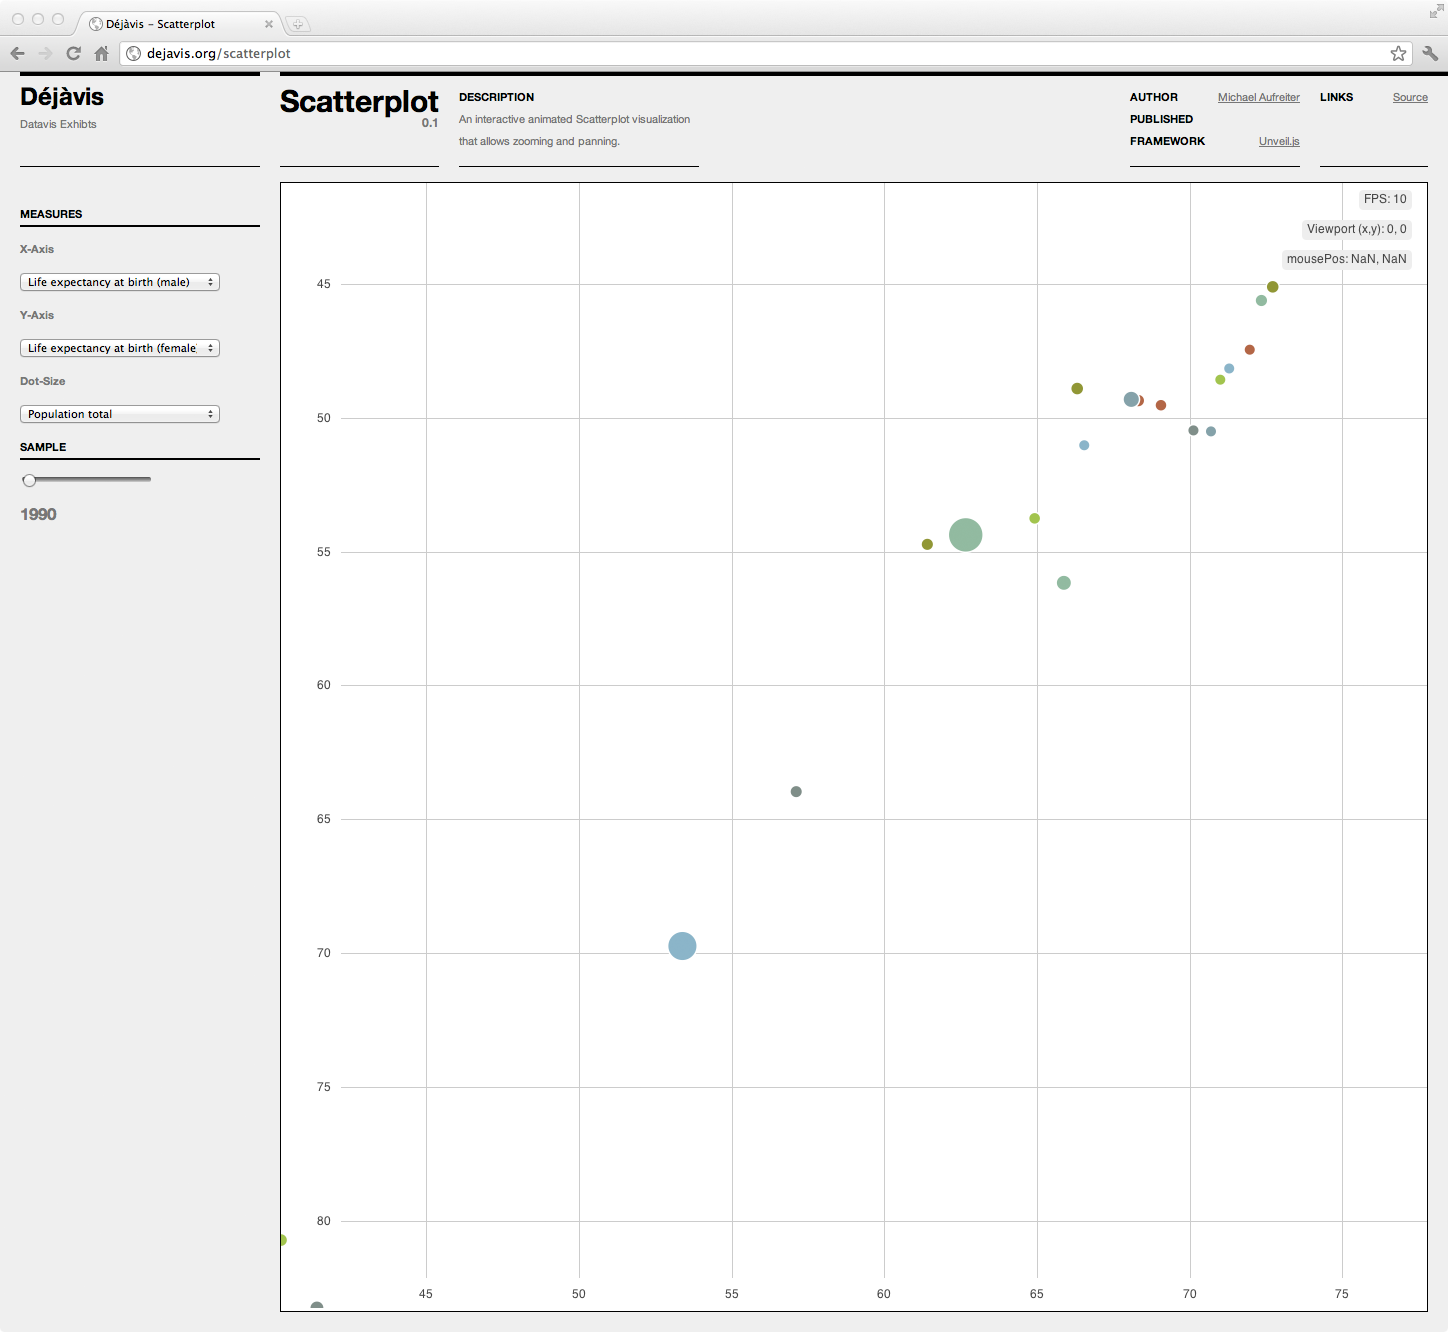
\includegraphics[width=1\textwidth]{scatterplot}
\caption{Scatterplot: A zoomable scatterplot visualization showing indicators for countries in three dimensions encoded using x-Axis, y-Axis and dot size.}
\label{fig:scatterplot}
\end{figure}

Scatterplot\footnote{http://github.com/michael/scatterplot}, as shown in Figure \ref{fig:scatterplot}, is an implementation of a zoomable scatterplot visualization that takes data in a uniform \texttt{Data.Collection} format. Users can assign different properties to certain axes. Each time they are changed, an animated transition takes place. Scatterplot makes intensive use of the data manipulation utilities provided by Data.js as well as matrix transformations for implementing zoom and pan behavior.


\subsection{Stacks}
%%%-----------------------------------------------------------------------------

Stacks\footnote{http://github.com/michael/stacks}, as shown in Figure \ref{fig:stacks}, is a visualization of categorical data. Musical Artists are displayed using self-organizing stacks that hold items of a certain group (e.g. genres like pop music, jazz, etc.). Based on meta-data, users can choose from ordinal properties that should be used to calculate group memberships. Transitions are animated accordingly. 

\begin{figure}
\centering
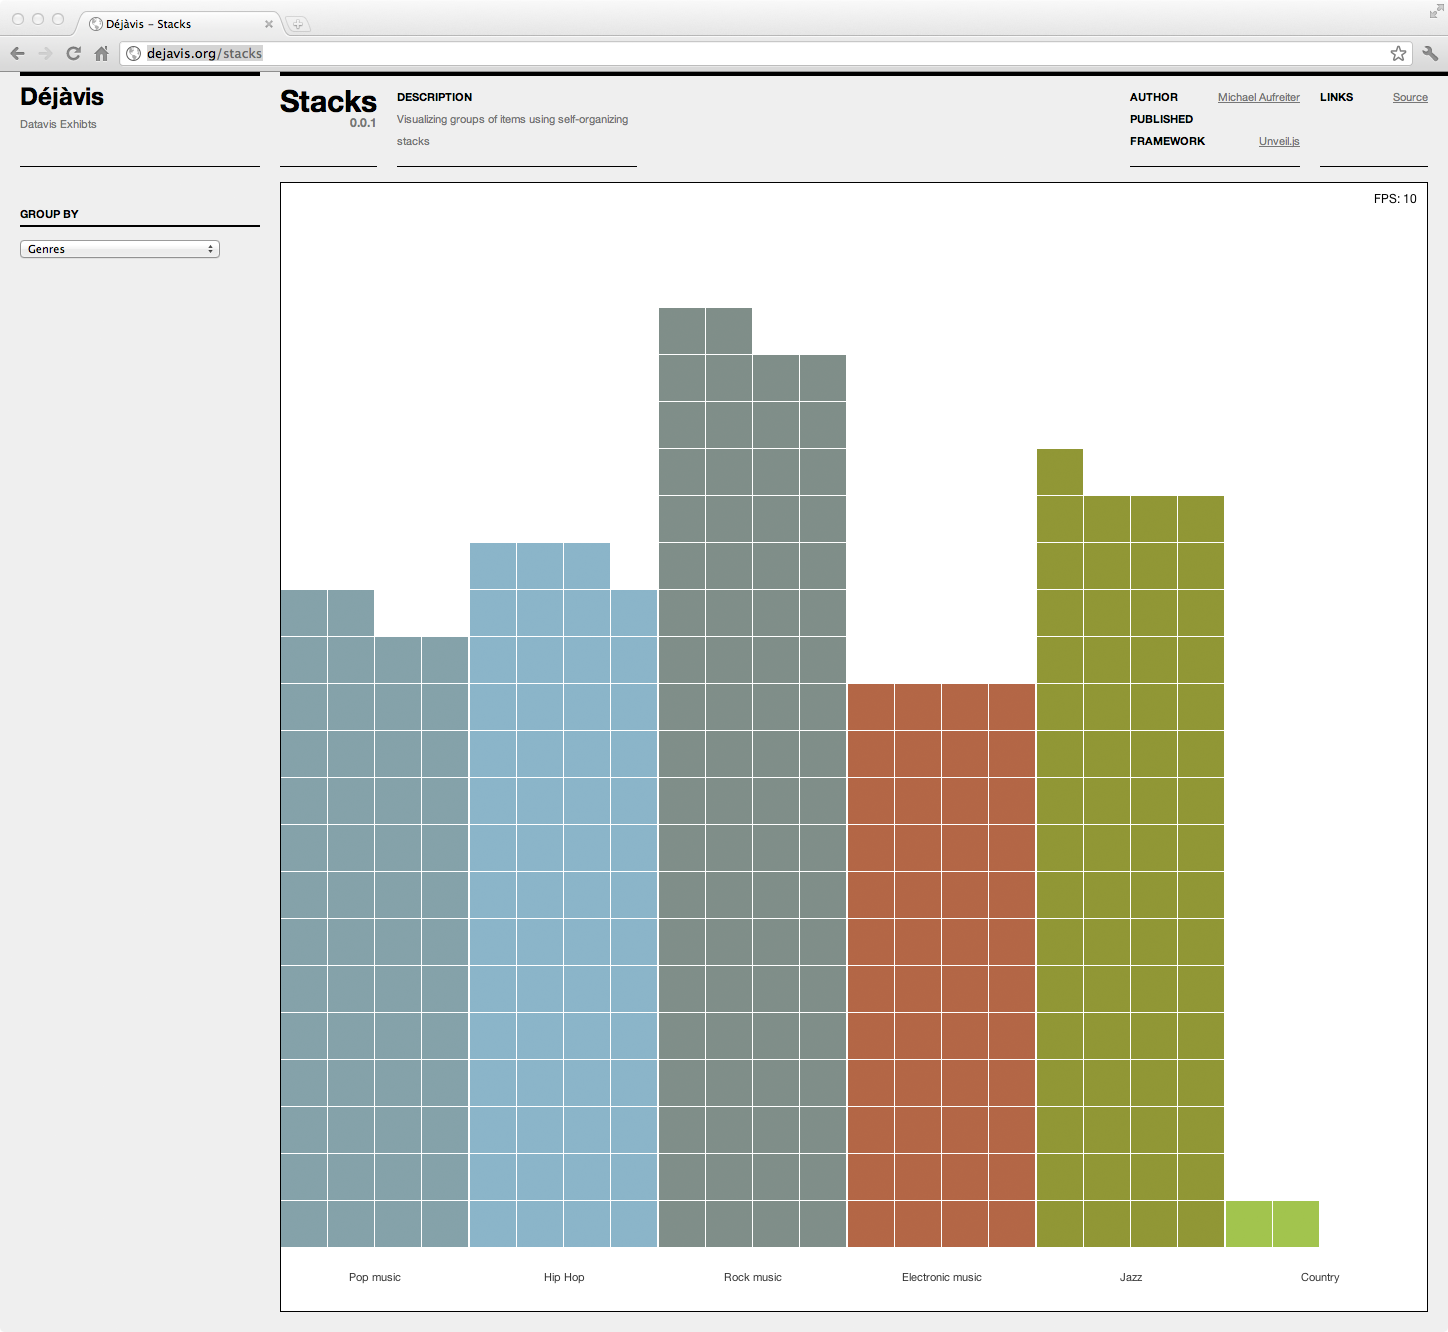
\includegraphics[width=1\textwidth]{stacks}
\caption{Self-organizing Stacks: Based on a layout algorithm groups and items are arranged on the screen.}
\label{fig:stacks}
\end{figure}

\end{english}
\chapter{Evaluation}
\label{cha:evaluation}

In this chapter, the quality of two selected toolkits is examined based on the requirements that were defined in Chapter~\ref{cha:requirements}. The basic goal is to show strengths and weaknesses of existing solutions with the aim to to give visualization authors the chance to pick the right tool for a certain task. This evaluation is used to examine the quality of Unveil.js, the author's contribution to the set of available visualization toolkits. The result should give information about whether the design goals have been met or not. D3.js has been selected for comparison, since it uses a fundamentally different strategy for solving the same sort of problems (animation, interaction). The comparison of these two frameworks drives a discussion about strengths and weaknesses of each approach. Additionally, a benchmark has been implemented for the comparison of rendering performance.

\section{Methodology}
%%%-----------------------------------------------------------------------------

Because of the versatile characteristics of programming languages, visualizations toolkits and visualizations in general the following discourse does not claim to be an exact evaluation of quantitative measures telling the true quality of certain solutions. There is no meaningful approach to determine the exact value of examined toolkits based on quantitative measures. In our evaluation, toolkits receive scores for each requirement. 

% In order to allow a refined total score we use different weights (Figure~\ref{tab:weighting}) for the requirements, as their individual importance for the overall qualification differs.

% \subsection{Scoring System}
%%%-----------------------------------------------------------------------------

The possible scores (Figure~\ref{tab:scoring}) per requirement range from 0 (not supported or insufficient quality) to 3 (complete support or very high quality).

\begin{table}
\caption{Scoring System}
\label{tab:scoring}
\centering
\setlength{\tabcolsep}{5mm} % separator between columns
\def\arraystretch{1.25} % vertical stretch factor
\begin{tabular}{|r||c|c|c|} \hline
Score & \emph{Level of Support} & \emph{Quality}\\
\hline\hline
3 & complete & very high \\
\hline
2 & good & satisfying \\
\hline
1 & basic & sufficient \\
\hline
0 & not supported & insufficient \\
\hline
\end{tabular}
\end{table}


% \subsection{Weighting}
% %%%-----------------------------------------------------------------------------
% 
% Based on the explanations by Bostock and Heer~\cite{D3}, we use a higher weight for \textit{Declarative Language Design} and a lower weight for \textit{Cross-platform Deployment}, since our evaluation is dedicated to web-based deployment. In practice, when applying this evaluation framework, weights should be chosen with respect to the concrete evaluation task.


% \begin{table}
% \caption{Weighting of evaluation requirements}
% \label{tab:weighting}
% \centering
% \setlength{\tabcolsep}{5mm} % separator between columns
% \def\arraystretch{1.25} % vertical stretch factor
% \begin{tabular}{|r||c|c|c|} \hline
% \emph{Criterion}                         & \emph{Weight} \\
% \hline\hline
% Declarative Language Design              & 17\% \\
% \hline
% Cross-platform Deployment                & 5\% \\
% \hline
% Optimization                             & 13\% \\
% \hline
% Data Representation and Transformation   & 13\% \\
% \hline
% Object-oriented Composition              & 13\% \\
% \hline
% Interaction                              & 13\% \\
% \hline
% Animation                                & 13\% \\
% \hline
% Extensibility                            & 13\% \\
% \hline
% \end{tabular}
% \end{table}


\section{Unveil.js}
%%%-----------------------------------------------------------------------------

Unveil.js, as described in Chapter~\ref{cha:unveil}, is a data-driven visualization toolkit, providing a slim abstraction in the form of a Scene API on top of the HTML5 Canvas element.

\subsection{Declarative Language Design}
%%%-----------------------------------------------------------------------------

Unveil.js uses a declarative scene definition format based on JSON. Users can specify graphical objects, so called Actors, that appear in the scene as well as behavior like interaction with objects. Moreover, animated transitions can be specified by using a simple declarative API.

\SuperPar \textbf{Score: 3}

\subsection{Cross-platform Deployment}
%%%-----------------------------------------------------------------------------

Unveil.js uses a toolkit-specific specification syntax for describing visualizations. By separating specification from execution, it is suitable for retargeting to other platforms. However, Unveil.js is an embedded DSL hosted by the Javascript programming language. This implies that porting it to other platforms is constrained to the Javascript scripting environment. Given that Javascript is available outside of the browser (Rhino\footnote{http://www.mozilla.org/rhino}, Node.js\footnote{http://nodejs.org}) visualizations can be retargeted to run in these environments.


\SuperPar \textbf{Score: 1}


\subsection{Optimization}
%%%-----------------------------------------------------------------------------

Since visualization specification is decoupled from implementation, optimizations can be applied by the language designer~\cite{DeclarativeLD10}. There are many options for optimization, such as improving the evaluation and rendering stages. With some effort, supporting new rendering platforms (such as WebGL) is also possible without changing the scene definition language.

\SuperPar \textbf{Score: 3}

\subsection{Data Representation and Transformation}
%%%-----------------------------------------------------------------------------

Unveil.js comes with extended support for data representation and transformation. Through Data.js it supports data abstraction formats for both tabular data (\texttt{Data.Collection}) and linked data (\texttt{Data.Graph}). Unveil.js promotes the creation of highly data-driven visualizations, which can not only use raw data but also meta-data, giving information about how a particular dataset is structured.

\SuperPar \textbf{Score: 3}

\subsection{Object-oriented Composition}
%%%-----------------------------------------------------------------------------

Unveil.js features some pre-implemented graphical objects (Actors). The object-oriented design should encourage users to think in graphical objects, which makes the process of creating complex visualizations easier. New customized Actors can be derived from existing actors or aggregate lower level actors to higher level ones that form reusable modules. In Unveil.js, the creation of new actors is a fundamental part of the visualization creation process.

\SuperPar \textbf{Score: 3}

\subsection{Interaction}
%%%-----------------------------------------------------------------------------

Unveil.js provides support for event handlers that can be bound to graphical objects. With the regular Canvas API this would not be possible because graphical objects are not tracked. In order enable interaction, hit testing, based on \texttt{isPointiInPath}, must be implemented for each Actor. In terms of performance, Unveil.js detects if interaction could potentially happen (e.g. when the mouse cursor is moved) and allocates resources (in the form of an increased frame rate) only on demand. For custom objects, however, users need to specify a corresponding bounding box themselves, which can be difficult and time-consuming for complex forms.

\SuperPar \textbf{Score: 2}

\subsection{Animation}
%%%-----------------------------------------------------------------------------

Unveil.js adds support for animation of graphical properties through the \texttt{animate} method provided by Actors. 

As it is the case with interaction, the frame rate of the visualization becomes increased only demand to keep overall CPU utilization low. Since the HTML5 Canvas element is used for rendering, Unveil.js is suitable for simultaneously animating large numbers of objects.

\SuperPar \textbf{Score: 3}

\subsection{Extensibility}
%%%-----------------------------------------------------------------------------

Extensibility is realized through the Actor abstraction, that enables users to compose higher level objects. These objects are derived from or composed of lower level graphical primitives. Actors can be used not only for graphical primitives but also for abstracting real world objects (carrying data and state) and encapsulating interaction and animation.

\SuperPar \textbf{Score: 3}


\section{D3.js}
%%%-----------------------------------------------------------------------------

D3.js is similar to its predecessor Protovis and offers comparable notational efficiency but differs in the method of implementation as the native representation (DOM) is directly exposed by the interface.

\subsection{Declarative Language Design}
%%%-----------------------------------------------------------------------------

D3 provides a declarative interface for specifying document transformations based on data. While Protovis focussed on the specification of static scenes, D3 offers an interface for specifying dynamic visualizations involving animation and interaction. In order to utilize the notational efficiency of specialized graphical primitives that are not offered by SVG directly, the \texttt{d3.svg} module provides various shapes suitable for charting. 

\SuperPar \textbf{Score: 3}

\subsection{Cross-platform Deployment}
%%%-----------------------------------------------------------------------------

D3 uses a representation transparent approach and relies on the document object model, and thus on web-native technologies (HTML, SVG and CSS). Consequently, this implies that visualizations specified using D3~\cite{D3} cannot be deployed to platforms other than the web. This is by design, according to Michael Bostock, and in turn offers better accessibility, while transformations of the DOM offer dramatic performance gains.

\SuperPar \textbf{Score: 0}

\subsection{Optimization}
%%%-----------------------------------------------------------------------------

The result of D3 document transformations is a scene graph, represented as DOM elements. Overall visualization performance depends on the performance offered by browsers. There is no intermediate representation (such as a toolkit-specific scene graph) that could be optimized in terms of evaluation or rendering. This is all up to the native browser technologies, such as Javascript, SVG and CSS. Because the DOM is modified directly, D3 can avoid unnecessary computation, as transformations can be limited to selected attributes. The author assigns a score of 2 here, as D3.js performance can be considered good. However, the design of this library intentionally does not offer much room for rendering optimization.

\SuperPar \textbf{Score: 2}

\subsection{Data Representation and Transformation}
%%%-----------------------------------------------------------------------------

D3 works with Javascript-native data structures, such as arrays and objects. There are a number of utility functions available, e.g. for working with dates, scales and colors. D3, however, lacks support for higher level data-abstraction. Since Data.js is available as a separate library, D3 users could use it to fill this gap.

\SuperPar \textbf{Score: 1}

\subsection{Object-oriented Composition}
%%%-----------------------------------------------------------------------------

As a consequence of not introducing a scene graph abstraction, D3.js lacks an object oriented interface. An object-oriented programming model often helps with thinking and abstracting from real world objects. D3.js gives users full freedom about how they can structure their code and fits well into the Javascript programming model. However, depending on the programming background of the user it might complicate learning the language and dealing with complex visualization tasks.

\SuperPar \textbf{Score: 0}


\subsection{Interaction}
%%%-----------------------------------------------------------------------------

With D3, adding interaction is easy. Because the DOM is exposed, event handlers can be attached to graphical objects directly. Programmers, who have done web-development or have used DOM manipulation libraries such as jQuery\footnote{http://jquery.com/} will immediately be familiar with it. D3 also makes data objects available to event handlers, allowing data-driven interaction.

\SuperPar \textbf{Score: 3}

\subsection{Animation}
%%%-----------------------------------------------------------------------------

Being the official successor of Protovis, D3.js comes with comprehensive support for transitions, where attributes or styles are smoothly interpolated over time. Animated transitions can be specified using the transition operator. There is support for staggered animation through individual specification of delay and duration. The easing method can be customized too. Performance experiments have shown that animation works well with a moderate number of motion tweens running at the same time. If the number of animated objects become too high, rendering performance drops significantly. In such scenarios, the Canvas Rendering API has some advantages.

\SuperPar \textbf{Score: 3}

\subsection{Extensibility}
%%%-----------------------------------------------------------------------------

D3 can be extended through optional modules which can be included as needed without bloating the library's core. There are numerous modules available, such as the \texttt{geo} module, which adds support for geographic data or the \texttt{geom} module, which adds computational geometry utilities (e.g. layout algorithms). Moreover, the layout module is an important one, as it is providing various reusable visualization layouts, such as force-directed graphs, treemaps and chord diagrams. The module system can be used by D3.js users to build extensions that can easily be adapted by others.

\SuperPar \textbf{Score: 3}


\section{Performance Evaluation}

\begin{figure}
\centering
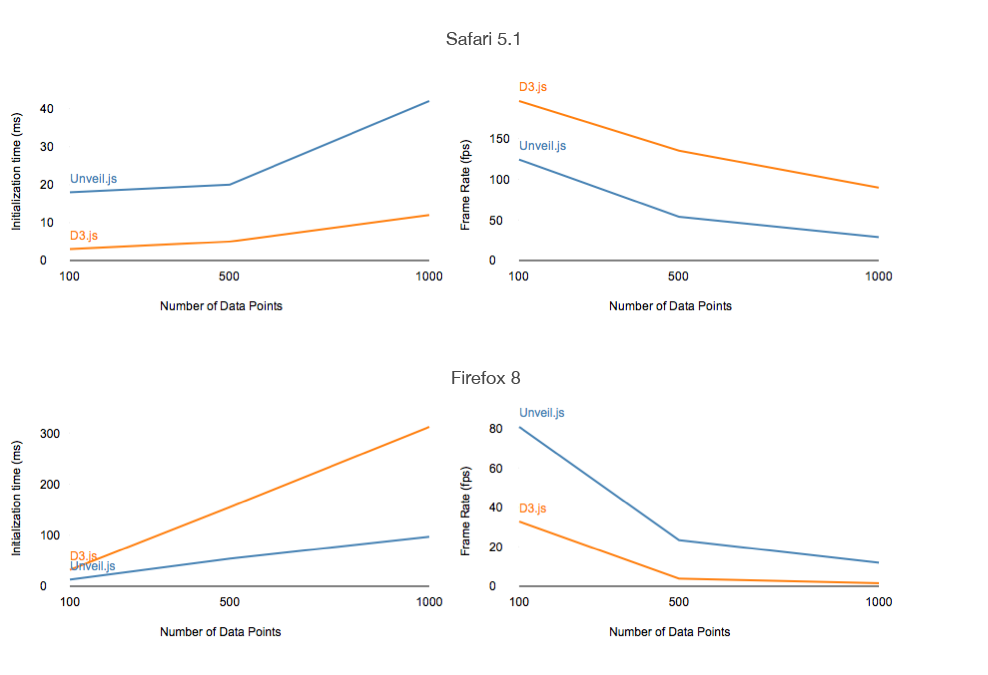
\includegraphics[width=1\textwidth]{benchmarks}
\caption{Performance benchmarks. Initialization times (left) and frames rates (right) for Safari (top) and Firefox (bottom).}
\label{fig:benchmarks}
\end{figure}

In addition to the qualitative evaluation based on requirements, a performance benchmark has been implemented that opposes Unveil.js with D3.js. 
The benchmark considers initialization times and frame rates by constructing a scatterplot using different numbers of objects. The results, as shown in Figure~\ref{fig:benchmarks}, reveal that overall performance highly depends on the browser's implementation of native interfaces (HTML Canvas and SVG). Current webkit-based browsers (Google Chrome, Safari) provide high performance rendering for the SVG interface, which makes D3 noticeably faster here. Moreover profiling results have shown that Unveil.js performance (compared to native usage of the Canvas element) is decreased due to the application of matrix transformations. Unveil.js uses its own matrix library in order to let users adjust the object drawing order. However, this has been identified as a significant bottleneck and should be optimized in future.

In general both libraries offer sufficiently fast performance to implement interactive visualizations involving animation. Importantly, the results shown in the benchmark are just a snapshot considering a single use-case. According to the explanations in the qualitative evaluation, visualization designers need to decide themselves, which is the best solution for a particular task.

\section{Summary}

\begin{table}
\caption{Comparison of individual scores between Unveil.js and D3.js}
\label{tab:comparison}
\centering
\setlength{\tabcolsep}{5mm} % separator between columns
\def\arraystretch{1.0} % vertical stretch factor
\begin{tabular}{|r||c|c|c|} \hline
\emph{Requirement} & \emph{Unveil.js} & \emph{D3.js}\\
\hline\hline
Declarative Language Design & 3 & 3\\
\hline
Cross-platform Deployment & 1 & 0\\
\hline
Optimization & 3 & 2\\
\hline
Data Representation and Transformation & 3 & 1 \\
\hline
Object-oriented Composition & 3 & 0 \\
\hline
Interaction & 2 & 3 \\
\hline
Animation & 3 & 3 \\
\hline
Extensibility & 3 & 3 \\
\hline
% Total Score &  & 2.77 & 2.07 \\
% \hline
\end{tabular}
\end{table}

The toolkits examined both try to solve the same range of issues involving \emph{expressive methods of specification} and solutions for \emph{animation} and \emph{interaction}. D3.js, on the one hand, uses a representation transparent approach and intentionally abandons the possibility of cross-platform deployment. Instead, it focuses on providing a simplified interface to interact with web-native technology. Unveil.js, in turn, targets highly data-driven visualization tasks using a toolkit specific abstraction for describing scenes. It has its focus on modularization and code-reuse and uses an object-oriented approach to match the mental model of real world objects. 



% The scores do not reflect the overall quality of evaluated toolkits, they just emphasize the support of different requirements.

While D3's expressive syntax and deep integration with developer tools is suitable for many visualization tasks, Unveil.js may be a good fit when it comes to approaching complex visualization tasks through object-oriented abstraction.

In addition, Unveil.js contributes Data.js, a comprehensive data manipulation framework that offers a programmatic interface to domain data.
\chapter{Conclusion and Outlook}
\label{cha:conclusion}

% \section{Results}

In the course of this MSc Thesis, a functioning visualization toolkit has been developed. Unveil.js uses a toolkit-specific abstraction for visualization specification. The evaluation has shown that the results are sufficiently fast. Unveil.js has strengths in object-oriented composition, but weaknesses in supporting interaction due to the characteristics of the HTML5 Canvas element. Moreover, it contributes Data.js, a comprehensive data-manipulation component that can also be utilized in other frameworks (e.g. D3.js).

% \section{Caveats}
%  ---------------------------------------------------

Declarative interfaces have been considered a suitable way to approach visualization development in web-based environments~\cite{Protovis09}. Because of the dynamic nature of Javascript and native support for JSON as an established data exchange format, toolkits that favor a declarative interface have been found advantageous over classical imperative programming models.

Within the context of declarative tools, there is a discussion about whether to choose a representation-transparent approach~\cite{D3} or to use a toolkit-specific specification syntax. While an representation-transparent approach improves expressiveness and simplifies debugging, toolkit-specific abstractions are often easier to understand, allow cross-platform deployment and can be optimized independently (because execution is separated from specification). The decision which approach is appropriate for a certain use-case, however, is left to the developer.

Simple visualization tasks can often be accomplished by employing the DOM interface directly. However, for more complex scenarios, employing a toolkit (e.g. Unveil.js or D3.js) could make sense, especially if interaction is needed. If interaction is not a requirement, using the raw Canvas API seems reasonable.

Finally, visualization designers have to decide whether or not to use web-based technology for their particular visualization task. Generally spoken, web-based visualization should be considered if the results are intended for a broader audience. If capabilities are sufficient in terms of data-throughput, rendering performance needs to be evaluated for a particular task. For ad-hoc visualizations which need not to be shared publicly or involve huge amounts of data, using native desktop technology is probably a better choice. An example for this would be medical visualization such as plotting a CT. Given an abstract visualization specification and support for both web and desktop runtime environments, cross-platform deployment would be possible. Unfortunately, in practice production-ready frameworks suitable for cross-platform deployment are not yet available.

\SuperPar Within the last years, web-native technologies have made good progress. Javascript implementations become measurably faster every month. Javascript emerges as a platform and is no longer restricted to the browser environment. Server side implementations, such as Rhino\footnote{http://www.mozilla.org/rhino} or the ambitious Node.js\footnote{http://nodejs.org}, are ready for production use.

Considering that browsers have already started to gain hardware acceleration support for graphical operations, it is likely that in the near future web-native technologies with respect to Information Visualization will be on par with traditional graphics programming environments.

However, even if low level interfaces are continuously improved, there is a great demand for higher level interfaces. Tools that have been covered in this thesis are just a start. API's should influence each other in order to create better abstractions. Moreover, the availability of expressive abstractions may influence browser-native API's as well. A prominent example for this is the upcoming ECMAScript 6 Standard. It will contain language constructs adapted from CoffeeScript\footnote{http://coffeescript.org}, a higher-level language that compiles to Javascript and exposes a simpler syntax. In the same way high quality visualization toolkits could influence native graphical interfaces. Every developer is enabled to contribute here, as it is not just up to the specification committee (W3C\footnote{http://www.w3.org/}) how future graphical interfaces will look like.


%%%----------------------------------------------------------
%%%Anhang

\appendix



%%%----------------------------------------------------------

%Literaturverzeichnis
\clearpage 
\addcontentsline{toc}{chapter}{\bibname}
\bibliographystyle{bababbrv} 
%options: babplain, babunsrt, bababbrv, babalpha 
%         babplain-fl etc: first/lastname 
%         babplain-lf etc: last/firstname
\bibliography{literatur}     %BibTeX-Datei literatur.bib


%%%----------------------------------------------------------

%%%Messbox zur Druckkontrolle
% \chapter*{Messbox zur Druckkontrolle}



\begin{center}
{\Large --- Druckgr��e kontrollieren! ---}

\bigskip

\Messbox{100}{50} % Angabe der Breite/Hoehe in mm

\bigskip

{\Large --- Diese Seite nach dem Druck entfernen! ---}

\end{center}



\end{document}
